De nombreux phénomènes dépendent de plusieurs paramètres, par exemple le volume d'un gaz dépend de la température et de la pression; l'altitude $z$ d'un terrain dépend des coordonnées $(x,y)$ du lieu.

Dans les réseaux de neurones, les fonctions de plusieurs variables interviennent de deux manières :
\begin{itemize}
	\item lors de l'utilisation d'un réseau. C'est la partie la plus facile et la plus fréquente. On utilise un réseau déjà bien paramétré pour répondre à une question (Est-ce une photo de chat ? Tourner à droite ou à gauche ? Quel pion déplacer au prochain coup ?). La réponse est un calcul direct obtenu en évaluant une fonction de plusieurs variables. 
	
	\item lors de la paramétrisation du réseau. C'est la partie difficile et le but de ce cours. Quels paramètres choisir pour définir ce réseau afin qu'il réponde au problème ? Ces paramètres seront choisis comme minimum d'une fonction de plusieurs variables. Une des difficultés est qu'il peut y avoir des milliers de paramètres à gérer.
	
\end{itemize}



%%%%%%%%%%%%%%%%%%%%%%%%%%%%%%%%%%%%%%%%%%%%%%%%%%%%%%%%%%%%%%%%%%%%%
\section{Définition et exemples}

%--------------------------------------------------------------------
\subsection{Définition}


Nous allons étudier les fonctions de deux variables, mais aussi de trois variables et plus généralement de $n$ variables.
Ces fonctions sont donc de la forme 
$$f : \Rr^n \rightarrow \Rr$$
où $n$ est un entier naturel supérieur ou égal à $1$. 


Un élément de l'ensemble de départ est un vecteur de type  $x = (x_1,\ldots,x_n)$. À chacun de ces vecteurs, $f$ associe un nombre réel $f(x_1,\ldots,x_n)$. On pourrait aussi limiter l'ensemble de départ à une partie $E$ de $ \Rr^n$.



%--------------------------------------------------------------------
\subsection{Deux variables}

Lorsque $n=2$, on préfère noter les variables $(x,y)$ plutôt que $(x_1,x_2)$.
Voici quelques exemples.
\begin{exemple}{}{}
	
	\begin{itemize}
		\item $f(x,y) = 2x+3y^2+1$.
		\item $f(x,y) = \cos(xy)$.
		\item $f(x,y) = \sqrt{x^2+y^2}$. $f$ renvoie la distance entre un point $M(x,y)$ et l'origine $O(0,0)$.
		
		\myfigure{1}{
			\tikzinput{fig-fonctions-01}
		}
		
		\item L'équation physique $PV=nRT$ implique $T = \frac{1}{nR}PV$ :
		la température d'un gaz s'exprime en fonction de son volume et de la pression ($n$ et $R$ sont des constantes).
		\item La distance entre une droite fixée $\mathcal{D}$ d'équation $ax+by+c=0$ et un point $M(x_0,y_0)$ est donnée par une fonction de deux variables : $$d(x_0,y_0) = d(M,\mathcal{D}) = \frac{|ax_0+by_0+c|}{\sqrt{a^2+b^2}}.$$
		
		\myfigure{1}{
			\tikzinput{fig-fonctions-02}
		}
		
		
	\end{itemize}
\end{exemple}


%--------------------------------------------------------------------
\subsection{Trois variables}

\begin{exemple}{}{}
	
	\begin{enumerate}
		\item $f(x,y,z) = ax+by+cz+d$. Cette fonction $f$ est une fonction affine ($a,b,c,d$ sont des constantes).
		\item $f(x,y,z) = x^2+y^2+z^2$ qui donne la distance au carré entre un point $M(x,y,z)$ et l'origine $O(0,0,0)$.
		\item Le volume d'un cône à base rectangulaire dépend des longueurs des côtés $a$ et $b$ de la base et de la hauteur $h$ :
		$$V = f(a,b,h) = \frac13 abh.$$
		
		\myfigure{0.5}{
			\tikzinput{fig-fonctions-03}
		}
		
	\end{enumerate}
\end{exemple}


%--------------------------------------------------------------------
\subsection{$n$ variables}

\begin{exemple}{}{}
	
	\begin{enumerate}
		\item $f(x_1,\ldots,x_n) = a_1x_1+\cdots+a_nx_n+a_0$ une fonction affine (les $a_i$ sont des constantes).
		\item $f(x_1,\ldots,x_n) = \sqrt{(x_1-a_1)^2+\cdots+(x_n-a_n)^2}$ exprime la distance entre les points $M(x_1,\ldots,x_n)$ et $A(a_1,\ldots,a_n)$ dans $\Rr^n$.
	\end{enumerate}
\end{exemple}


%%%%%%%%%%%%%%%%%%%%%%%%%%%%%%%%%%%%%%%%%%%%%%%%%%%%%%%%%%%%%%%%%%%%%
\section{Graphe}

Le cas le plus simple, et déjà connu, est celui des fonctions d'une seule variable $f : \Rr \rightarrow \Rr$.  C'est l'ensemble de tous les points du plan de la forme $(x,f(x))$. Voici le graphe de la fonction $x \mapsto x\cos x$.

\myfigure{0.8}{
	\tikzinput{fig-fonctions-04}
} 



%--------------------------------------------------------------------
\subsection{Définition}

\begin{definition}{}{}
	Le \trouer{graphe} $\mathcal{G}_f$ d'une fonction de deux variables $f : \Rr^2 \to \Rr$ est  l'ensemble des points de $\Rr^3$ ayant pour coordonnées $(x,y,f(x,y))$, pour $(x,y)$ parcourant $\Rr^2$. Le graphe est donc :
	$$\mathcal{G}_f= \big\{ (x,y,z) \in \Rr^3 \mid (x,y)\in \Rr^2 \text{ et } z=f(x,y)\big\}.$$
\end{definition}

Dans le cas de deux variables, le graphe d'une fonction est une surface tracée dans l'espace.


\myfigure{0.7}{
	\tikzinput{fig-fonctions-05}
}


\begin{exemple}{}{}
	On souhaite tracer le graphe de la fonction définie par :
	$$f(x,y) = x  e^{-x^2-y^2}.$$
	
	On commence par tracer quelques points à la main :
	\begin{itemize}
		\item si $(x,y) = (0,0)$ alors $f(x,y) = f(0,0) = 0$ donc le point de coordonnées $(0,0,0)$ appartient au graphe.
		\item Comme $f(1,0) = 1/e$ alors le point de coordonnées $(1,0,1/e)$ appartient au graphe.
		\item Pour n'importe quel $y$, on a $f(0,y)=0$ donc la droite de l'espace d'équation ($x=0$ et $z=0$) est incluse dans le graphe.
		\item Notons $r = \sqrt{x^2+y^2}$ la distance entre le point de coordonnées $(x,y)$ et l'origine $(0,0)$ alors on a la formule $f(x,y) = x e^{-r^2}$. Pour un point éloigné de l'origine, $r$ est grand, donc  $e^{-r^2}$ est très petit, et $f(x,y)$ est très proche de $0$.
	\end{itemize}
	
	
	Voici différentes vues de ce graphe.
	
	\begin{center}
		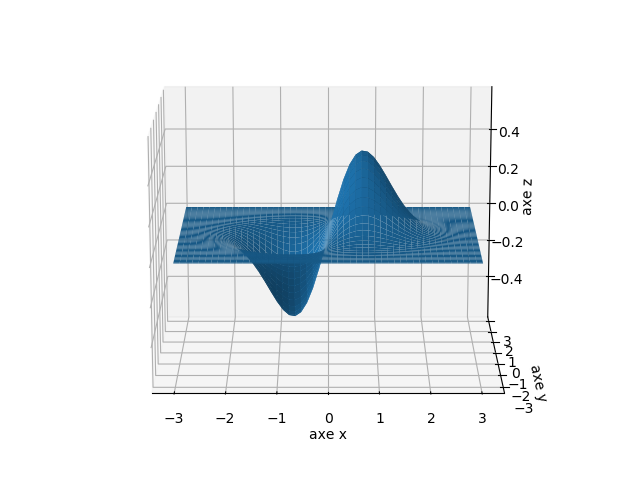
\includegraphics[scale=\myscale,scale=0.5]{figures/fonctions-surface-1a}
		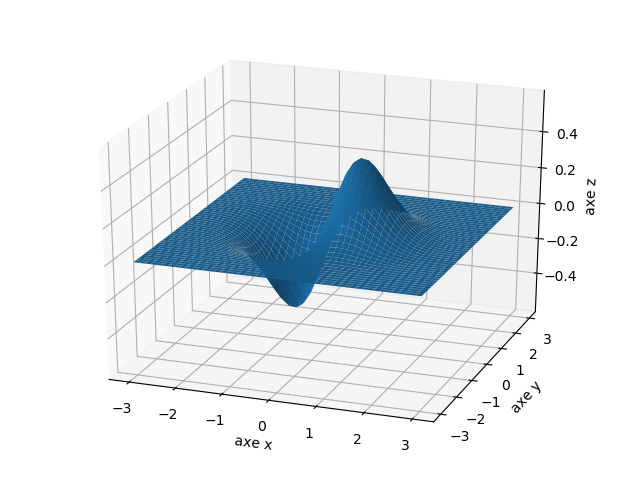
\includegraphics[scale=\myscale,scale=0.5]{figures/fonctions-surface-1b}
		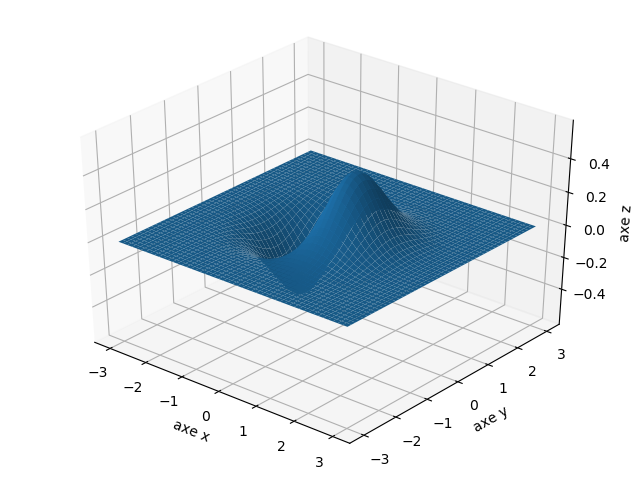
\includegraphics[scale=\myscale,scale=0.5]{figures/fonctions-surface-1c}
		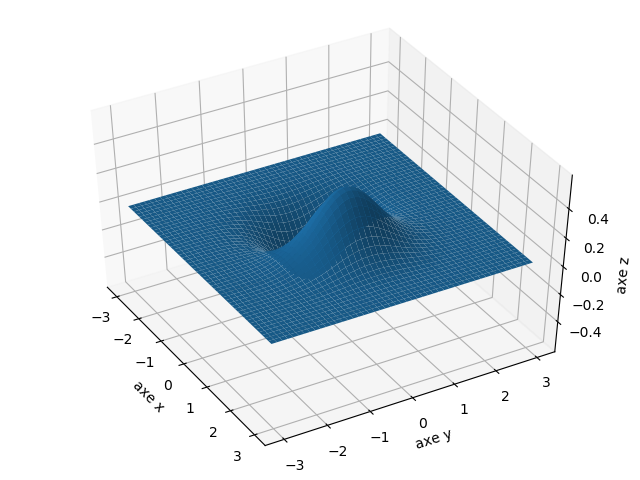
\includegraphics[scale=\myscale,scale=0.5]{figures/fonctions-surface-1d}
	\end{center}
	
	%  fichier python 'fonctions-surface-1.py'
\end{exemple}


%--------------------------------------------------------------------
\subsection{Tranches}

Afin de tracer le graphe d'une fonction de deux variables, on peut découper la surface en \og{}tranches\fg{}.
On fixe par exemple une valeur $y_0$ et on trace dans le plan $(xOz)$ le graphe de la fonction d'une variable  
$$f_{|y_0} : x\mapsto f(x,y_0).$$
Géométriquement, cela revient à tracer l'intersection du graphe de $f$ et du plan d'équation $(y=y_0)$.
On recommence pour plusieurs valeurs de $y_0$, ce qui nous donne des tranches du graphe de $f$ et nous donne une bonne idée du graphe complet de $f$.

On peut faire le même travail en fixant des valeurs $x_0$ avec les fonctions :
$$f_{|x_0} : y \mapsto f(x_0,y).$$


\begin{exemple}{}{}
	On souhaite tracer le graphe de la fonction définie par :
	$$f(x,y) = x \sin(y).$$
	
	\begin{center}
		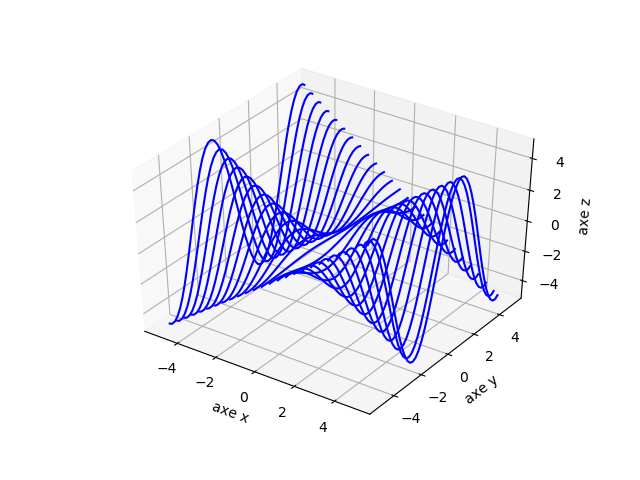
\includegraphics[scale=\myscale,scale=0.5]{figures/fonctions-surface-2a}
		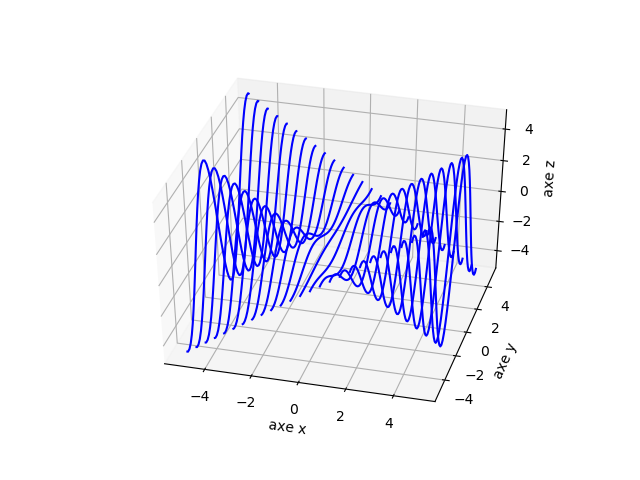
\includegraphics[scale=\myscale,scale=0.5]{figures/fonctions-surface-2b}
		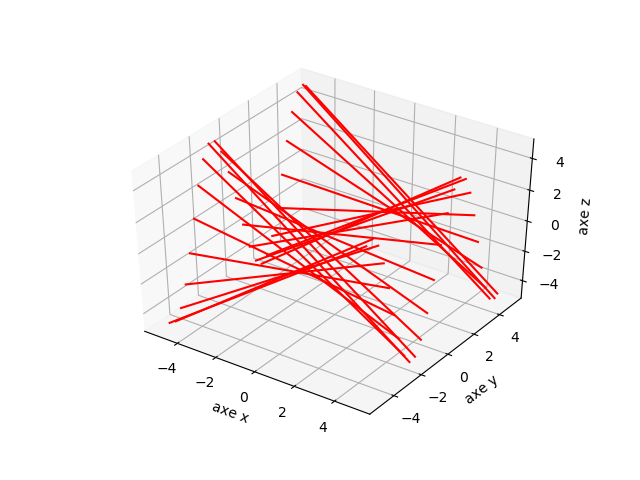
\includegraphics[scale=\myscale,scale=0.5]{figures/fonctions-surface-2c}
		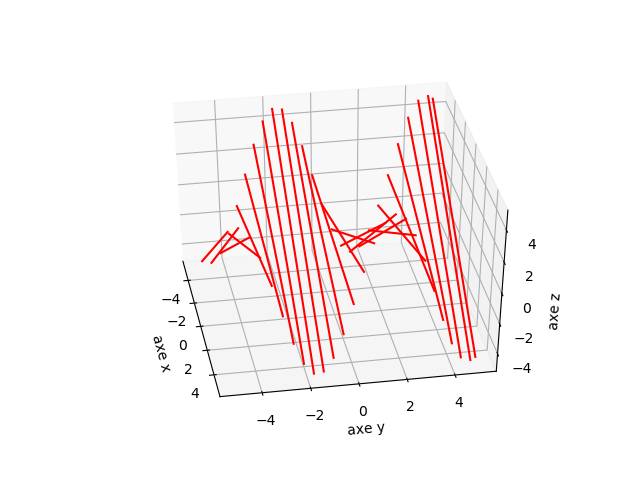
\includegraphics[scale=\myscale,scale=0.5]{figures/fonctions-surface-2d}
		
		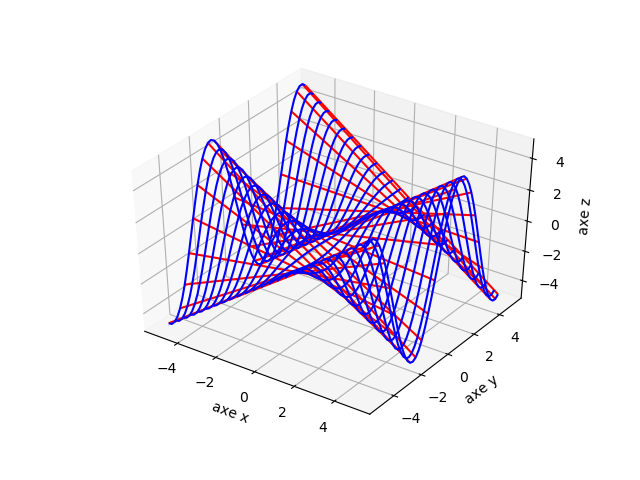
\includegraphics[scale=\myscale,scale=0.7]{figures/fonctions-surface-2e}
	\end{center}
	
	\couleurnb{En bleu}{En haut} les tranches pour lesquelles $x$ est constant (deux points de vue), \couleurnb{en rouge}{au milieu} les tranches pour lesquelles $y$ est constant (deux points de vue). Lorsque l'on rassemble les tranches (à $x$ constant et à $y$ constant), on reconstitue la surface (dernière figure). 
	
	% voir fichier python 'fonctions-surface-2.py'
	
\end{exemple}


%--------------------------------------------------------------------
\subsection{Minimum, maximum}

Pour des fonctions de deux variables (ou plus) il existe une notion de minimum et de maximum.

\begin{definition}{}{}
	\index{minimum!local}
	\index{minimum!global}
	Soit $f : \Rr^2 \to \Rr$ une fonction.
	\begin{itemize}
		\item $f$ atteint un \trouer{minimum global} en $(x_0,y_0) \in \Rr^2$ si
		pour tout $(x,y) \in \Rr^2$, on a $f(x,y) \ge f(x_0,y_0)$.
		
		\item $f$ atteint un \trouer{minimum local} en $(x_0,y_0) \in \Rr^2$ si
		il existe un intervalle ouvert $I$ contenant $x_0$ et un intervalle ouvert $J$ contenant $y_0$  tels que 
		pour tout $(x,y) \in I \times J$, on a $f(x,y) \ge f(x_0,y_0)$. 
	\end{itemize}
\end{definition}



\begin{exemple}{}{}
	Voici l'exemple d'une fonction qui admet deux minimums locaux. L'un est aussi un minimum global. Elle admet un maximum local qui est aussi global.
	
	\begin{center}
		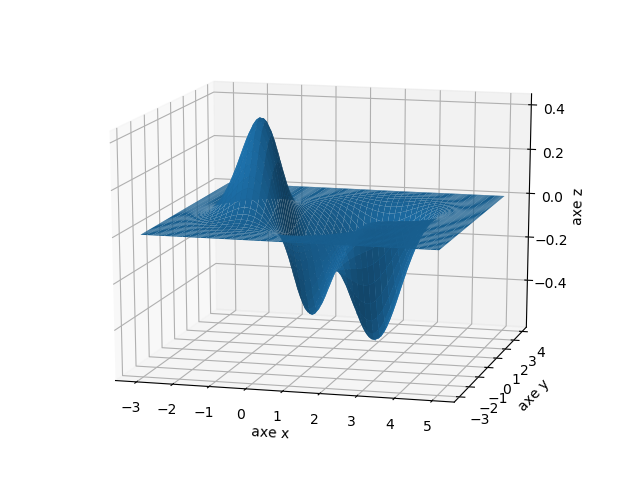
\includegraphics[scale=\myscale,scale=0.7]{figures/fonctions-surface-3}
	\end{center}
	
	% voir fichier python 'fonctions-surface-3.py'
	
\end{exemple}


Trouver les bons paramètres d'un réseau de neurones nous amènera à trouver le minimum d'une fonction de plusieurs (et même de centaines de) variables. Voyons un exemple en deux variables.
\begin{exemple}{}{}
	Étant donnés trois points $A(1,2)$, $B(3,5)$ et $C(6,1)$, il s'agit de trouver un point $M(x,y)$ qui \og{}approche au mieux\fg{} ces trois points. Il faut expliciter une fonction à minimiser pour définir correctement le problème. Nous décidons de prendre la somme des carrés des distances.
	
	
	\myfigure{1}{
		\tikzinput{fig-fonctions-06}
	}
	
	Il s'agit donc de minimiser la fonction $f$ suivante, qui correspond à une fonction distance (aussi appelée fonction erreur ou bien fonction coût) :
	$$f(x,y) = MA^2+MB^2+MC^2 = 
	(x-1)^2+ (y-2)^2 + (x-3)^2 + (y-5)^2 + (x-6)^2 + (y-1)^2.$$
	En développant on trouve :
	$$f(x,y) = 3x^2 + 3y^2 - 20x - 16y + 76.$$
	
	Le graphe de $f$ nous suggère qu'il existe un unique minimum qui est le minimum global de $f$. 
	Par recherche graphique ou par les méthodes décrites dans la section suivante, on trouverait une solution approchée. En fait la solution géométrique exacte est l'isobarycentre des points (autrement dit le centre de gravité du triangle $ABC$), ainsi :
	$$(x_0,y_0) = \left(\frac{10}{3},\frac83\right) \simeq (3.33,2.66)$$
	pour lequel $f$ atteint son minimum $z_0 = f(x_0,y_0) = \frac{64}{3} \simeq 21.33$.
	
	\begin{center}
		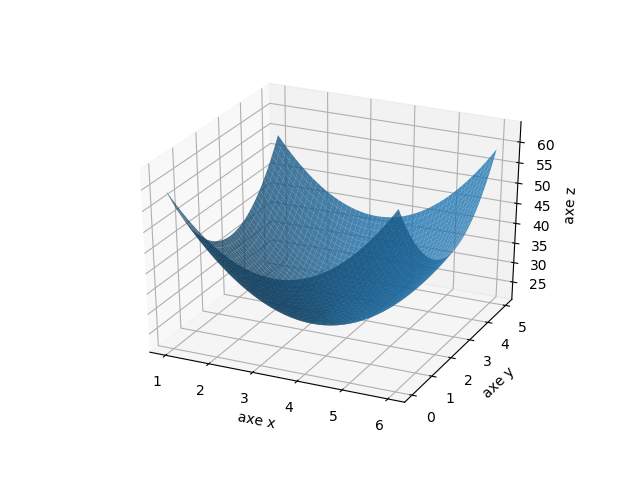
\includegraphics[scale=\myscale,scale=0.7]{figures/fonctions-surface-4}
	\end{center}
	
	% voir fichier python 'fonctions-surface-4.py'
	% voir fichier sage 'fonctions-surface-4.sage' pour résolution exacte
	
	Le point qui convient le mieux à notre problème et en lequel notre fonction distance est minimale est donc le point de coordonnées $(\frac{10}{3},\frac83)$. Attention, un autre choix de la fonction distance $f$ pourrait conduire à une autre solution (voir l'exemple de la prochaine section).
	
	\myfigure{1}{
		\tikzinput{fig-fonctions-07}
	}
	
	
\end{exemple}

%--------------------------------------------------------------------
\subsection{Recherche élémentaire d'un minimum}


Voici trois techniques pour trouver les valeurs approchées des coordonnées du point en lequel une fonction de plusieurs variables atteint son minimum. Ces techniques sont valables quelque soit le nombre de variables même si ici elles ne sont décrites que dans le cas de deux variables. 

\textbf{Recherche sur une grille.} On calcule $f(x,y)$ pour $(x,y)$ parcourant une grille. On retient le point $(x_0,y_0)$ en lequel $z_0=f(x_0,y_0)$ est le plus petit. Si on le souhaite, on peut affiner la grille autour de ce point, en diminuant le pas $\epsilon$ pour améliorer l'approximation. C'est une technique qui demande $N^2$ calculs pour une grille de largeur $N$ (et même $N^n$ pour une fonction de $n$ variables) ce qui peut être énorme.

\myfigure{0.5}{
	\tikzinput{fig-fonctions-08}
}


\textbf{Recherche au hasard.} Cela peut sembler incongru mais choisir quelques coordonnées $(x,y)$ au hasard, calculer chaque valeur $z=f(x,y)$ et comme auparavant retenir le point $(x_0,y_0)$ correspondant au $z_0$ minimal n'est pas ridicule !
Un ordinateur peut tester plusieurs millions de points en quelques secondes. Bien sûr il y a de fortes chances de ne trouver qu'une solution approchée. C'est aussi une technique que l'on retrouvera plus tard : partir d'un point au hasard pour ensuite construire une suite de points convergeant vers un minimum. Et si cela n'est pas concluant, il faudra repartir d'un autre point tiré au hasard.

\bigskip

\textbf{Recherche par tranche.} 
L'idée est de se ramener à des fonctions d'une seule variable. En effet, 
pour les fonctions d'une variable, on sait qu'il faut chercher les minimums là où la dérivée s'annule.

On part d'une valeur $x_0$ (au hasard !). On cherche le minimum sur la tranche $x=x_0$, c'est-à-dire que l'on cherche le minimum de la fonction d'une variable $y \mapsto f(x_0,y)$. On trouve une valeur $y_0$ qui réalise un minimum. On change alors de direction en étudiant maintenant la tranche $y=y_0$ (pour le $y_0$ que l'on vient d'obtenir), on obtient l'abscisse $x_1$ du minimum de la fonction d'une variable $x \mapsto f(x,y_0)$. On recommence depuis le début à partir de ce $x_1$. On obtient ainsi une suite de points $(x_i,y_i)$ avec des valeurs $z_i=f(x_i,y_i)$ de plus en plus petites. On peut espérer tendre vers un minimum. %que $(x_i,y_i)$ tendent vers un minimum.


\myfigure{1}{
	\tikzinput{fig-fonctions-09}
}

Sur la figure ci-dessus, on part d'une tranche \couleurnb{(en bleu) }{}choisie au hasard, donnée par $x=x_0$. Cette tranche définit le graphe d'une fonction d'une variable. On se déplace sur cette courbe jusqu'à atteindre le minimum de cette tranche, en une valeur $y_0$. On considère la tranche perpendiculaire donnée par $y=y_0$. On se déplace sur la courbe \couleurnb{rouge }{}jusqu'à atteindre le minimum de cette tranche, en une valeur $x_1$. On pourrait continuer avec une nouvelle tranche \couleurnb{bleue }{}$x=x_1$, etc.

\bigskip

Les descriptions données ici sont assez informelles, d'une part parce qu'il est difficile d'énoncer des théorèmes qui garantissent d'atteindre un minimum local et d'autre part parce qu'aucune technique ne garantit d'atteindre un minimum global. Lorsque l'on étudiera le gradient, nous obtiendrons une méthode plus efficace.

\begin{exemple}{}{}
	On reprend le problème précédent, à savoir trouver un point $M$ qui approche au mieux les trois points $A$, $B$ et $C$, mais cette fois on choisit la \og{}vraie\fg{} distance comme fonction d'erreur :
	$$g(x,y) = MA+MB+MC = 
	\sqrt{(x-1)^2+ (y-2)^2} + \sqrt{(x-3)^2 + (y-5)^2} + \sqrt{(x-6)^2 + (y-1)^2}.$$
	On applique ces trois techniques pour chercher le minimum de $g$ en se limitant au carré $[0,6]\times[0,6]$.
	
	\begin{enumerate}
		
		\item Avec une grille $N\times N$. Par exemple pour $N=100$, on évalue $g$ en $10\,000$ points. On trouve $(x_{\min},y_{\min}) \simeq (2.91,2.97)$ pour une valeur $z_{\min} \simeq 7.84$. 
		
		\item Avec un tirage aléatoire de $1000$ points, on trouve par exemple :
		$(x_{\min},y_{\min}) \simeq (2.88,2.99)$ et $z_{\min} \simeq 7.84$. Le résultat est similaire à la méthode précédente, bien qu'on ait effectué $10$ fois moins de calculs.
		
		\item Par les tranches. On part de la tranche $(x=0)$. On pose $x_0=0$, la fonction à étudier
		est donc 
		$$g_{|x_0}(y) = \sqrt{1 + (y-2)^2} + \sqrt{9 + (y-5)^2} + \sqrt{36 + (y-1)^2}.$$
		C'est une fonction de la seule variable $y$ pour laquelle on possède des techniques efficaces de recherche de minimum.
		On trouve que le minimum de $g_{|x_0}$ est atteint en $y_0 \simeq 2.45$.
		On recommence avec cette fois la tranche $(y = y_0)$ et on cherche le minimum de la fonction $g_{|y_0}(x) = g(x,y_0)$. On trouve que cette fonction atteint son minimum en $x_1 \simeq 2.84$. 
		On recommence ce processus jusqu'à atteindre la précision souhaitée.
		Ainsi en $5$ étapes on obtient une valeur approchée assez précise du minimum 
		$(x_{\min},y_{\min}) \simeq (2.90579,2.98464)$ et $z_{\min} \simeq 7.83867$.
		
		
	\end{enumerate}
\end{exemple}

La première conclusion à tirer de ce qui précède est que pour résoudre un problème il faut définir correctement une fonction d'erreur, c'est-à-dire celle que l'on cherche à minimiser. La solution trouvée dépend de cette fonction d'erreur choisie. 
Enfin, la méthode des tranches est une méthode efficace pour trouver un minimum d'une fonction, mais nous en découvrirons une encore meilleure en utilisant le gradient.


%%%%%%%%%%%%%%%%%%%%%%%%%%%%%%%%%%%%%%%%%%%%%%%%%%%%%%%%%%%%%%%%%%%%%
\section{Lignes de niveau}

\index{lignes de niveau}

%--------------------------------------------------------------------
\subsection{Définition}

\begin{definition}{}{}
	Soit $f : \Rr^2 \to \Rr$ une fonction de deux variables. 
	La \trouer{ligne de niveau} $z=c\in \Rr$ est l'ensemble de tous les points $(x,y)$ vérifiant $f(x,y)=c$ :
	$$L_c =\big\{(x,y)\in \Rr^2 \mid f(x,y)=c \big\}.$$
\end{definition}

La ligne de niveau $c$ est une courbe du plan $\Rr^2$. 

On peut aussi définir une \trouer{courbe de niveau}, c'est l'ensemble des points de l'espace obtenus comme intersection du graphe $\mathcal{G}_f$ et du plan $z=c$ qui est horizontal et \og{}d'altitude\fg{} $c$. Ce sont donc tous les points $(x,y,f(x,y))$ avec $f(x,y)=c$. On obtient la courbe de niveau en translatant la ligne de niveau d'une altitude $c$.



\begin{exemple}{}{}
	Soit $f : \Rr^2 \to \Rr$ définie par $f(x,y)=x^2+y^2$. 
	
	\begin{itemize}
		\item Si $c<0$, la ligne de niveau $L_c$ est vide (aucun point n'est d'altitude négative).
		\item Si $c=0$, la ligne de niveau $L_0$ se réduit à $\{(0,0)\}$.
		\item Si $c>0$, la ligne de niveau $L_c$  est le cercle du plan de centre $(0,0)$ et de rayon $\sqrt{c}$. On \og{}remonte\fg{} $L_c$ à l'altitude $z=c$ : la courbe de niveau est alors le cercle horizontal de l'espace de centre $(0,0,c)$ et de rayon $\sqrt{c}$. 
	\end{itemize}
	
	Le graphe est alors une superposition de cercles horizontaux de l'espace de centre $(0,0,c)$ et de rayon $\sqrt{c}$, $c>0$.     
	
	Ci-dessous : (a) la surface, (b) $5$ courbes de niveau, (c) $10$ courbes de niveau, (d) les lignes de niveau dans le plan.
	\begin{center}
		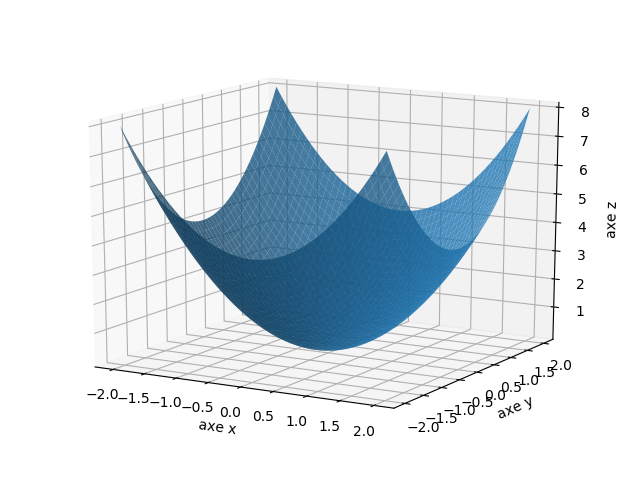
\includegraphics[scale=\myscale,scale=0.5]{figures/fonctions-niveau-1a}
		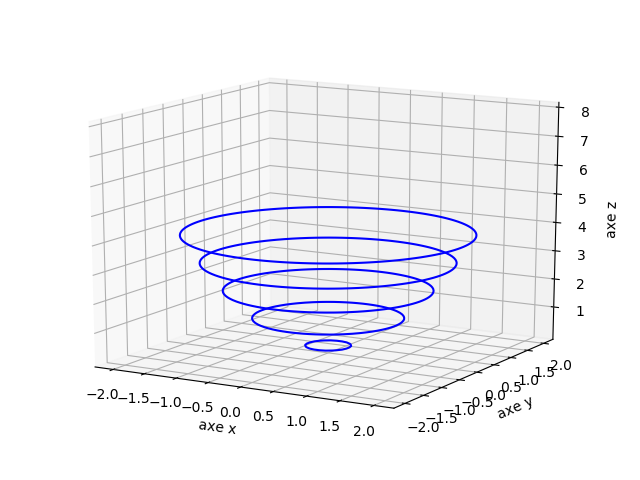
\includegraphics[scale=\myscale,scale=0.5]{figures/fonctions-niveau-1b}
		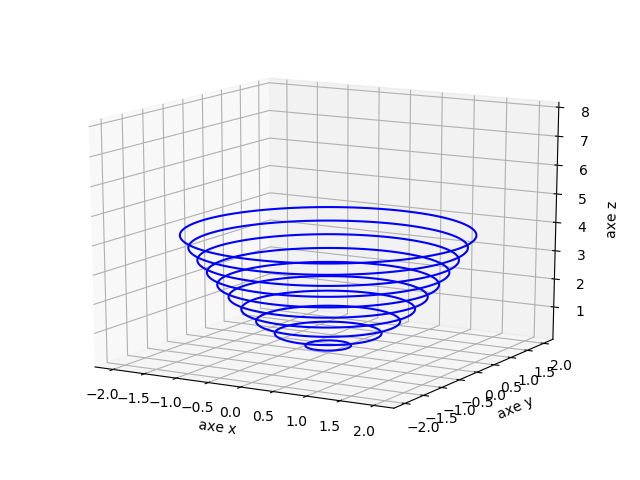
\includegraphics[scale=\myscale,scale=0.5]{figures/fonctions-niveau-1c}
		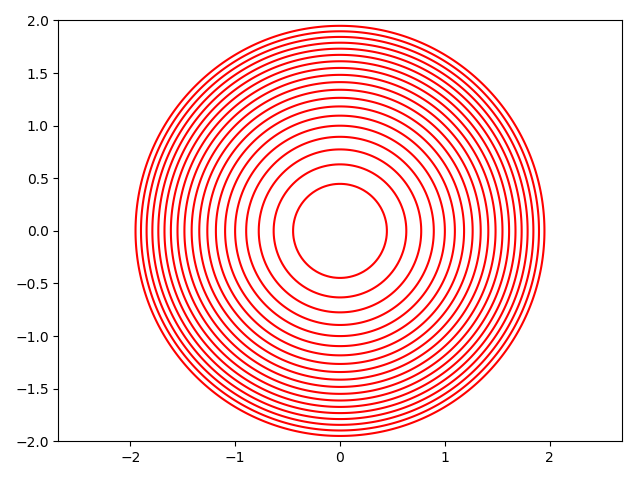
\includegraphics[scale=\myscale,scale=0.5]{figures/fonctions-niveau-1d}
	\end{center}
	
	% dessins 3d voir 'fonctions-niveau-1.py'
	
\end{exemple}


%--------------------------------------------------------------------
\subsection{Exemples}

\begin{exemple}{}{}
	Sur une carte topographique, les lignes de niveau représentent les courbes ayant la même altitude. 
	\begin{center}
		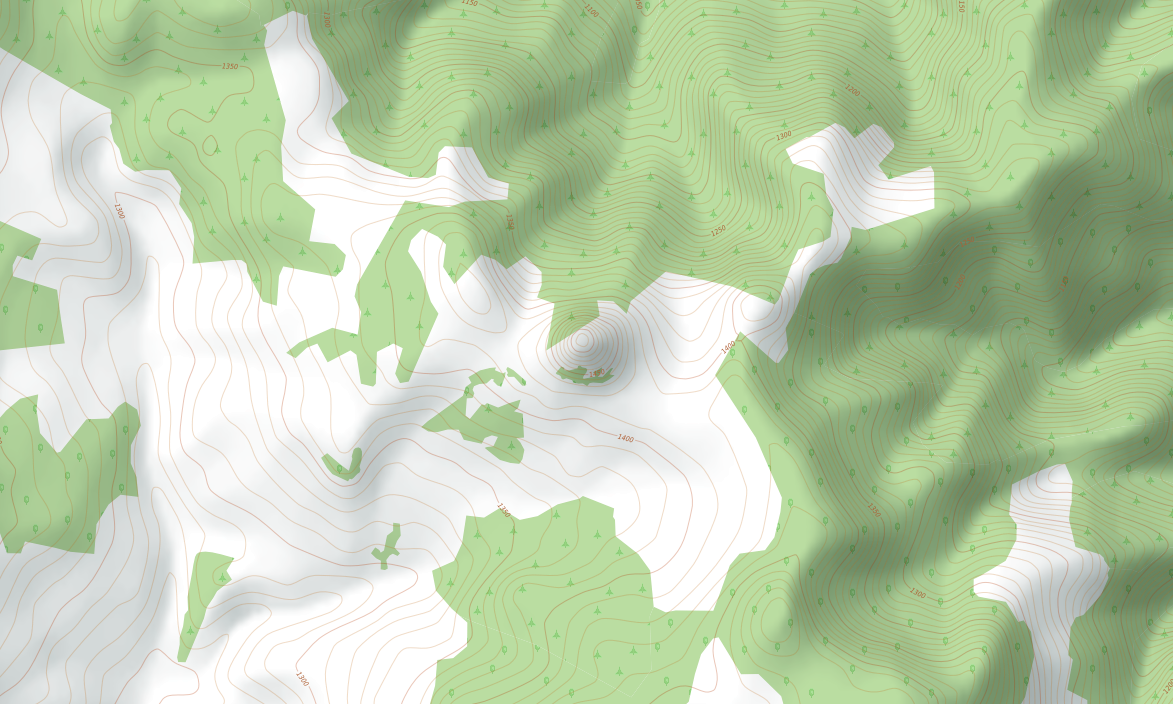
\includegraphics[scale=0.3]{figures/fig-fonctions-topo}
	\end{center}
	\begin{itemize}
		\item Ici, une carte \emph{Open Street Map} avec au centre le mont Gerbier de Jonc (source de la Loire, 1551 m). 
		\item Les lignes de niveau correspondent à des altitudes équidistantes de $10$ m (par exemple, pour $c=1400$, $c=1410$, $c=1420$\ldots).
		\item Lorsque les lignes de niveau sont très espacées, le terrain est plutôt plat ; lorsque les lignes sont rapprochées le terrain est pentu.
		\item Par définition, si on se promène en suivant une ligne de niveau, on reste toujours à la même altitude !
	\end{itemize}
\end{exemple}



\begin{exemple}{}{}
	Voici le graphe et les lignes de niveau de la fonction $f : \Rr^2 \to \Rr$ définie par
	$$f(x,y) = \frac{\sin(r^2-x)}{r}+1 \quad \text{ où } r = \sqrt{x^2+y^2}.$$
	
	\begin{center}
		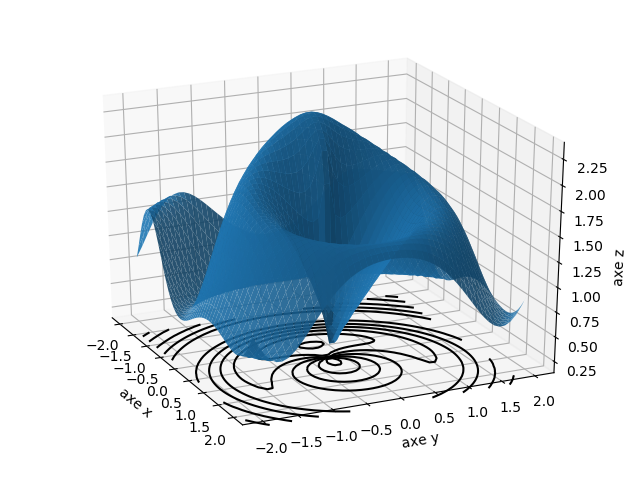
\includegraphics[scale=\myscale,scale=0.5]{figures/fonctions-niveau-2a}
		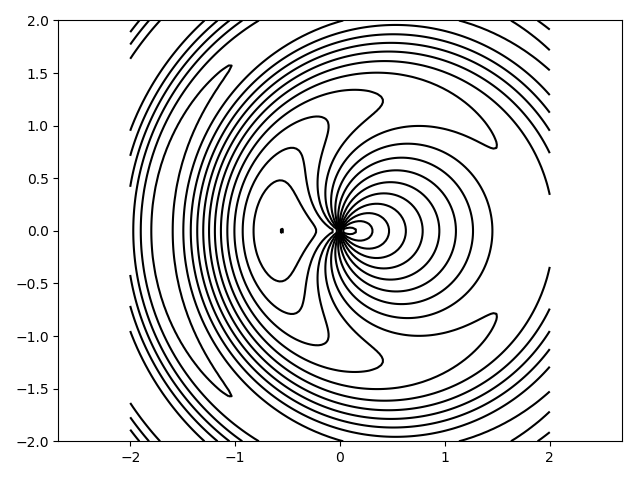
\includegraphics[scale=\myscale,scale=0.5]{figures/fonctions-niveau-2b}
	\end{center}
	% voir 'fonctions-niveau-2.py'
	
	
\end{exemple} 


%--------------------------------------------------------------------
\subsection{Surfaces quadratiques}

Ce sont des exemples à bien comprendre car ils seront importants pour la suite du cours.

\begin{exemple}{}{}
	$$f(x,y) = \frac{x^2}{a^2} + \frac{y^2}{b^2}-1$$
	
	
	
	\begin{itemize}
		\item Les tranches sont des paraboles.
		\item Les lignes de niveau sont des ellipses.
		\item Le graphe est donc un \trouer{paraboloïde elliptique}.
	\end{itemize}
	
	Ci-dessous : (a) la surface, (b) les tranches avec $x$ constant, (c) les tranches avec $y$ constant, (d) les courbes de niveau, (e) les lignes de niveau dans le plan.
	
	\begin{center}
		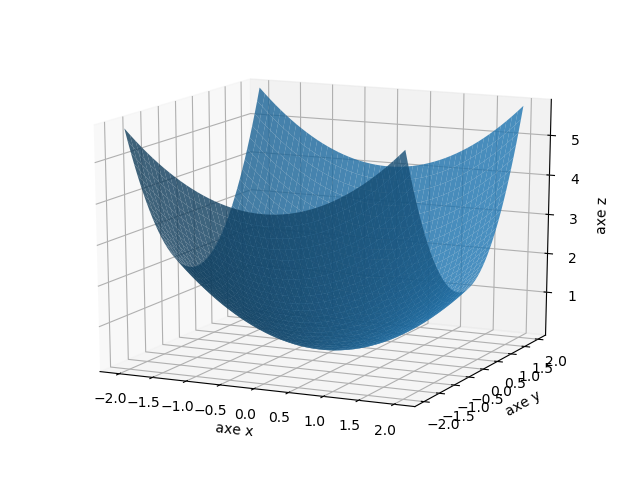
\includegraphics[scale=\myscale,scale=0.5]{figures/fonctions-quadra-1a}
		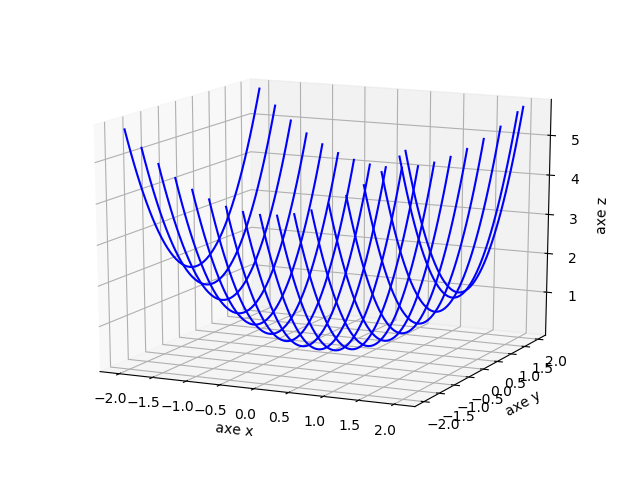
\includegraphics[scale=\myscale,scale=0.5]{figures/fonctions-quadra-1b}
		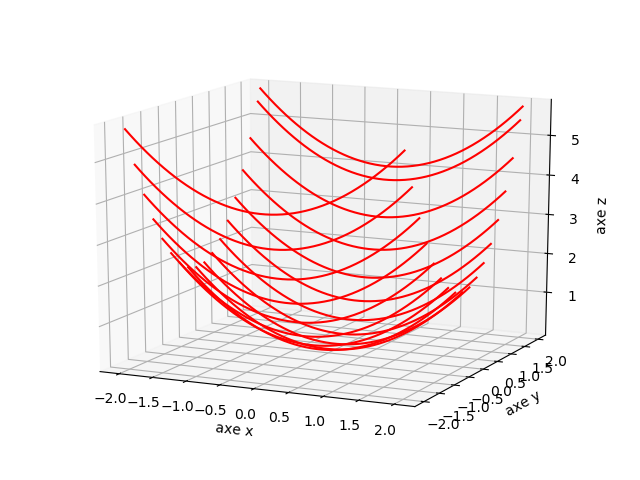
\includegraphics[scale=\myscale,scale=0.5]{figures/fonctions-quadra-1c}
		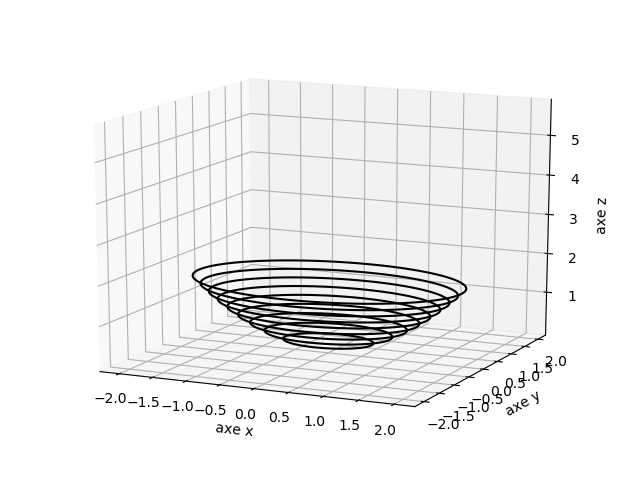
\includegraphics[scale=\myscale,scale=0.5]{figures/fonctions-quadra-1d}
		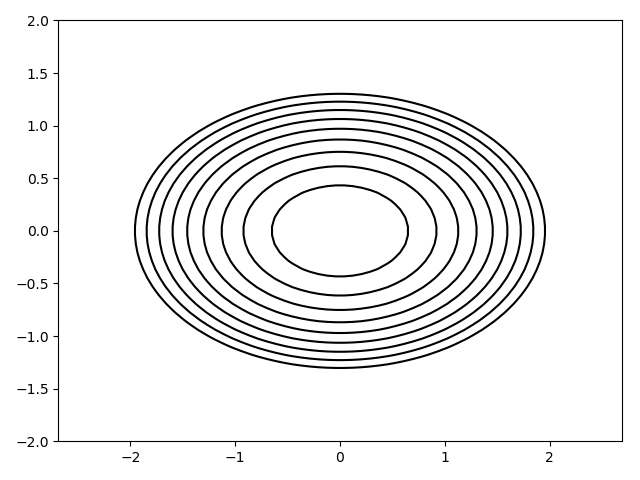
\includegraphics[scale=\myscale,scale=0.5]{figures/fonctions-quadra-1e}
	\end{center}
	
	% dessins 3d voir 'fonctions-quadra-1.py' 
	
\end{exemple}


\begin{exemple}{}{}
	$$f(x,y) = x^2$$
	
	
	
	\begin{itemize}
		\item Les tranches obtenues en coupant selon des plans $y=y_0$ sont des paraboles. Dans l'autre direction, ce sont des droites.
		\item Les lignes de niveau sont des droites.
		\item Le graphe est donc un \trouer{cylindre parabolique}.
	\end{itemize}
	
	Ci-dessous : (a) la surface, (b) les tranches avec $x$ constant, (c) les tranches avec $y$ constant, (d) les courbes de niveau, (e) les lignes de niveau dans le plan.
	\begin{center}
		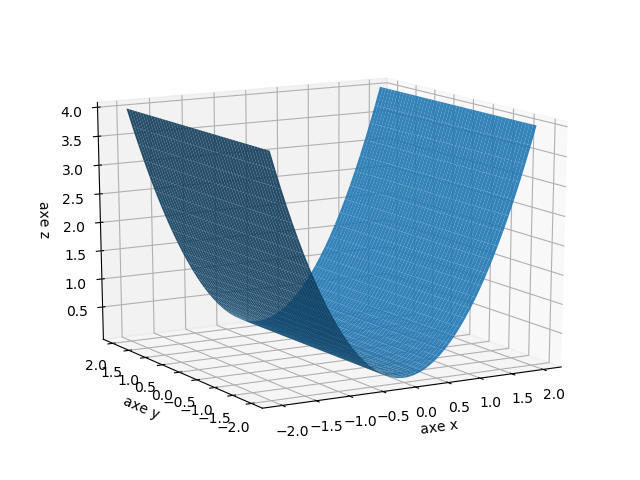
\includegraphics[scale=\myscale,scale=0.5]{figures/fonctions-quadra-2a}
		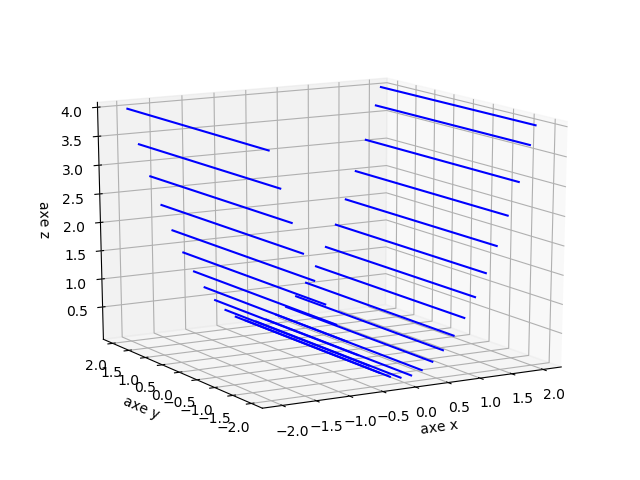
\includegraphics[scale=\myscale,scale=0.5]{figures/fonctions-quadra-2b}
		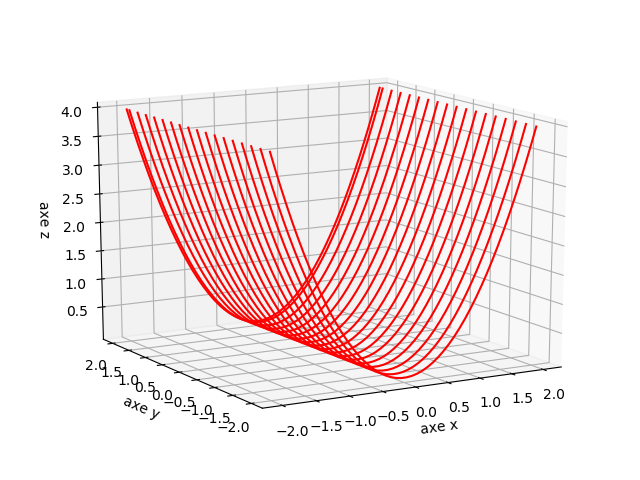
\includegraphics[scale=\myscale,scale=0.5]{figures/fonctions-quadra-2c}
		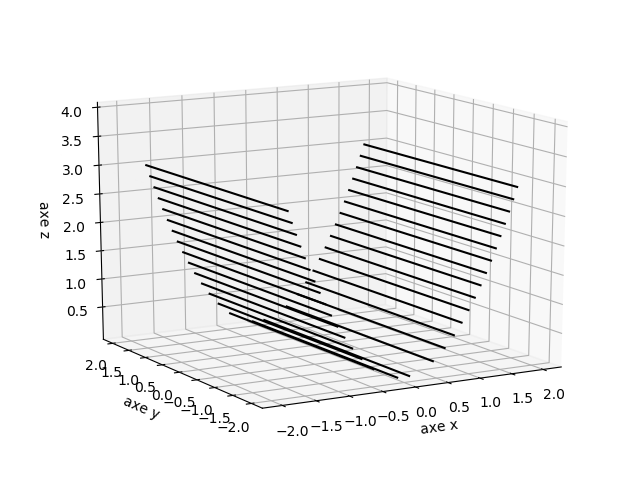
\includegraphics[scale=\myscale,scale=0.5]{figures/fonctions-quadra-2d}
		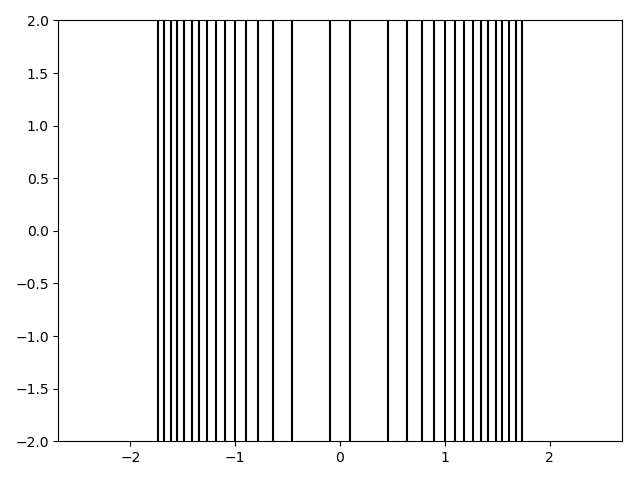
\includegraphics[scale=\myscale,scale=0.5]{figures/fonctions-quadra-2e}
	\end{center}
	
	% dessins 3d voir 'fonctions-quadra-2.py' 
	
	
\end{exemple}


\begin{exemple}{}{}
	$$f(x,y) = x^2-y^2$$
	
	
	\begin{itemize}
		\item Les tranches sont des paraboles, tournées vers le haut ou vers le bas selon la direction de la tranche.
		\item Les lignes de niveau sont des hyperboles.
		\item Le graphe est donc un \trouer{paraboloïde hyperbolique} que l'on appelle aussi la \trouer{selle de cheval}\index{point-selle}.
		\item Un autre nom pour cette surface est un \trouer{col} (en référence à un col en montagne). 
		En effet le point $(0,0,0)$, est le point de passage le moins haut pour passer d'un versant à l'autre de la montagne. 
	\end{itemize}
	
	Ci-dessous : (a) la surface, (b) les tranches avec $x$ constant, (c) les tranches avec $y$ constant, (d) les courbes de niveau, (e) les lignes de niveau dans le plan (en pointillé les lignes de niveau négatif).
	\begin{center}
		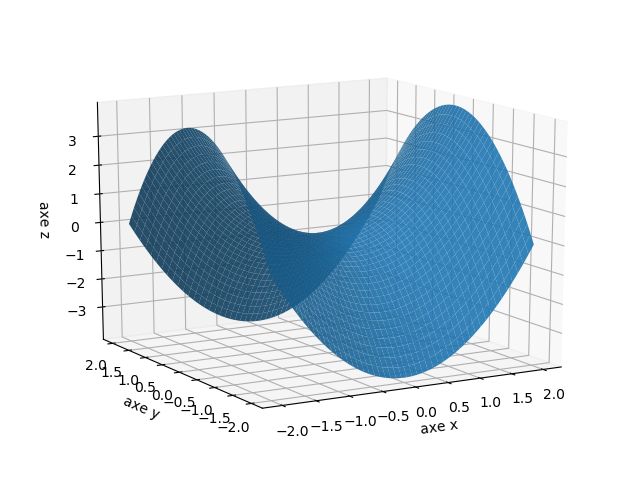
\includegraphics[scale=\myscale,scale=0.5]{figures/fonctions-quadra-3a}
		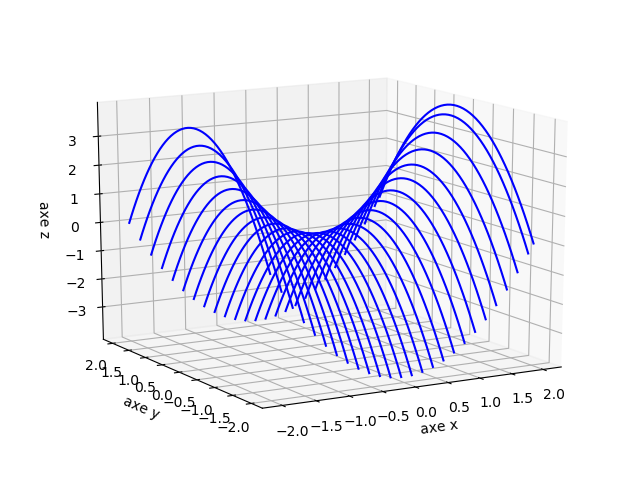
\includegraphics[scale=\myscale,scale=0.5]{figures/fonctions-quadra-3b}
		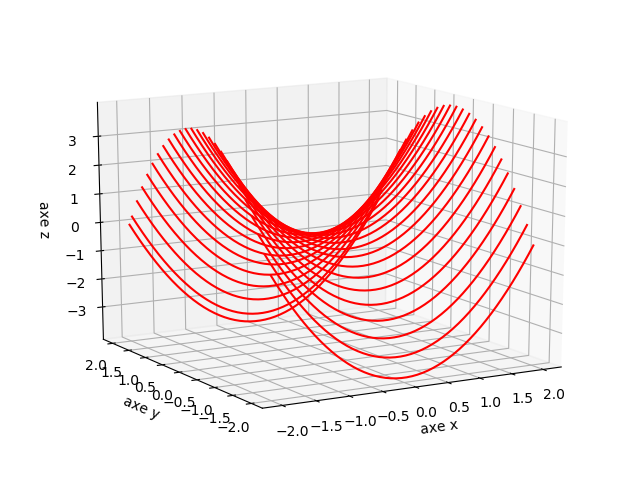
\includegraphics[scale=\myscale,scale=0.5]{figures/fonctions-quadra-3c}
		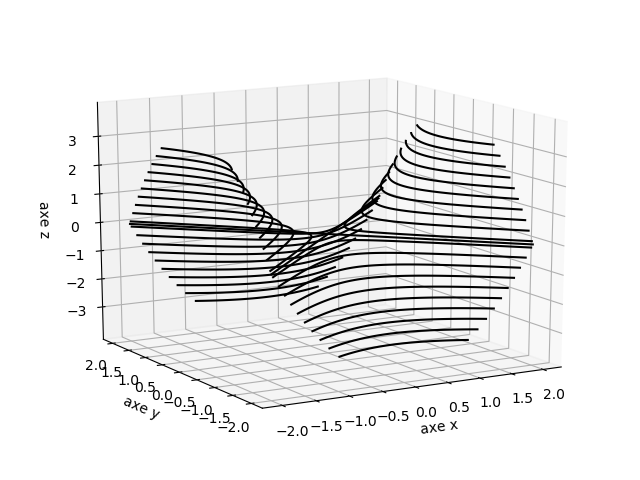
\includegraphics[scale=\myscale,scale=0.5]{figures/fonctions-quadra-3d}
		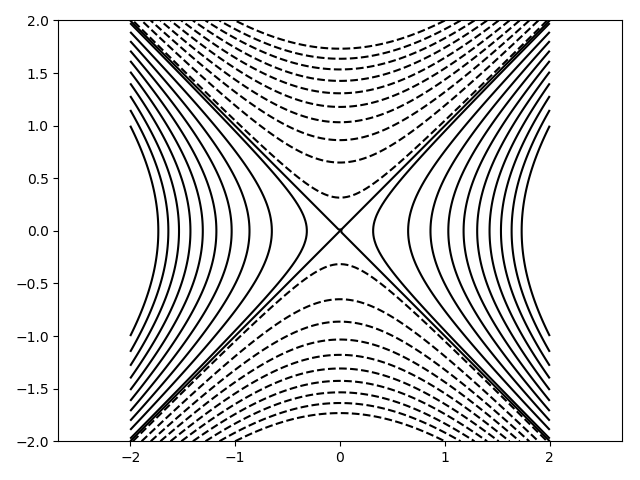
\includegraphics[scale=\myscale,scale=0.5]{figures/fonctions-quadra-3e}
	\end{center}
	
	% dessins 3d voir 'fonctions-quadra-3.py' 
\end{exemple}


%--------------------------------------------------------------------
\subsection{Régression linéaire}

\index{regression lineaire@régression linéaire}

\begin{exemple}{}{}
	On se donne des points du plan, comme ci-dessous. On s'aperçoit qu'ils sont à peu près alignés et on souhaite trouver l'équation d'une droite :
	$$y= a x + b$$ 
	qui les approche au mieux.
	
	
	\myfigure{0.6}{
		\tikzinput{fig-fonctions-10}
	}
	
	
	Formalisons un peu le problème : on se donne $N$ points $A_i(x_i,y_i)$, $i=1,\ldots,N$. Pour une droite $\mathcal{D}$ d'équation $y=ax+b$, la distance entre $A_i$ et la droite $\mathcal{D}$ est donnée par la formule :
	$$d(A_i,\mathcal{D}) = \frac{|ax_i-y_i+b|}{\sqrt{1+a^2}}.$$
	Pour se débarrasser des valeurs absolues et des racines carrées, on élève au carré et on décide que la droite qui approche au mieux tous les points $A_i$ est la droite qui minimise la fonction 
	$$f(a,b) = \sum_{i=1}^{N} d(A_i,\mathcal{D})^2 = 
	\frac{1}{1+a^2} \sum_{i=1}^{N}  (ax_i-y_i+b)^2.$$
	
	Pour les $5$ points du dessin initial : $A_1(2,3)$, $A_2(3,5)$, 
	$A_2(4,4)$, $A_4(5,6)$ et $A_5(6,6)$, il s'agit donc de trouver $(a,b)$ qui minimise la fonction 
	$$f(a,b) = \frac{1}{1+a^2} \left( 
	(2a-3+b)^2 + (3a-5+b)^2 + (4a-4+b)^2 + (5a-6+b)^2 + (6a-6+b)^2 \right).$$
	
	
	On trace le graphe de $f$, les lignes de niveau de $f$, et on utilise les techniques à notre disposition pour trouver qu'un minimum global est réalisé en $(a,b) \simeq (0.8,1.6)$, ce qui permet de tracer une droite $y=ax+b$ solution.
	
	\myfigure{0.6}{
		\tikzinput{fig-fonctions-11}
	} 
	
	Lorsque l'on dessine les lignes de niveau, on s'aperçoit que le minimum \couleurnb{(le point bleu) }{}se trouve dans une région plate et allongée. Cela signifie que, bien que le minimum $(a_{\min},b_{\min})$ soit unique, il existe beaucoup de $(a,b)$ tels que $f(a,b)$ soit proche de la valeur minimale $f(a_{\min},b_{\min})$. De plus, ces points $(a,b)$ peuvent être assez éloignés de la solution $(a_{\min},b_{\min})$ (par exemple tous les points de la zone ovale autour du \couleurnb{point bleu}{minimum}). Ce qui signifie que beaucoup de droites très différentes approchent la solution optimale.
	
	
	\begin{center}
		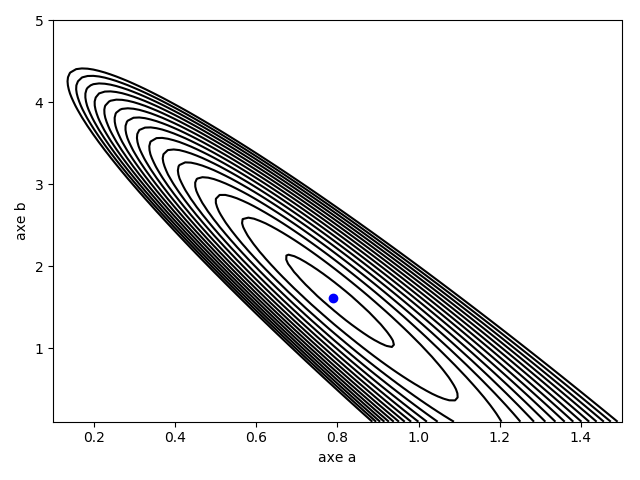
\includegraphics[scale=\myscale,scale=0.7]{figures/fonctions-regression}
	\end{center}
	% voir 'fonctions-regression-1.py'
	
\end{exemple}

%\objectifs{}



%%%%%%%%%%%%%%%%%%%%%%%%%%%%%%%%%%%%%%%%%%%%%%%%%%%%%
\section{Dérivées partielles}

Pour une fonction de plusieurs variables, il existe une dérivée pour chacune des variables, qu'on appelle dérivée partielle. 

%----------------------------------------------------
\subsection{Définition}


\begin{definition}{}{}
	Soit $f : \Rr^2 \to \Rr$. 
	La \trouer{dérivée partielle}\index{derivee partielle@dérivée partielle} $\frac{\partial f}{\partial x} (x_0,y_0)$ de $f$ par rapport à la variable $x$ au point $(x_0,y_0) \in \Rr^2$ est la dérivée en $x_0$ de 
	la fonction d'une variable $x \mapsto f(x, y_0)$.
	
	De même $\frac{\partial f}{\partial y} (x_0,y_0)$ est la dérivée partielle de $f$ par rapport à la variable $y$ au point $(x_0,y_0)$.
	
	
\end{definition}

Comme d'habitude et sauf mention contraire, nous supposerons que toutes les dérivées partielles existent.

Autrement dit, en revenant à la définition de la dérivée comme une limite :
$$\frac{\partial f}{\partial x} (x_0,y_0) = \lim_{h \rightarrow 0} 
\frac{f(x_0+h, y_0) - f(x_0,y_0)}{h}
\quad \text{ et } \quad 
\frac{\partial f}{\partial y} (x_0,y_0) = \lim_{h \rightarrow 0} 
\frac{f(x_0, y_0+h) - f(x_0,y_0)}{h}.$$




Plus généralement, pour une fonction $f : \Rr^n \to \Rr$ de plusieurs variables,
$\frac{\partial f}{\partial x_i} (x_1,\ldots,x_n)$ est la dérivée partielle de $f$ par rapport à la variable $x_i$ au point $(x_1,\ldots,x_n) \in \Rr^n$.
C'est la dérivée en $x_i$ de la fonction d'une variable $x_i \mapsto f(x_1,\ldots,x_n)$ où l'on considère fixes les variables $x_j$ pour $j \neq i$.

\bigskip

\textbf{Notations.}
$$\frac{\partial f}{\partial x} (x,y) \quad \text{ et } \quad \frac{\partial f}{\partial y} (x,y)$$
sont les analogues de l'écriture $\frac{\dd f}{\dd x}(x)$ pour l'écriture de la dérivée lorsqu'il n'y a qu'une seule variable.
Le symbole \og{}$\partial$\fg{} se lit \og{}d rond\fg{}.
Une autre notation est $\partial_x f(x,y)$, $\partial_y f(x,y)$ ou bien encore $f'_x (x,y)$, $f'_y (x,y)$.


%----------------------------------------------------
\subsection{Calculs}

La calcul d'une dérivée partielle n'est pas plus compliqué que le calcul d'une dérivée.

\textbf{Méthode.}
Pour calculer une dérivée partielle par rapport à une variable, il suffit de dériver par rapport à cette variable en considérant les autres variables comme des constantes.


\begin{exemple}{}{}
	Calculer les dérivées partielles de la fonction 
	$f : \Rr^2 \to \Rr$ définie par $f(x,y)=x^2e^{3y}$.
	
	\medskip
	\emph{Solution.}
	
	Pour calculer la dérivée partielle $\frac{\partial f}{\partial x}$, par rapport à $x$, on considère que $y$ est une constante et on dérive $x^2e ^{3y}$ comme si c'était une fonction de la variable $x$ uniquement :
	$$\frac{\partial f}{\partial x}(x,y) =2xe ^{3y}.$$
	Pour l'autre dérivée  $\frac{\partial f}{\partial y}$, on considère que $x$ est une constante et on dérive $x^2e ^{3y}$ comme si c'était une fonction de $y$ :
	$$\frac{\partial f}{\partial y}(x,y) = 3x^2e ^{3y}.$$
\end{exemple}



\begin{exemple}{}{}
	Pour $f : \Rr^3 \to \Rr$ définie par $f(x,y,z)=\cos (x+y^2)e^{-z}$ on a :
	\begin{align*}
		\frac{\partial f}{\partial x}(x,y,z) = -\sin(x+y^2)e^{-z}, \\
		\frac{\partial f}{\partial y}(x,y,z) = -2y\sin(x+y^2)e^{-z}, \\
		\frac{\partial f}{\partial z}(x,y,z) = -\cos(x+y^2)e^{-z}.
	\end{align*}
\end{exemple}


\begin{exemple}{}{}
	Soit $f :\Rr^n \to \Rr$ définie par 
	$f(x_1,\ldots,x_n) = x_1^2+x_2^2+\cdots + x_n^2$,
	alors pour $i=1,\ldots,n$ :
	$$\frac{\partial f}{\partial x_i}(x_1,\ldots,x_n) = 2x_i.$$
\end{exemple}


%----------------------------------------------------
\subsection{Interprétation géométrique}


Pour une fonction d'une variable, la dérivée est la pente de la tangente au graphe de la fonction (le graphe étant alors une courbe). Pour une fonction de deux variables $(x,y) \mapsto f(x,y)$, les dérivées partielles indiquent les pentes au graphe de $f$ selon certaines directions (le graphe étant ici une surface). Plus précisément :

\begin{itemize}
	\item $\frac{\partial f}{\partial x} (x_0,y_0)$ est la pente du graphe de $f$
	en $(x_0,y_0)$ suivant la direction de l'axe $(Ox)$.
	En effet cette pente est celle de la tangente à la courbe $z = f(x,y_0)$ et est donnée par la dérivée de $x \mapsto f(x,y_0)$ en $x_0$, c'est donc bien $\frac{\partial f}{\partial x} (x_0,y_0)$.
	
	\item $\frac{\partial f}{\partial y} (x_0,y_0)$ est la pente du graphe de $f$
	en $(x_0,y_0)$ suivant la direction de l'axe $(Oy)$.
	
	
\end{itemize}



\bigskip 
Sur la figure de gauche, la dérivée partielle  $\frac{\partial f}{\partial x}$ indique la pente de la tranche parallèle à l'axe $(Ox)$\couleurnb{ (en orange)}{}. Sur la figure de droite, la dérivée partielle  $\frac{\partial f}{\partial y}$ indique la pente de la tranche parallèle à l'axe $(Oy)$\couleurnb{ (en vert)}{}.


\myfigure{0.75}{
	\tikzinput{fig-calculdiff-04}
	\tikzinput{fig-calculdiff-05}
} 





%%%%%%%%%%%%%%%%%%%%%%%%%%%%%%%%%%%%%%%%%%%%%%%%%%%%%
\section{Gradient}

Le gradient est un vecteur dont les coordonnées sont les dérivées partielles. Il a de nombreuses applications géométriques car il donne l'équation des tangences aux courbes et surfaces de niveau. Surtout, il indique la direction dans laquelle la fonction varie le plus vite.

Le gradient est un vecteur qui remplace la notion de dérivée pour les fonctions de plusieurs variables. On sait que la dérivée permet de décider si une fonction est croissante ou décroissante. De même, le vecteur gradient indique la direction dans laquelle la fonction croît ou décroît le plus vite. Nous allons voir comment calculer de façon algorithmique le gradient grâce à la \og{}différentiation automatique\fg{}.

%----------------------------------------------------
\subsection{Définition}

\begin{definition}{}{}
	Soit $f : \Rr^2 \to \Rr$ une fonction admettant des dérivées partielles.
	Le \trouer{gradient}\index{gradient} de $f$ en $(x_0,y_0) \in \Rr^2$, noté 
	$\grad f (x_0,y_0)$, est le vecteur :
	$$\grad f (x_0,y_0) =
	\begin{pmatrix} \dfrac{\partial f}{\partial x} (x_0,y_0)\\[2ex] \dfrac{\partial f}{\partial y}(x_0,y_0)\end{pmatrix}.$$
\end{definition}

Les physiciens et les anglo-saxons notent souvent $\nabla f (x,y)$ pour $\grad f (x,y)$. Le symbole $\nabla$ se lit \og{}nabla\fg{}.


Plus généralement, pour $f : \Rr^n \to \Rr$, le gradient de $f$ en $(x_1,\ldots,x_n) \in \Rr^n$ est le vecteur :
$$\grad f (x_1,\ldots,x_n) =
\begin{pmatrix} \dfrac{\partial f}{\partial x_{1}} (x_1,\ldots,x_n)\\ \vdots \\ \dfrac{\partial f}{\partial x_n}(x_1,\ldots,x_n)\end{pmatrix}.$$



\begin{exemple}{}{}
	\begin{itemize}
		\item $f(x,y) = x^2y^3$, $\grad f (x,y) =  \begin{pmatrix}2xy^3\\3x^2y^2\end{pmatrix}$. Au point $(x_0,y_0)=(2,1)$, $\grad f (2,1) =  \begin{pmatrix}4\\12\end{pmatrix}$.
		
		\item $f(x,y,z) = x^2\sin(yz)$, $\grad f (x,y,z) = \begin{pmatrix} 2x\sin(yz) \\ x^2z \cos(yz) \\ x^2y\cos(yz) \end{pmatrix}$.
		
		\item $f(x_1,\ldots,x_n)= x_1^2+x_2^2+\cdots + x_n^2$, $\grad f (x_1,\ldots,x_n) =  \begin{pmatrix}2x_1\\ \vdots \\2x_n\end{pmatrix}$.
	\end{itemize}
\end{exemple}



%----------------------------------------------------
\subsection{Tangentes aux lignes de niveau}


Soit $f : \Rr^2 \to \Rr$ une fonction différentiable. On considère les lignes de niveau $f(x,y)=k$.


\begin{proposition}{}{}
	\index{lignes de niveau}
	Le vecteur gradient $\grad f(x_0,y_0)$ est orthogonal à la ligne de niveau de $f$ passant au point $(x_0,y_0)$. 
\end{proposition}


Sur ce premier dessin, sont dessinés la ligne de niveau passant par le point $(x_0,y_0)$ \couleurnb{(en rouge)}{}, un vecteur tangent $v$ en ce point et la tangente à la ligne de niveau\couleurnb{ (en vert)}{}. 
Le vecteur gradient est un vecteur du plan qui est orthogonal à la ligne de niveau en ce point\couleurnb{ (en bleu)}{}.


\bigskip

\myfigure{0.8}{
	\tikzinput{fig-gradient-02}
}

À chaque point du plan, on peut associer un vecteur gradient. Ce vecteur gradient est orthogonal à la ligne de niveau passant par ce point. Nous verrons juste après comment savoir s'il est orienté \og{}vers le haut\fg{} ou \og{}vers le bas\fg{}. 

\myfigure{0.8}{
	\tikzinput{fig-gradient-01}
}

Dans le cadre de notre étude, nous nous intéressons à l'équation de la tangente.
\begin{proposition}{}{}
	\index{tangente}
	Au point $(x_0,y_0)$, l'équation de la tangente à la ligne de niveau de $f$ est :
	$$\frac{\partial f}{\partial x}(x_0,y_0)(x-x_0)+\frac{\partial f}{\partial y}(x_0,y_0)(y-y_0)=0$$
	pourvu que le gradient de $f$ en ce point ne soit pas le vecteur nul.
\end{proposition}



\begin{exemple}{Tangentes à une ellipse}{}
	Trouver les tangentes à l'ellipse $\mathcal{E}$ d'équation $\frac{x^2}{a^2}+\frac{y^2}{b^2} = 1$.
	
	\myfigure{0.7}{
		\tikzinput{fig-gradient-03}
	}
	
	Cette ellipse $\mathcal{E}$ est la ligne de niveau $f(x,y)=1$ de la fonction
	$f(x,y) = \frac{x^2}{a^2}+\frac{y^2}{b^2}$. 
	Les dérivées partielles en $(x_0, y_0)$ sont :
	$$\frac{\partial f}{\partial x}(x_0,y_0) = \frac{2x_0}{a^2} \qquad \text{ et } \qquad \frac{\partial f}{\partial y}(x_0,y_0) = \frac{2y_0}{b^2}.$$
	L'équation de la tangente à l'ellipse $\mathcal{E}$ en ce point est donc :
	$$\frac{2x_0}{a^2}(x-x_0)+\frac{2y_0}{b^2}(y-y_0)=0.$$
	Mais comme $\frac{x_0^2}{a^2}+\frac{y_0^2}{b^2} = 1$, l'équation de la tangente se simplifie en $\displaystyle \frac{x_0}{a^2}x + \frac{y_0}{b^2} y = 1$.
\end{exemple}


%----------------------------------------------------
\subsection{Lignes de plus forte pente}

Considérons les lignes de niveau $f(x,y)=k$ d'une fonction $f : \Rr^2 \to \Rr$.
On se place en un point $(x_0,y_0)$. On cherche dans quelle direction se déplacer pour augmenter au plus vite la valeur de $f$.

\begin{proposition}{}{}
	Le vecteur gradient $\grad f(x_0,y_0)$ indique la direction de plus grande pente à partir du point $(x_0,y_0)$.
\end{proposition}


Autrement dit, si l'on veut, à partir d'un point donné $(x_0,y_0)$ de niveau $a$, passer au niveau $b>a$ le plus vite possible alors il faut démarrer en suivant la direction du gradient $\grad f(x_0,y_0)$. 

\myfigure{1}{
	\tikzinput{fig-gradient-05}
}

Comme illustration, un skieur de descente, voulant optimiser sa course, choisira en permanence de s'orienter suivant la plus forte pente, c'est-à-dire dans le sens opposé au gradient. 

%----------------------------------------------------
\subsection{Dérivée directionnelle}

Pour prouver que le gradient indique la ligne de la plus grande pente, nous avons besoin de généraliser la notion de dérivée partielle. Ce passage est plus technique et peut être ignoré en première lecture.

Soit $v=\left(\begin{smallmatrix}h\\k\end{smallmatrix}\right)$ un vecteur du plan.
La \trouer{dérivée directionnelle} de $f$ suivant le vecteur $v$ en $(x_0,y_0)$ est le nombre :
$$D_v f(x_0,y_0) = h\frac{\partial f}{\partial x}(x_0,y_0)
+k\frac{\partial f}{\partial y}(x_0,y_0).$$


La dérivée directionnelle correspond à la pente de la fonction pour la tranche dirigée par le vecteur $v$.

\myfigure{0.8}{
	\tikzinput{fig-calculdiff-06}
} 

Remarque : pour $v=\left(\begin{smallmatrix}1\\0\end{smallmatrix}\right)$
alors $D_v f(x_0,y_0) = \frac{\partial f}{\partial x}(x_0,y_0)$ et pour 
$v=\left(\begin{smallmatrix}0\\1\end{smallmatrix}\right)$
alors $D_v f(x_0,y_0) = \frac{\partial f}{\partial y}(x_0,y_0)$.


On rappelle que le \trouer{produit scalaire} de deux vecteurs $u=\left(\begin{smallmatrix}x\\y\end{smallmatrix}\right)$ et 
$v=\left(\begin{smallmatrix}x'\\y'\end{smallmatrix}\right)$
est donné par 
$$\langle u \mid v \rangle = xx' + yy'.$$
On sait que le produit scalaire se calcule aussi géométriquement par :
$$\langle u \mid v \rangle = \|u\|\cdot \|v\| \cdot \cos(\theta)$$
où $\theta$ est l'angle entre $u$ et $v$.

\myfigure{1}{
	\tikzinput{fig-scalaire}
} 


Ainsi, on peut réécrire la dérivée directionnelle sous la forme :
$$D_v f(x_0,y_0) = \langle \grad f (x_0,y_0) \mid v \rangle.$$


On peut maintenant prouver que le gradient indique la ligne de plus grande pente.

\begin{proof}
	La dérivée suivant le vecteur non nul $v$ au point $(x_0,y_0)$ décrit la variation de $f$ autour de ce point lorsqu'on se déplace dans la direction $v$. 
	La direction selon laquelle la croissance est la plus grande est celle du gradient de $f$. En effet,
	$$D_{v}f(x_0,y_0)=\langle \grad f(x_0,y_0) \mid v\rangle=
	\| \grad f(x_0,y_0) \| \cdot \| v \| \cdot \cos \theta$$
	où $\theta$ est l'angle entre le vecteur $\grad f(x_0,y_0)$ et le vecteur $v$.
	Le maximum est atteint lorsque l'angle $\theta=0$, c'est-à-dire lorsque $v$ pointe dans la même direction que $\grad f(x_0,y_0)$.
\end{proof}


%----------------------------------------------------
\subsection{Surface de niveau}

Les résultats présentés ci-dessus pour les fonctions de deux variables se généralisent aux fonctions de trois variables ou plus.
Commençons avec trois variables et une fonction $f:\Rr^3 \to \Rr$.
Rappelons qu'un plan de $\Rr^3$ passant par $(x_0,y_0,z_0)$ et de vecteur normal 
$n=(a,b,c)$ a pour équation cartésienne :
$$a(x-x_0)+b(y-y_0)+c(z-z_0) = 0.$$


De même qu'il existe une droite tangente pour les lignes de niveau, il existe un \trouer{plan tangent} à une surface de niveau.


\begin{proposition}{}{}
	Le vecteur gradient $\grad f(x_0,y_0,z_0)$ est orthogonal à la surface de niveau de $f$ passant au point $(x_0,y_0,z_0)$. Autrement dit,
	l'équation du plan tangent à la surface de niveau de $f$ en $(x_0,y_0,z_0)$ est 
	$$\frac{\partial f}{\partial x}(x_0,y_0,z_0)(x-x_0)
	+\frac{\partial f}{\partial y}(x_0,y_0,z_0)(y-y_0)
	+\frac{\partial f}{\partial z}(x_0,y_0,z_0)(z-z_0)
	= 0 $$
	pourvu que le gradient de $f$ en ce point ne soit pas le vecteur nul.
\end{proposition}


\myfigure{1}{
	\tikzinput{fig-gradient-07}
}


Plus généralement pour $f : \Rr^n \to \Rr$, $\grad f (x_1,\ldots,x_n)$ est orthogonal à l'espace tangent à
l'hypersurface de niveau $f=k$ passant par le point $(x_1,\ldots,x_n)\in\Rr^n$ et 
ce vecteur gradient $\grad f(x_1,\ldots,x_n)$ indique la direction de plus grande pente à partir du point $(x_1,\ldots,x_n)$.



%----------------------------------------------------
\subsection{Calcul approché}

Rappelez-vous que la dérivée nous a permis de faire des calculs approchés, par exemple pour estimer $\sqrt{1.01}$ sans calculatrice (voir le chapitre \og{}Dérivée\fg{}).
Voici, en deux variables, l'analogue de la formule pour une variable : 
$$f(x_0+h,y_0+k) \simeq f(x_0,y_0) + h\frac{\partial f}{\partial x}(x_0,y_0)
+k\frac{\partial f}{\partial y}(x_0,y_0).$$
Cette approximation est valable pour $h$ et $k$ petits.

L'interprétation géométrique est la suivante : 
on approche le graphe de $f$ en $(x_0,y_0)$ par le plan tangent au graphe en ce point. Sur la figure ci-dessous sont représentés : le graphe de $f$\couleurnb{ (en rouge)}{}, le plan tangent au-dessus du point $(x_0,y_0)$\couleurnb{ (en bleu)}{}. La valeur $z_1 = f(x_0+h,y_0+k)$ est la valeur exacte donnée par le point de la surface au dessus de $(x_0+h,y_0+k)$. On approche cette valeur par $z_2 = f(x_0,y_0) + h\frac{\partial f}{\partial x}(x_0,y_0)
+k\frac{\partial f}{\partial y}(x_0,y_0)$ donnée par le point du plan tangent au dessus de $(x_0+h,y_0+k)$. 


\myfigure{1}{
	\tikzinput{fig-gradient-10}
}


\begin{exemple}{}{}
	Valeur approchée de $f(1.002, 0.997)$ si $f(x,y) = x^2y$.
	\bigskip
	
	\emph{Solution.}
	Ici $(x_0,y_0) = (1,1)$, $h = 2 \times 10^{-3}$, $k = -3 \times 10^{-3}$,
	$\frac{\partial f}{\partial x}(x,y) = 2xy$, $\frac{\partial f}{\partial y}(x,y) = x^2$, donc $\frac{\partial f}{\partial x}(x_0,y_0) = 2$, $\frac{\partial f}{\partial y}(x_0,y_0) = 1$. Ainsi
	$$f(1+h,1+k) \simeq f(1,1) + 2h + k$$
	donc 
	$$f(1.002, 0.997) \simeq 1 + 2 \times 2 \times 10^{-3} - 3 \times 10^{-3} \simeq 1.001.$$
	Avec une calculatrice, on trouve $f(1.002, 0.997) = 1.000992$ : l'approximation est bonne.
\end{exemple}


%----------------------------------------------------
\subsection{Minimum et maximum}

\begin{definition}{}{}
	\index{minimum!local}
	Soit $f : \Rr^2 \to \Rr$.
	\begin{itemize}
		\item La fonction $f$ admet un \trouer{minimum local} en $(x_0,y_0)$ s'il existe un disque $D$ centré en ce point tel que 
		$$ f(x,y) \ge f(x_0,y_0) \quad \text{ pour tout } (x,y) \in D.$$
		\item La fonction $f$ admet un \trouer{maximum local} en $(x_0,y_0)$  pour lequel 
		$$f(x,y) \le f(x_0,y_0) \quad \text{ pour tout } (x,y) \in D.$$
		\item On parle d'un \trouer{extremum local} pour un minimum ou un maximum local.
	\end{itemize}
\end{definition}

% [[dessins 3D min/max]]

\begin{exemple}{}{}
	L'exemple type de minimum est celui de la fonction $f(x,y)=x^2+y^2$ en $(0,0)$.
	Voici son graphe et ses lignes de niveau.
	
	\begin{center}
		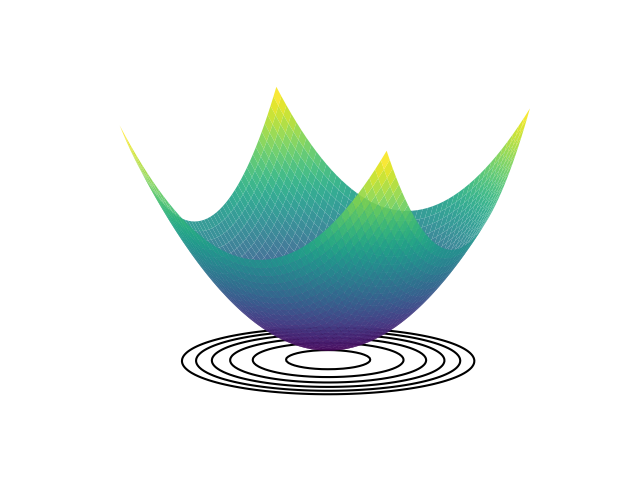
\includegraphics[scale=\myscale,scale=0.7]{figures/gradient-surface-1a}
	\end{center}
	
	
	La fonction $f(x,y) = -x^2-y^2$ admet, elle, un maximum en $(0,0)$.
	\begin{center}
		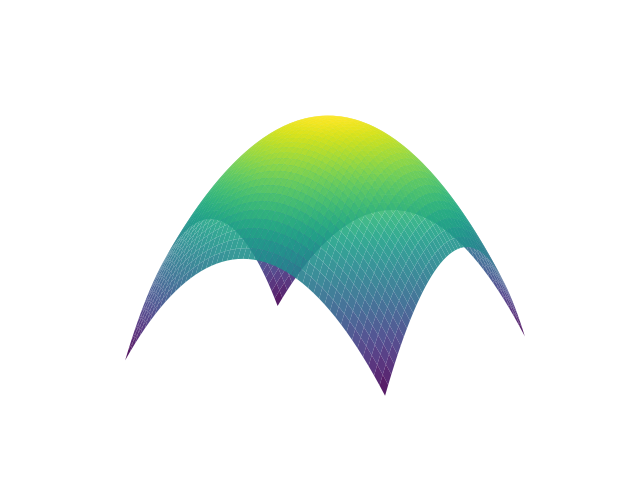
\includegraphics[scale=\myscale,scale=0.7]{figures/gradient-surface-2}
	\end{center}
	
\end{exemple}

\begin{proposition}{}{}
	Soit $f : \Rr^2 \to \Rr$. Si $f$ admet un minimum ou un maximum local en $(x_0,y_0)$ alors le gradient est le vecteur nul en ce point, autrement dit :
	$$
	\frac{\partial f}{\partial x}(x_0,y_0) = 0 
	\quad \text{ et  }\quad
	\frac{\partial f}{\partial y}(x_0,y_0) = 0.
	$$
\end{proposition}

\begin{proof}
	Prenons le cas d'un minimum local.
	La fonction d'une variable $x \mapsto f(x, y_0)$ admet aussi un minimum en $x_0$ donc sa dérivée est nulle en $x_0$, c'est-à-dire $\frac{\partial f}{\partial x}(x_0,y_0) = 0$. De même $y \mapsto f(x_0, y)$ admet un minimum en $y_0$ donc $\frac{\partial f}{\partial y}(x_0,y_0) = 0$. 
\end{proof}


Dans la suite du cours nous chercherons les points pour lesquels une fonction donnée présente un minimum local.
D'après la proposition précédente, ces points sont à chercher parmi les points en lesquels le gradient s'annule. On dira que $(x_0,y_0)$ est un \trouer{point critique}\index{point critique} de $f$ si
les deux dérivées partielles $\frac{\partial f}{\partial x}(x_0,y_0)$ et $\frac{\partial f}{\partial y}(x_0,y_0)$ s'annulent simultanément.

\begin{definition}{points stationnaires / critiques}{}
	Un point stationnaires (ou point critique) d'une fonction $f : \Rr^2 \to \Rr$ est un point $(x_0,y_0)$ en lequel le gradient s'annule, c'est-à-dire : 
	$$\frac{\partial f}{\partial x}(x_0,y_0) = 0
	\quad \text{ et } \quad
	\frac{\partial f}{\partial y}(x_0,y_0) = 0.$$
\end{definition}

\begin{exemple}{}{}
	Chercher les points en lesquels $f(x,y) = x^2-y^3+xy$ peut atteindre son minimum.
	
	\textbf{Recherche des points critiques.}
	On calcule 
	$$\frac{\partial f}{\partial x}(x,y) = 2x+y 
	\quad \text{ et } \quad 
	\frac{\partial f}{\partial y}(x,y) = -3y^2+x.$$
	On cherche les points $(x,y)$ en lesquels les deux dérivées partielles s'annulent.
	Par l'annulation de la première dérivée, on a $2x+y=0$ donc $y=-2x$.
	Par l'annulation de la seconde dérivée, on a $-3y^2+x=0$ ce qui donne par substitution
	$-12x^2+x=0$, ainsi $x(-12x+1)=0$.
	Donc soit $x=0$ et alors on a $y=0$, soit $x=\frac1{12}$ et alors $y=-\frac16$.
	Bilan : il y a deux points critiques :
	$$\left(0,0\right) \quad \text{ et } \quad \left(\frac1{12},-\frac16\right).$$
	
	\textbf{\'Etude du point critique $(0,0)$.}
	On a $f(0,0)=0$ mais on remarque que $f(0,y)=-y^3$ qui peut être négatif ou positif (selon le signe de $y$ proche de $0$), donc en $(0,0)$ il n'y a ni minimum ni maximum.
	
	\textbf{\'Etude du point critique $(\frac1{12},-\frac16)$.}
	Il existe un critère (que l'on ne décrira pas ici) qui permet de dire qu'en ce point $f$ admet un minimum local.
	
	Sur le dessin ci-dessous, le minimum est situé à l'intérieur du petit ovale, l'autre point critique en $(0,0)$ correspond à l'intersection de la ligne de niveau $f=0$ avec elle-même.
	\begin{center}
		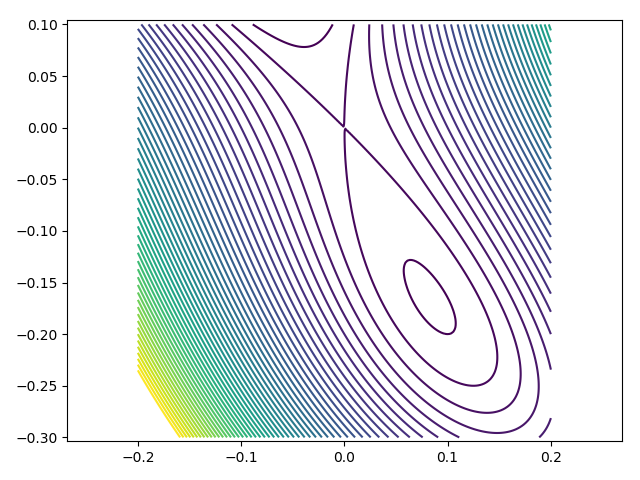
\includegraphics[scale=\myscale,scale=0.7]{figures/gradient-surface-6}
	\end{center}
	
\end{exemple}
Sur l'exemple précédent, nous avons assez facilement calculé les points critiques à partir des deux équations à deux inconnues. Il faut prendre garde que ce n'est pas un système linéaire et que dans le cas d'une fonction plus compliquée il aurait été impossible de déterminer exactement les points critiques.

On note aussi dans l'exemple précédent que certains points critiques ne sont ni des maximums ni des minimums. L'exemple type, illustré ci-dessous, est celui d'un \trouer{col} appelé aussi \trouer{point-selle}\index{point-selle} en référence à sa forme de selle de cheval.

\begin{exemple}{}{}
	Soit $f(x,y)=x^2-y^2$.
	Voici son graphe vu sous trois angles différents et ses lignes de niveau.
	
	\begin{center}
		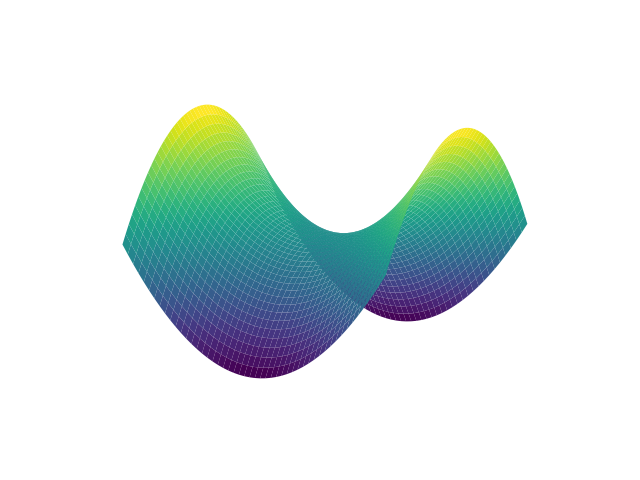
\includegraphics[scale=\myscale,scale=0.7]{figures/gradient-surface-3a}
	\end{center}
	\begin{center}
		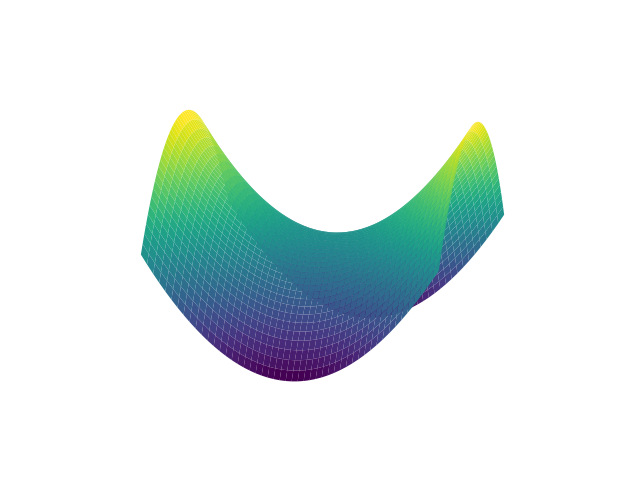
\includegraphics[scale=\myscale,scale=0.5]{figures/gradient-surface-3b}
		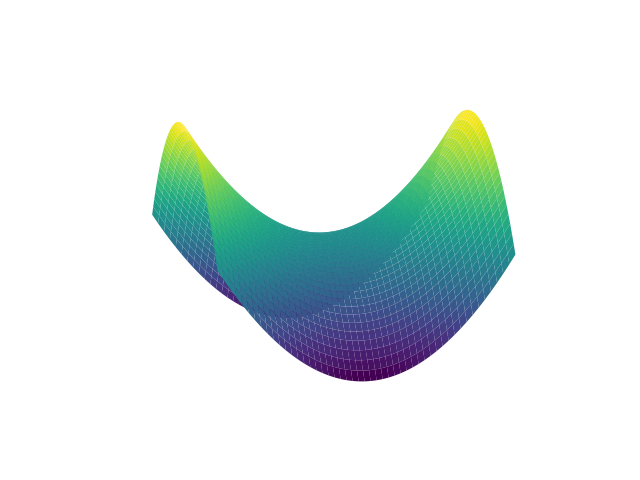
\includegraphics[scale=\myscale,scale=0.5]{figures/gradient-surface-3c}
	\end{center}
	\begin{center}
		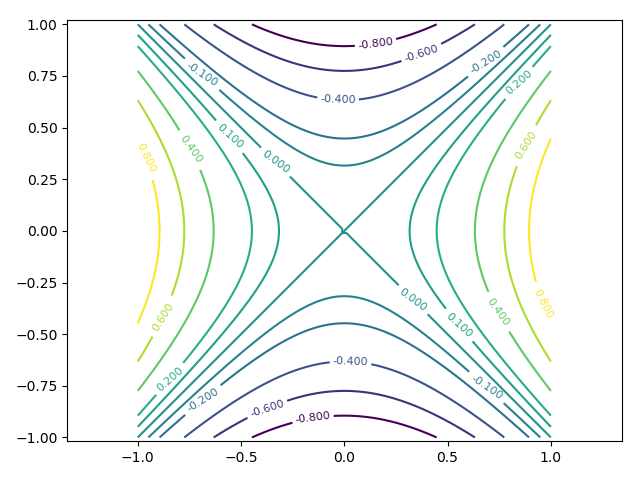
\includegraphics[scale=\myscale,scale=0.7]{figures/gradient-surface-4}
	\end{center}
	
	
\end{exemple}


Comme il peut être difficile de calculer les points critiques de façon exacte, nous allons utiliser des méthodes numériques.
L'idée qui sera détaillée dans le prochain chapitre est la suivante : comme le gradient indique la direction dans laquelle la fonction $f$ croît le plus rapidement, nous allons suivre la direction opposée au gradient, pour laquelle $f$ décroît le plus rapidement. Ainsi, partant d'un point $(x_0,y_0)$ au hasard, on sait dans quelle direction se déplacer pour obtenir un nouveau point $(x_1,y_1)$ en lequel $f$ est plus petite. Et on recommence.

Sur les trois dessins ci-dessous, on a dessiné les lignes de niveau d'une fonction $f$ ainsi que les vecteurs $-\grad f(x,y)$. On voit que ces vecteurs pointent bien vers le minimum (figure de gauche), s'éloignent d'un maximum (figure centrale), le cas d'un point-selle est spécial (figure de droite). Dans tous les cas, la longueur des vecteurs gradients diminue à l'approche du point critique.


\begin{center}
	\begin{minipage}{0.30\textwidth}
		\center
		\ \ 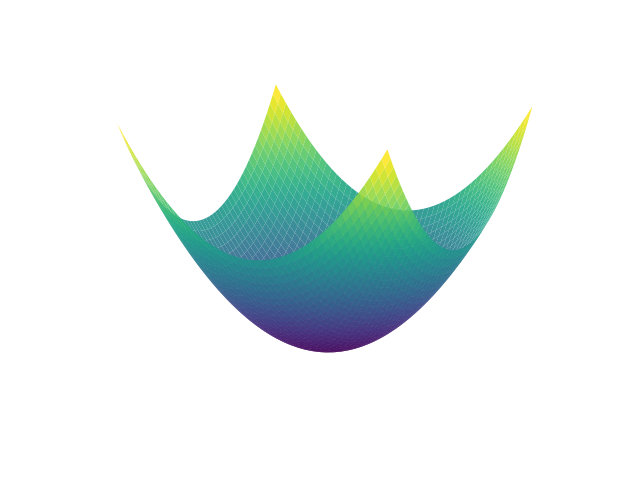
\includegraphics[scale=\myscale,scale=0.35]{figures/gradient-surface-1b}\\
		
		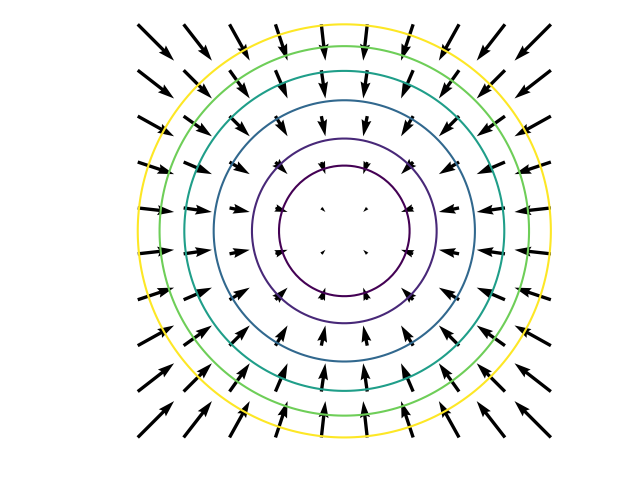
\includegraphics[scale=\myscale,scale=0.35]{figures/gradient-surface-5a}
		
		\quad\textbf{Cas d'un minimum}
	\end{minipage}
	\begin{minipage}{0.30\textwidth}
		\center
		
		\ \ 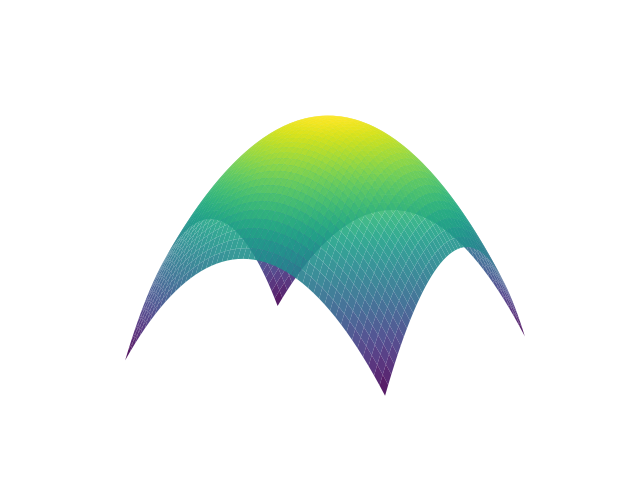
\includegraphics[scale=\myscale,scale=0.35]{figures/gradient-surface-2}\\
		
		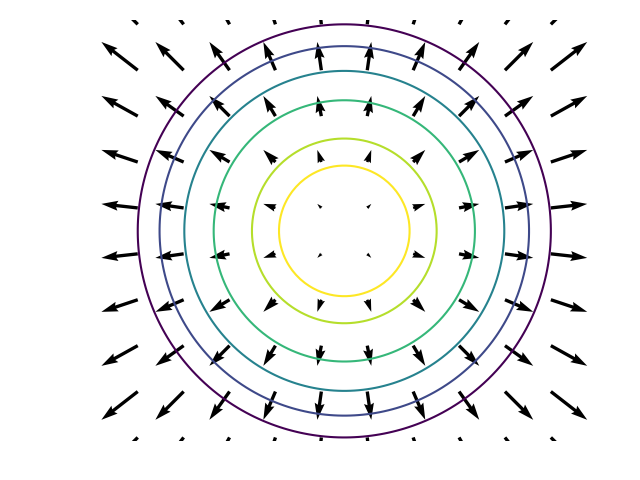
\includegraphics[scale=\myscale,scale=0.35]{figures/gradient-surface-5b}
		
		\quad\textbf{Cas d'un maximum}
	\end{minipage}
	\begin{minipage}{0.30\textwidth}
		\center
		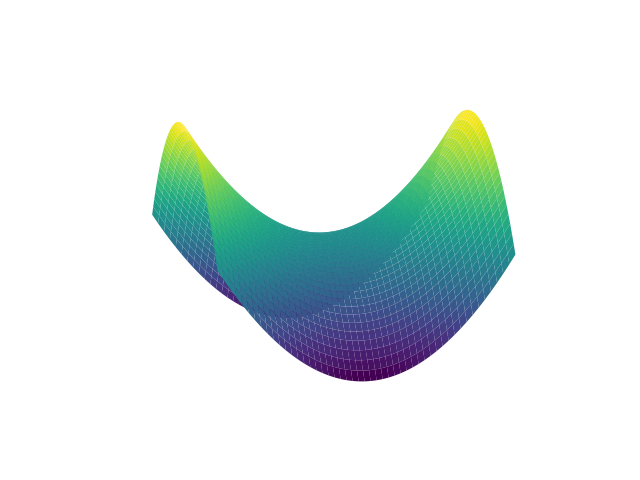
\includegraphics[scale=\myscale,scale=0.35]{figures/gradient-surface-3c}\\
		
		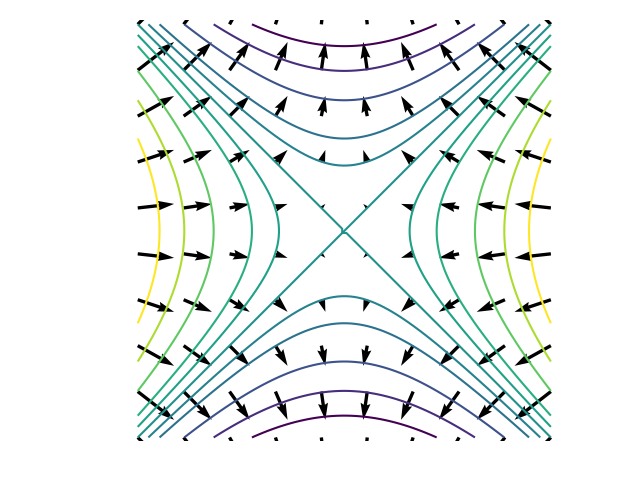
\includegraphics[scale=\myscale,scale=0.35]{figures/gradient-surface-5c}
		
		\quad\textbf{Cas d'un point-selle}
	\end{minipage}
\end{center}

%%%%%%%%%%%%%%%%%%%%%%%%%%%%%%%%%%%%%%%%%%%%%%%%%%%%%%%%%%%%%%%%%%%%%
%\section{Différentiation automatique}
%
%\index{différentiation automatique}
%
%Dans le chapitre \og{}Dérivée\fg{}, nous avons vu comment calculer la dérivée d'une fonction composée à l'aide de son graphe de calcul. Nous allons faire de même pour les dérivées partielles des fonctions de plusieurs variables afin de calculer le gradient d'une fonction définie par un réseau de neurones.
%
%%--------------------------------------------------------------------
%\subsection{Différentiation automatique}
%
%\textbf{Graphe de calcul.}\index{graphe de calcul}
%Voici le graphe de calcul d'une fonction $f$ de deux variables (schéma de principe à gauche, évaluation en $(x_0,y_0)$ à droite).
%
%\myfigure{0.6}{
%	\tikzinput{fig-diffauto-01}\qquad\qquad\qquad
%	\tikzinput{fig-diffauto-02}
%}
%
%
%\bigskip
%\textbf{Dérivées locales.}
%Voici la règle pour les dérivées locales à rajouter à chaque branche (entre crochets).
%\myfigure{0.6}{
%	\tikzinput{fig-diffauto-03}
%}
%On note $\partial_x f$ comme raccourci de la fonction $\frac{\partial f}{\partial x}$.
%
%
%\bigskip
%\textbf{Dérivées partielles.}
%On obtient chacune des dérivées partielles d'une composition $F$ comme le produit des dérivées locales le long des branches allant de la sortie $F(x,y)$ vers l'entrée $x$ (ou $y$).
%\myfigure{0.8}{
%	\tikzinput{fig-diffauto-04}
%}
%
%
%\bigskip
%\textbf{Formule mathématique.}
%Soit $f : \Rr^2 \to \Rr$ et $g : \Rr \to \Rr$. 
%
%\myfigure{0.6}{
%	\tikzinput{fig-diffauto-05}
%}
%La composition $F = g \circ f : \Rr^2 \to \Rr$ correspond au graphe de calcul dessiné ci-dessous :
%\myfigure{0.6}{
%	\tikzinput{fig-diffauto-06}
%}
%
%On a donc :
%$$F(x,y) = g \circ f (x,y) = g \big( f(x,y) \big).$$
%Les dérivées partielles de $F$ sont données par les formules :
%\mybox{$\displaystyle
%	\begin{array}{c}
%		\displaystyle \frac{\partial F}{\partial x}(x_0,y_0) = \frac{\partial f}{\partial x}(x_0,y_0) \cdot g'\big(f(x_0,y_0)\big)\\[4ex]
%		\displaystyle \frac{\partial F}{\partial y}(x_0,y_0) = \frac{\partial f}{\partial y}(x_0,y_0) \cdot g'\big(f(x_0,y_0)\big)
%	\end{array}
%	$}
%
%La preuve de la formule pour $\frac{\partial F}{\partial x}(x_0,y_0)$ découle directement de la formule de la dérivée d'une composition pour la fonction d'une seule variable $x \mapsto F(x,y_0)$. Il en est de même pour l'autre dérivée partielle.
%Ces formules justifient notre règle de calcul : la dérivée partielle est le produit des dérivées locales le long de chacune des branches.
%
%\myfigure{0.8}{
%	\tikzinput{fig-diffauto-07}
%}
%
%
%\bigskip
%\textbf{Addition et multiplication.}
%
%Dans le cas $f(x,y) = x + y$ et $f(x,y)= x \times y$, on retrouve les dérivées locales déjà utilisées dans le cas d'une seule variable.
%
%\myfigure{0.6}{
%	\tikzinput{fig-diffauto-08}\qquad\qquad\qquad
%	\tikzinput{fig-diffauto-09}
%}
%
%
%
%\bigskip
%\textbf{Exemple.}
%Soit $F(x,y) = \ln(x^2y+\sin y)$. On souhaite calculer $\grad F(3,2)$.
%Nous allons montrer comment calculer $\grad F(x_0,y_0)$ pour $x_0$ et $y_0$ quelconques, puis nous reprendrons les calculs depuis le début dans le cas $(x_0,y_0)=(3,2)$.
%
%\myfigure{0.8}{
%	\tikzinput{fig-diffauto-10}
%}
%\myfigure{0.8}{
%	\tikzinput{fig-diffauto-11}
%}
%
%On obtient les dérivées partielles comme produit des dérivées locales :
%$$\frac{\partial F}{\partial x} (x_0,y_0) = \left[ \frac{1}{z_0} \right] \times [2x_0y_0] = \frac{2x_0y_0}{x_0^2y_0+\sin y_0},$$
%$$\frac{\partial F}{\partial y} (x_0,y_0) = \left[ \frac{1}{z_0} \right] \times [x_0^2 + \cos y_0] = \frac{x_0^2 + \cos y_0}{x_0^2y_0+\sin y_0}.$$
%
%
%
%Dans la pratique, pour les réseaux de neurones, on ne calcule jamais l'expression formelle de $\grad F(x_0,y_0)$ mais seulement des gradients en des valeurs $(x_0,y_0)$ données. On reprend donc à chaque fois les étapes ci-dessus mais uniquement pour des valeurs numériques.
%
%
%
%La première étape est de calculer les valeurs des fonctions (de la gauche vers la droite).
%\myfigure{0.8}{
%	\tikzinput{fig-diffauto-12}
%}
%
%La seconde étape est de calculer toutes les dérivées locales. On utilise les valeurs de l'étape précédente et la connaissance des formules de chacune des dérivées des fonctions élémentaires (ici $\frac{\partial f}{\partial x}$, $\frac{\partial f}{\partial y}$ et $\frac{\dd \ln}{\dd z}$).
%
%\myfigure{0.8}{
%	\tikzinput{fig-diffauto-13}
%}
%
%On calcule le produit des dérivées locales le long des arêtes. 
%\myfigure{0.8}{
%	\tikzinput{fig-diffauto-14}
%}
%
%On obtient les dérivées partielles :
%{\small
%	$$\frac{\partial F}{\partial x} (3,2) = \left[ \frac{1}{18+\sin 2} \right] \times [12] = \frac{12}{18 + \sin 2}
%	\qquad \text{ et } \qquad 
%	\frac{\partial F}{\partial y} (3,2) = \left[ \frac{1}{18+\sin 2} \right] \times [9 + \cos 2] = \frac{9 + \cos 2}{18+\sin 2}.$$
%}
%
%\bigskip
%\textbf{Règle générale.}
%Dans le cas de $n$ entrées $(x_1,\ldots,x_n)$, la règle des dérivées locales se généralise naturellement : on associe à la branche numéro $i$ la dérivée locale $\frac{\partial f}{\partial x_i}$.
%
%\myfigure{0.8}{
%	\tikzinput{fig-diffauto-15}
%}
%
%
%%--------------------------------------------------------------------
%\subsection{Différentiation automatique (suite)}
%
%
%\textbf{Graphe de calcul.}
%Voici le graphe de calcul d'une situation que l'on a déjà rencontrée dans le cas d'une seule variable, mais dont la formule se justifie par les fonctions de deux variables.
%Il s'agit du graphe de calcul de $F(t) = f\big( u(t), v(t) \big)$ où
%$u : \Rr \to \Rr$, $v : \Rr \to \Rr$ et $f : \Rr^2 \to \Rr$. L'objectif est de calculer $F'(t)$.
%
%\myfigure{0.55}{
%	\tikzinput{fig-diffauto-21}\qquad
%	\tikzinput{fig-diffauto-22}
%}
%
%\bigskip
%\textbf{Dérivées locales.}
%On calcule les dérivées locales comme d'habitude.
%\myfigure{0.8}{
%	\tikzinput{fig-diffauto-23}
%}
%
%\bigskip
%\textbf{Dérivée.}
%La dérivée s'obtient en deux étapes :
%\begin{itemize}
%	\item on calcule le produit des dérivées locales le long des chemins partant de chaque arête sortante jusqu'à la sortie,
%	\item puis on calcule la somme de ces produits.
%\end{itemize}
%
%\myfigure{0.9}{
%	\tikzinput{fig-diffauto-24}
%}
%
%\bigskip
%\textbf{Formule mathématique.}
%La situation est cette fois la suivante :
%\myfigure{0.6}{
%	\tikzinput{fig-diffauto-25}
%}
%La formule de dérivation de la composition de
%$$F(t) = f\big( u(t), v(t) \big)$$
%est :
%\mybox{$\displaystyle
%	F'(t_0) = u'(t_0) \frac{\partial f}{\partial x}(u(t_0),v(t_0)) \  + \  v'(t_0) \frac{\partial f}{\partial y}(u(t_0),v(t_0)) 
%	$}
%
%
%\bigskip
%\textbf{Exemple.}
%Soit $F(t) = \sqrt{\exp(t)\sin(t)}$. On souhaite calculer $F'(1)$. On commence par calculer $F'(t_0)$ en général avant de tout reprendre dans la cas $t_0=1$.
%Voici le graphe de calcul :
%\myfigure{0.6}{
%	\tikzinput{fig-diffauto-26}
%}
%Une fois complété avec les dérivées locales cela donne :
%\myfigure{0.8}{
%	\tikzinput{fig-diffauto-27}
%}
%On trouve ainsi :
%$$F'(t_0) = \left[\frac{1}{2\sqrt{z_0}}\right]\cdot[y_0]\cdot[\exp t_0]
%\  + \  \left[\frac{1}{2\sqrt{z_0}}\right]\cdot[x_0]\cdot[\cos t_0]
%$$
%et donc 
%$$F'(t_0) = \frac{\exp t_0 \cdot (\sin t_0 + \cos t_0)}{2\sqrt{\exp t_0 \sin t_0}}.$$
%
%Reprenons tout depuis le début pour calculer $F'(1)$ en oubliant que l'on a déjà trouvé la formule générale :
%\myfigure{0.8}{
%	\tikzinput{fig-diffauto-28}
%}
%On trouve ainsi :
%$$F'(1) = \left[\frac{1}{2\sqrt{e\sin(1)}}\right]\cdot[\sin(1)]\cdot[e]
%\  + \  \left[\frac{1}{2\sqrt{e\sin(1)}}\right]\cdot[e]\cdot[\cos(1)]
%$$
%et donc 
%$$F'(1) = \frac{e (\sin(1)+\cos(1))}{2\sqrt{e\sin(1)}}.$$
%
%
%\bigskip
%\textbf{Règle générale.}
%Dans le cas de $n$ sorties, on somme sur toutes les arêtes sortantes comme dans la situation ci-dessous.
%\myfigure{0.8}{
%	\tikzinput{fig-diffauto-29}
%}
%La fonction est $F(t) = t + (\ln t)^2 + \frac{1}{\sin t}$ et en sommant on trouve bien $F'(t) = 1 + \frac{2\ln t}{t} - \frac{\cos t}{\sin^2 t}$.
%
%
%\bigskip
%\textbf{Un autre exemple.}
%On termine par un exemple plus compliqué : on souhaite calculer la dérivée de 
%$$F(t) = t^2 \cdot \ln t \cdot \ln(\ln t).$$
%Voici le graphe de calcul que l'on utilise (noter qu'avec ce graphe, on ne calcule qu'une seule fois $\ln t$ dont le résultat est réutilisé pour calculer $\ln(\ln t)$).
%
%\myfigure{0.8}{
%	\tikzinput{fig-diffauto-30}
%}
%
%La dérivée s'obtient comme somme sur tous les chemins de la sortie à l'entrée.



\index{gradient}
\index{descente de gradient!classique}

%%%%%%%%%%%%%%%%%%%%%%%%%%%%%%%%%%%%%%%%%%%%%%%%%%%%%%%%%%%%%%%%%%%%%
\section{Descente de gradient classique}
L'objectif de la méthode de descente de gradient est de trouver un minimum d'une fonction de plusieurs variables le plus rapidement possible. L'idée est très simple, on sait que le vecteur opposé au gradient indique une direction vers des plus petites valeurs de la fonction, il suffit donc de suivre d'un pas cette direction et de recommencer. Cependant, afin d'être encore plus rapide, il est possible d'ajouter plusieurs paramètres qui demandent pas mal d'ingénierie pour être bien choisis.

Imaginons une goutte d'eau en haut d'une colline. La goutte d'eau descend en suivant la ligne de plus grande pente et elle s’arrête lorsqu'elle atteint un point bas. C'est exactement ce que fait la descente de gradient : partant d'un point sur une surface, on cherche la pente la plus grande en calculant le gradient et on descend d'un petit pas, on recommence à partir du nouveau point jusqu'à atteindre un minimum local.

\begin{center}
	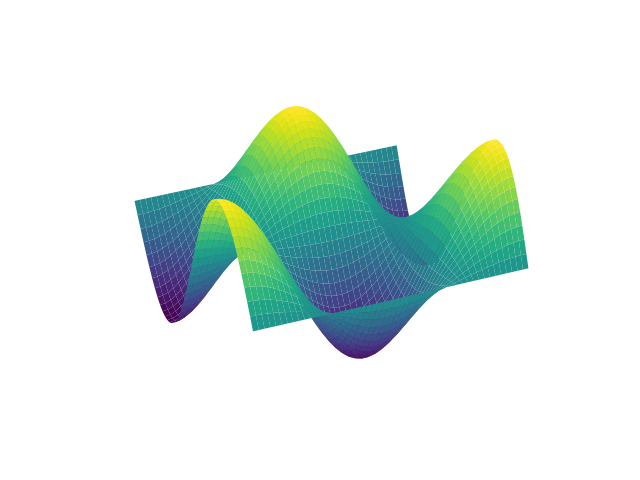
\includegraphics[scale=\myscale,scale=0.6]{figures/descente_intro}
\end{center}


%--------------------------------------------------------------------
\subsection{Où est le minimum ?}

On nous donne une fonction $f$ de deux variables $(a,b)$ et nous cherchons un point
$(a_{\min},b_{\min})$ en lequel $f$ atteint un minimum.
Voici la méthode expliquée par des dessins sur lesquels ont été tracées des lignes de niveau.

\begin{center}
	\begin{minipage}{0.48\textwidth}
		\begin{center}
			{\bf (a) Au départ : rien}
			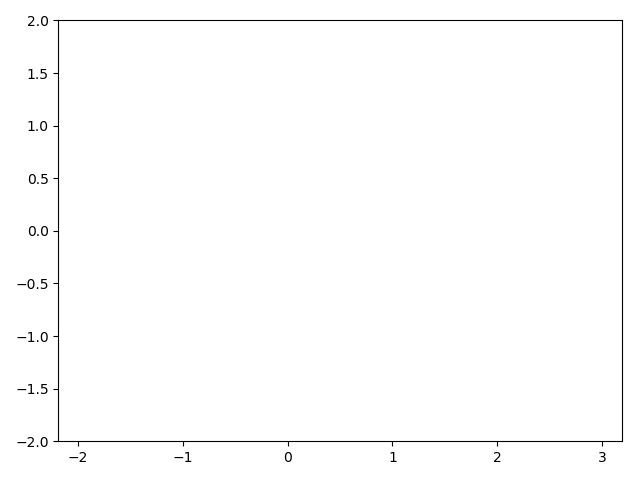
\includegraphics[scale=\myscale,scale=0.5]{figures/descente_intro_01}
		\end{center}
	\end{minipage}
	\begin{minipage}{0.48\textwidth}
		\begin{center}
			{\bf (b) On part d'un point au hasard}
			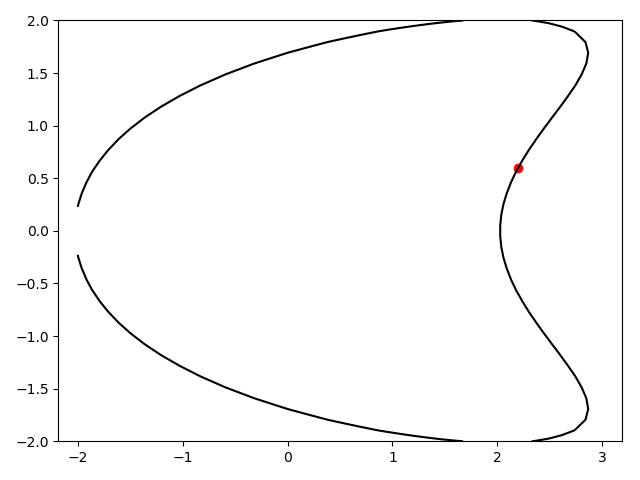
\includegraphics[scale=\myscale,scale=0.5]{figures/descente_intro_02}
		\end{center}
	\end{minipage}
\end{center}

\begin{center}
	\begin{minipage}{0.48\textwidth}
		\begin{center}
			{\bf (c) On suit l'opposé du gradient}
			\includegraphics[scale=\myscale,scale=0.5]{figures/descente_intro_03}
		\end{center}
	\end{minipage}
	\begin{minipage}{0.48\textwidth}
		\begin{center}
			{\bf (d) Depuis le nouveau point, on suit l'opposé du gradient}
			\includegraphics[scale=\myscale,scale=0.5]{figures/descente_intro_04}
		\end{center}
	\end{minipage}
\end{center}

\begin{center}
	\begin{minipage}{0.48\textwidth}
		\begin{center}
			{\bf (e) On répète le processus}
			\includegraphics[scale=\myscale,scale=0.5]{figures/descente_intro_05}
		\end{center}
	\end{minipage}
	\begin{minipage}{0.48\textwidth}
		\begin{center}
			{\bf (f) La suite converge vers le minimum}
			\includegraphics[scale=\myscale,scale=0.5]{figures/descente_intro_06}
		\end{center}
	\end{minipage}
\end{center}

{\bf Figure (a).} Au départ nous n'avons aucune information globale sur $f$. La seule opération que l'on s'autorise c'est calculer $\grad f(a,b)$ en certains points.

{\bf Figure (b).} On choisit un point $(a_0,b_0)$ au hasard. Si on note $c_0 = f(a_0,b_0)$ la valeur de $f$ en ce point, on sait que la ligne de niveau $(f=c_0)$ passe par $(a_0,b_0)$.

{\bf Figure (c).} On calcule en ce point le gradient de $f$. On trace l'opposé du gradient : $-\grad f(a_0,b_0)$. On sait d'une part que la ligne de niveau est orthogonale à ce gradient et surtout que dans la direction de $-\grad f(a_0,b_0)$, les valeurs de $f$ vont diminuer.

\myfigure{0.8}{
	\tikzinput{fig-intro-01}
}

On se dirige alors dans la direction opposée au gradient d'un facteur $\delta$ (par exemple $\delta=0.1$). On arrive à un point noté $(a_1,b_1)$. Par construction, si $\delta$ est assez petit, la valeur $c_1 = f(a_1,b_1)$ est plus petite que $c_0$.

{\bf Figure (d).} On recommence depuis $(a_1,b_1)$. On calcule l'opposé du gradient en $(a_1,b_1)$, on se dirige dans cette nouvelle direction pour obtenir un point $(a_2,b_2)$ où $c_2 = f(a_2,b_2) < c_1$. 

{\bf Figure (e).} On itère le processus pour obtenir une suite de points $(a_k,b_k)$ pour lesquels $f$ prend des valeurs de plus en plus petites. 

{\bf Figure (f).}
On choisit de s'arrêter (selon une condition préalablement établie) et on obtient une valeur approchée $(a_N,b_N)$ du point $(a_{\min},b_{\min})$ en lequel $f$ atteint son minimum. 


\'Evidemment avec la vision globale de la fonction, on se dit qu'on aurait pu choisir un point de départ plus près et que certaines directions choisies ne sont pas les meilleures. Mais souvenez-vous que l'algorithme est \og{}aveugle\fg{}, il ne calcule pas les valeurs de $f$ en les $(a_k,b_k)$ et n'a pas connaissance du comportement de $f$ au voisinage de ces points.



%--------------------------------------------------------------------
\subsection{Exemple en deux variables}

Prenons l'exemple de $f(a,b) = a^2 + 3b^2$ dont le minimum est bien évidemment atteint en $(0,0)$ et appliquons la méthode du gradient.

Nous aurons besoin de calculer la valeur du gradient en certains points par la formule :
$$\grad f(a,b) = \left(\frac{\partial f}{\partial a}(a,b),\frac{\partial f}{\partial b}(a,b)\right) = (2a,6b).$$

Tout d'abord, on part d'un point $(a_0,b_0) = (2,1)$ par exemple.
Même si nous n'en avons pas besoin pour notre construction, on a $f(a_0,b_0) = 7$.
On calcule $\grad f(a_0,b_0) = (4,6)$. On fixe le facteur $\delta = 0.2$. On se déplace dans la direction opposée à ce gradient :
$$(a_1,b_1) = (a_0,b_0) - \delta \grad f(a_0,b_0) = (2,1)-0.2(4,6) = (2,1)-(0.8,1.2) = (1.2, -0.2).$$
On note que $f(a_1,b_1) = 1.56$ est bien plus petit que $f(a_0,b_0)$.
On recommence ensuite depuis $(a_1,b_1)$.
En quelques étapes les valeurs de $f$ tendent vers la valeur minimale et, dans notre cas, la suite converge vers $(0,0)$ (les valeurs sont approchées).

$$
\begin{array}{c|c|c|c}
	k & (a_k,b_k) & \grad f(a_k,b_k) & f(a_k,b_k) \\ \hline
	0 & (2, 1) & (4, 6) & 7 \\
	1 & (1.2, -0.2) & (2.4, -1.20) & 1.56 \\
	2 & (0.72, 0.04) & (1.44, 0.24) & 0.523 \\
	3 & (0.432, -0.008) & (0.864, -0.048) & 0.186 \\
	4 & (0.2592, 0.0016) & (0.5184, 0.0096) & 0.067 \\
	5 & (0.15552, -0.00032) & (0.31104, -0.00192) & 0.024 \\
	\cdots & & & \\
	10 & (0.012, 1.02 \cdot 10^{-7}) & (0.024, 6.14\cdot 10^{-7}) & 0.00014 \\
	\cdots &  & & \\
	20 & (7.31\cdot 10^{-5}, 1.04 \cdot 10^{-14}) & (1.46 \cdot 10^{-4}, 6.29 \cdot 10 ^{-14}) & 5.34 \cdot 10^{-9} \\
\end{array}
$$

\bigskip

Voici les graphiques des premières itérations :
\begin{center}
	\begin{minipage}{0.32\textwidth}
		\begin{center}
			{\bf Point initial}
			\includegraphics[scale=\myscale,scale=0.33]{figures/descente_deux_var_01}
		\end{center}
	\end{minipage}
	\begin{minipage}{0.32\textwidth}
		\begin{center}
			{\bf Une itération}
			\includegraphics[scale=\myscale,scale=0.33]{figures/descente_deux_var_02}
		\end{center}
	\end{minipage}
	\begin{minipage}{0.32\textwidth}
		\begin{center}
			{\bf Deux itérations}
			\includegraphics[scale=\myscale,scale=0.33]{figures/descente_deux_var_03}
		\end{center}
	\end{minipage}
\end{center}

\begin{center}
	\begin{minipage}{0.32\textwidth}
		\begin{center}
			{\bf Trois itérations}
			\includegraphics[scale=\myscale,scale=0.33]{figures/descente_deux_var_04}
		\end{center}
	\end{minipage}
	\begin{minipage}{0.32\textwidth}
		\begin{center}
			{\bf Plus d'itérations}
			\includegraphics[scale=\myscale,scale=0.33]{figures/descente_deux_var_05}
		\end{center}
	\end{minipage}
	
\end{center}

Que se passe-t-il si l'on part d'un autre point ?
Partons cette fois de $(a_0,b_0) = (-1,-1)$ et fixons le pas à $\delta = 0.1$. 
Alors $(a_1,b_1)= (-0.8,-0.4)$, $(a_2,b_2) = (-0.64,-0.16)$\ldots{} 
La suite converge également vers $(0,0)$.
\begin{center}
	\begin{minipage}{0.45\textwidth}
		\begin{center}
			{\bf Partant de $(-1,-1)$ avec $\delta=0.1$}
			\includegraphics[scale=\myscale,scale=0.4]{figures/descente_deux_var_06}
		\end{center}
	\end{minipage}
\end{center}


%--------------------------------------------------------------------
\subsection{Exemples en une variable}

La descente de gradient fonctionne aussi très bien pour les fonctions d'une seule variable et sa visualisation est instructive.

\begin{exemple}
	Considérons la fonction $f : \Rr \to \Rr$ définie par 
	$$f(a) = a^2+1.$$
	Il s'agit de trouver la valeur en laquelle $f$ atteint son minimum, c'est clairement $a_{\min}=0$ pour lequel $f(a_{\min})=1$. Retrouvons ceci par la descente de gradient.
	
	Partant d'une valeur $a_0$ quelconque, la formule de récurrence est :
	$$a_{k+1} = a_k - \delta \grad f(a)$$
	où $\delta$ est le pas, choisi assez petit, et $\grad f(a) = f'(a) = 2a$.
	Autrement dit :
	$$a_{k+1} = a_k - 2 \delta a_k.$$
	
	Voici le tableau des valeurs pour un pas $\delta=0.2$ et une valeur initiale $a_0=2$.
	
	$$
	\begin{array}{c|c|c|c}
		k & a_k & f'(a_k) = \grad f(a_k) & f(a_k) \\ \hline
		0 & 2 & 4 & 5 \\
		1 & 1.2 & 2.4 & 2.44 \\
		2 & 0.72 & 1.44 & 1.5184 \\
		3 & 0.43 & 0.86 & 1.1866 \\
		4 & 0.25 & 0.5184 & 1.0671 \\
		5 & 0.15 & 0.31 & 1.0241 \\
		6 & 0.093 & 0.186 & 1.0087 \\
		7 & 0.055 & 0.111 & 1.0031 \\
		8 & 0.033 & 0.067 & 1.0011 \\
		9 & 0.020 & 0.040 & 1.0004 \\
		10 & 0.012 & 0.024 & 1.0001 \\
	\end{array}
	$$
	
	Voici la version graphique de ces $10$ premières itérations (figure de gauche).
	Si l'on change le point initial, ($a_0=-1.5$ sur la figure de droite) alors la suite $(a_k)$ converge vers la même valeur $a_{\min}=0$.
	
	\begin{center}
		\begin{minipage}{0.48\textwidth}
			\begin{center}
				$\delta=0.2$ \quad $a_0=2$
				\includegraphics[scale=\myscale,scale=0.5]{figures/descente_une_var_01}
			\end{center}
		\end{minipage}
		\begin{minipage}{0.48\textwidth}
			\begin{center}
				$\delta=0.2$ \quad $a_0=-1.5$
				\includegraphics[scale=\myscale,scale=0.5]{figures/descente_une_var_02}
			\end{center}
		\end{minipage}
	\end{center}
	
	Il faut bien comprendre ce graphique : la suite des points $(a_k)$ \couleurnb{(points rouges) }{}se lit sur l'axe des abscisses. Les vecteurs \couleurnb{(orange) }{}montrent les itérations.
	Il est plus facile de comprendre l'algorithme sur le graphe de $f$\couleurnb{ (en bleu)}{}. Sur ce graphe, on reporte les points $(a_k,f(a_k))$\couleurnb{ (en rouge)}{}, ce qui permet de bien comprendre que les valeurs $f(a_k)$ décroissent rapidement. On note aussi que le gradient (ici $f'(a_k)$) diminue à l'approche du minimum, ce qui se traduit par des vecteurs (c'est-à-dire l'écart entre deux points successifs) de plus en plus petits. 
	
\end{exemple}

Justifions l'algorithme et l'intervention du gradient dans le cas d'une variable.
Si la fonction est croissante sur un intervalle, $f'(a)>0$ pour tout $a$ dans cet intervalle et la formule
$$a_{k+1} = a_k - \delta f'(a_k) \quad \text{ donne } \quad a_{k+1}<a_k.$$
Ainsi $f(a_{k+1}) < f(a_k)$ et l'ordonnée du point $(a_{k+1},f(a_{k+1}))$ est donc inférieure à celle du point $(a_k,f(a_k))$.
Par contre, si $f$ est décroissante alors $f'(a)<0$ et
$$a_{k+1} = a_k - \delta f'(a_k) \quad \text{ donne } \quad a_{k+1}>a_k,$$
ce qui implique de nouveau $f(a_{k+1}) < f(a_k)$ (car $f$ est décroissante).

Dans tous les cas, l'ordonnée du point $(a_{k+1},f(a_{k+1}))$ est inférieure à celle du point $(a_k,f(a_k))$.

\myfigure{1}{
	\tikzinput{fig_descente-02}
}

\begin{exemple}{}{}
	Le choix du paramètre $\delta$ est important.
	Reprenons la fonction $f$ définie par $f(x) = x^2+1$ et testons différentes \og{}mauvaises\fg{} valeurs du pas $\delta$ (avec toujours $a_0=2$).
	
	\begin{center}
		\begin{minipage}{0.32\textwidth}
			\begin{center}
				$\delta=0.9$
				\includegraphics[scale=\myscale,scale=0.3]{figures/descente_une_var_03}
			\end{center}
		\end{minipage}
		\begin{minipage}{0.32\textwidth}
			\begin{center}
				$\delta=1.1$
				\includegraphics[scale=\myscale,scale=0.3]{figures/descente_une_var_04}
			\end{center}
		\end{minipage}
		\begin{minipage}{0.32\textwidth}
			\begin{center}
				$\delta=0.05$
				\includegraphics[scale=\myscale,scale=0.3]{figures/descente_une_var_05}
			\end{center}
		\end{minipage}
	\end{center}
	
	\begin{itemize}
		\item Pour $\delta = 0.9$, la suite $(a_k)$ tend bien vers $a_{\min} = 0$. Les ordonnées sont bien décroissantes mais comme $\delta$ est trop grand, la suite des points oscille de part et d'autre du minimum.
		
		\item Pour $\delta = 1.1$, la suite $(a_k)$ diverge. Les ordonnées augmentent, la suite des points oscille et s'échappe. Cette valeur de $\delta$ ne donne pas de convergence vers un minimum.
		
		\item Pour $\delta = 0.05$, la suite $(a_k)$ tend bien vers $a_{\min}$ mais, comme $\delta$ est trop petit, il faudrait beaucoup d'itérations pour arriver à une approximation raisonnable.
		
	\end{itemize}
\end{exemple}

\begin{exemple}{}{}
	Le choix du point de départ est également important surtout lorsqu'il existe plusieurs minimums locaux.
	Soit la fonction $f$ définie par :
	$$f(a) = a^4 -5a^2 + a + 10.$$
	Cette fonction admet deux minimums locaux.
	La suite $(a_k)$ de la descente de gradient converge vers l'un de ces deux minimums selon le choix du point initial $a_0$ (ici $\delta=0.02$).
	
	\begin{center}
		\begin{minipage}{0.48\textwidth}
			\begin{center}
				$a_0=-2$
				\includegraphics[scale=\myscale,scale=0.5]{figures/descente_une_var_06}
			\end{center}
		\end{minipage}
		\begin{minipage}{0.48\textwidth}
			\begin{center}
				$a_0=-0.5$
				\includegraphics[scale=\myscale,scale=0.5]{figures/descente_une_var_07}
			\end{center}
		\end{minipage}
		
		\bigskip
		
		\begin{minipage}{0.48\textwidth}
			\begin{center}
				$a_0=0.5$
				\includegraphics[scale=\myscale,scale=0.5]{figures/descente_une_var_08}
			\end{center}
		\end{minipage}
		\begin{minipage}{0.48\textwidth}
			\begin{center}
				$a_0=2$
				\includegraphics[scale=\myscale,scale=0.5]{figures/descente_une_var_09}
			\end{center}
		\end{minipage}
	\end{center}
\end{exemple}


\begin{exemple}{}{}
	Les points-selles posent également problème.
	
	La fonction $f$ définie par 
	$$f(a) = a^4-2a^3+4$$
	a pour dérivée $f'(a) = 4a^3-6a^2$ qui s'annule en $a=0$ qui est l'abscisse d'un point-selle (ni un  minimum ni un maximum, en fait la fonction est strictement décroissante autour de $a=0$). La dérivée s'annule aussi en $a=\frac32$ où est atteint le minimum global.
	
	Voici les $100$ premières itérations pour la descente de gradient en partant de $a_0=-1$ (avec $\delta = 0.05$) : la suite $a_k$ converge vers $0$ qui n'est pas le minimum recherché.
	
	\begin{center}
		\includegraphics[scale=\myscale,scale=0.5]{figures/descente_une_var_10}
	\end{center}
\end{exemple}

%--------------------------------------------------------------------
\subsection{Algorithme du gradient}

Formalisons un peu les choses pour mettre en évidence l'idée générale et les problèmes techniques qui surviennent.

\textbf{Algorithme de la descente de gradient.}


Soit une fonction $f : \Rr^n \to \Rr$, $P \mapsto f(P)$ de plusieurs variables, avec $P = (a_1,\ldots,a_n)$, dont on sait calculer le gradient $\grad f (P)$.

\textbf{Données.}
\begin{itemize}
	\item Un point initial $P_0 \in \Rr^n$.
	\item Un niveau d'erreur $\epsilon>0$. 
\end{itemize}

\textbf{Itération.}
On calcule une suite de points $P_1,P_2,\ldots \in \Rr^n$ par récurrence de la façon suivante. Supposons que l'on ait déjà obtenu le point $P_k$ :
\begin{itemize}
	\item on calcule $\grad f(P_k)$,
	\item on choisit un pas $\delta_k$ et on calcule
	$$P_{k+1} = P_k - \delta_k \grad f (P_k).$$
\end{itemize}  

\myfigure{1}{
	\tikzinput{fig_descente-01}
}


\textbf{Arrêt.}
On s'arrête lorsque $\|\grad f(P_k) \| \le \epsilon$.


\bigskip


	\begin{itemize}
		\item \'Evidemment, plus on choisit le point initial $P_0$ proche d'un minimum local, plus l'algorithme va aboutir rapidement. Mais comme on ne sait pas où est ce minimum local (c'est ce que l'on cherche), le plus simple est de choisir un $P_0$ au hasard.
		
		\item Le choix du pas $\delta_k$ est crucial. On sait que l'on peut choisir $\delta_k$ assez petit de façon à avoir $f(P_{k+1}) \le f(P_k)$ car dans la direction de $-\grad f(P_k)$ la fonction $f$ décroît.
		
		\myfigure{1}{
			\tikzinput{fig_descente-03}
		}
		
		On peut fixer à l'avance un pas $\delta$ commun à toutes les itérations, par exemple $\delta = 0.01$. On pourrait également tester à chaque itération plusieurs valeurs de $\delta$ par balayage ($\delta = 0.001$, puis $\delta=0.002$\ldots) et choisir pour $\delta_k$ celui en lequel $f$ prend la plus petite valeur.
		
		\item Le critère d'arrêt assure qu'en $P_k$ le gradient est très petit. Cela ne garantit pas que ce point soit proche d'un minimum local (et encore moins d'un minimum global). Souvenez-vous : en un minimum local le gradient est nul, mais ce n'est pas parce que le gradient est nul que l'on a atteint un minimum local, cela pourrait être un point-selle voire un maximum local.
		
		Dans la pratique, on ne définira pas de seuil d'erreur $\epsilon$, mais un nombre d'itérations fixé à l'avance.
		
		\item Il est important de calculer $\grad f(a_1,\ldots,a_n)$ rapidement. On pourrait bien sûr calculer une approximation de chacune des dérivées partielles $\frac{\partial f}{\partial a_i}(a_1,\ldots,a_n)$ comme un limite. Mais pour gagner en temps et en précision, on préfère que ce calcul soit fait à l'aide de son expression exacte. 
		
	\end{itemize}
%%%%%%%%%%%%%%%%%%%%%%%%%%%%%%%%%%%%%%%%%%%%%%%%%%%%%%%%%%%%%%%%%%%%%
\section{Optimisation : théorie}
\subsection{Formule de Taylor à l'ordre 2}

Soit $f : \Rr \to \Rr$ une fonction d'une variable de classe $\mathcal{C}^2$. 
\begin{theoreme}{Formule de Taylor à l'ordre $2$}{} 
Pour tout $x_0 \in \Rr$, on a
\mybox{$f(x_0 + h) = f(x_0) + hf'(x_0) + \frac{h^2}{2} f''(x_0) + h^2 \epsilon(h)$}
où $\epsilon(h) \to 0$ lorsque $h\to0$.
\end{theoreme}

Le développement limité à l'ordre $1$, $f(x_0 + h) \simeq f(x_0) + hf'(x_0)$, correspond à l'approximation du graphe de $f$ par sa tangente en $x_0$ (figure de gauche ci-dessous).
Le développement limité à l'ordre $2$, $f(x_0 + h) \simeq f(x_0) + hf'(x_0) + \frac{h^2}{2} f''(x_0)$, correspond à une approximation par une parabole (figure de droite).


\myfigure{0.7}{
    \tikzinput{fig-extrem-04a}\qquad \qquad 
    \tikzinput{fig-extrem-04b}    
}


Choisissons pour $x_0$ une valeur telle que $f'(x_0)=0$ et $f''(x_0)\neq 0$. 
Alors, pour $h$ assez petit, le terme $ \frac{h^2}{2} f''(x_0) + h^2 \epsilon (h)$ est du même signe que $f''(x_0)$. Si par exemple $f''(x_0)>0$, on en déduit que $f(x_0 + h) \ge f(x_0)$ (pour $h$ proche de $0$) et donc que $f$ admet un minimum local en $x_0$.
Ci-dessous, on va en déduire une caractérisation des minimums et maximums.

%----------------------------------------------------
\subsection{Caractérisation des minimums et maximums}

La recherche pratique des extremums locaux pour une fonction d'une variable se passe donc ainsi :
\begin{enumerate}
    \item On recherche les points critiques donnés par l'équation $f'(x) = 0$.
    \item Pour chaque point critique $x_0$, on calcule la dérivée seconde :
    \begin{itemize}
        \item si $f''(x_0) > 0$, alors $f$ admet un minimum local en $x_0$,   
        \item si $f''(x_0) < 0$, alors $f$ admet un maximum local en $x_0$,
        \item si $f''(x_0) = 0$, alors  il faut approfondir l'étude.
    \end{itemize}    
\end{enumerate}
    
Lorsque $f : [a,b] \to \Rr$ est définie sur un intervalle compact, il faudra en plus étudier le comportement de $f$ en $a$ et en $b$ (c'est-à-dire au bord du domaine de définition). Comme l'ensemble de départ est compact, on a la garantie de l'existence d'extremums globaux.
    

%%%%%%%%%%%%%%%%%%%%%%%%%%%%%%%%%%%%%%%%%%%%%%%%%%%%%
\section{Dérivées partielles d'ordre 2}

%----------------------------------------------------
\subsection{Dérivées partielles d'ordre 2}

Soit $f : \Rr^2 \to \Rr$ une application différentiable.
Les deux dérivées partielles $\frac{\partial f}{\partial x}$
et $\frac{\partial f}{\partial y}$ sont aussi des fonctions de $\Rr^2$ dans $\Rr$ ; 
supposons que ce soient aussi des applications différentiables.
Alors on peut calculer les dérivées partielles de $\frac{\partial f}{\partial x}$ :
$$\frac{\partial}{\partial x}\left(\frac{\partial f}{\partial x}\right)
\qquad \text{ et } \qquad 
\frac{\partial}{\partial y}\left(\frac{\partial f}{\partial x}\right).$$
On peut aussi calculer les dérivées partielles de $\frac{\partial f}{\partial y}$ :
$$\frac{\partial}{\partial x}\left(\frac{\partial f}{\partial y}\right)
\qquad \text{ et } \qquad 
\frac{\partial}{\partial y}\left(\frac{\partial f}{\partial y}\right).$$

On note ces dérivées partielles :
$$\frac{\partial ^2 f}{\partial x^2}
\qquad
\frac{\partial ^2 f}{\partial y\partial x}
\qquad
\frac{\partial ^2 f}{\partial x\partial y}
\qquad
\frac{\partial ^2 f}{\partial y^2}
$$
Ce sont des fonctions de $\Rr^2$ dans $\Rr$.


Plus généralement, pour $f : \Rr^n \to \Rr$, on note $\frac{\partial f}{\partial x_i} : \Rr^n \to \Rr$ les dérivées partielles d'ordre $1$ ($1 \le i \le n$)
et $\frac{\partial ^2f}{\partial x_j\partial x_i}$ les dérivées partielles d'ordre $2$ ($1 \le i,j \le n$).


%----------------------------------------------------
\subsection{Théorème de Schwarz}


Pour $f : \Rr^2 \to \Rr$, il y a quatre dérivées partielles secondes à calculer, mais en général deux d'entre elles sont égales.

\begin{exemple}{}{}
Soit $f : U \to \Rr$ définie par $f(x,y) = x^2\cos(y) + \ln(x-y^2)$ sur $U = \big\{ (x,y) \in \Rr^2 \mid x-y^2>0 \big\}$.
Alors :
$$\frac{\partial f}{\partial x}(x,y) = 2x\cos(y) + \frac{1}{x-y^2}
\qquad\qquad
\frac{\partial f}{\partial y}(x,y) = -x^2\sin(y) - \frac{2y}{x-y^2}$$

On peut maintenant dériver une nouvelle fois pour obtenir les dérivées partielles d'ordre $2$ :
$$\frac{\partial ^2 f}{\partial x^2}(x,y) 
= \frac{\partial}{\partial x}\left(\frac{\partial f}{\partial x}(x,y)\right)
= \frac{\partial}{\partial x}\left(2x\cos(y) + \frac{1}{x-y^2}\right)
= 2\cos(y) - \frac{1}{(x-y^2)^2}$$

$$\frac{\partial ^2 f}{\partial y\partial x}(x,y) 
= \frac{\partial}{\partial y}\left(\frac{\partial f}{\partial x}(x,y)\right)
= \frac{\partial}{\partial y}\left(2x\cos(y) + \frac{1}{x-y^2}\right)
= \boxed{-2x\sin(y) + \frac{2y}{(x-y^2)^2}}$$

$$\frac{\partial ^2 f}{\partial x\partial y}(x,y) 
= \frac{\partial}{\partial x}\left(\frac{\partial f}{\partial y}(x,y)\right)
= \frac{\partial}{\partial x}\left(-x^2\sin(y) - \frac{2y}{x-y^2}\right)
= \boxed{-2x\sin(y) + \frac{2y}{(x-y^2)^2}}$$

$$\frac{\partial ^2 f}{\partial y^2}(x,y) 
= \frac{\partial}{\partial y}\left(\frac{\partial f}{\partial y}(x,y)\right)
= \frac{\partial}{\partial y}\left(-x^2\sin(y) - \frac{2y}{x-y^2}\right)
= -x^2\cos(y) - \frac{2x+2y^2}{(x-y^2)^2}$$


\end{exemple}

On note sur l'exemple précédent que $\frac{\partial ^2 f}{\partial y\partial x}(x,y) = \frac{\partial ^2 f}{\partial x\partial y}(x,y)$. C'est un phénomène général que l'on va détailler.


\begin{definition}{}{}
    Une fonction $f : \Rr^n \to \Rr$ est de \trouer{classe $\mathcal{C}^2$} si $f$ est de classe $\mathcal{C}^1$ (c'est-à-dire ses dérivées partielles existent et sont continues) et si ses dérivées partielles sont aussi de classe $\mathcal{C}^1$.
\end{definition}

Le théorème de Schwarz dit que le résultat ne dépend pas de l'ordre dans lequel on effectue les dérivations.
\begin{theoreme}{Théorème de Schwarz}{}
Soit $f:U\subset \Rr^n\to \Rr$ une fonction de classe $\mathcal{C}^2$. 
Pour tous $i,j  \in \{1,\dots ,n\}$, on a :
    \mybox{$\displaystyle \frac{\partial}{\partial x_i}\left(\frac{\partial f}{\partial x_j}\right)=\frac{\partial}{\partial x_j}\left(\frac{\partial f}{\partial x_i}\right)$}
\end{theoreme}

Ainsi, pour $f : \Rr^2 \to \Rr$ de classe $\mathcal{C}^2$, on a :
\mybox{$\displaystyle \frac{\partial ^2 f}{\partial y\partial x}(x,y) = \frac{\partial ^2 f}{\partial x\partial y}(x,y)$}

Pour $f : \Rr^3 \to \Rr$ de classe $\mathcal{C}^2$, il y a $9$ dérivées partielles d'ordre $2$, mais seulement $6$ calculs à faire :
 $$\frac{\partial ^2 f}{\partial x^2}
 \qquad
 \frac{\partial ^2 f}{\partial y^2}
 \qquad
 \frac{\partial ^2 f}{\partial z^2}  
 \qquad 
 \frac{\partial ^2 f}{\partial y\partial x}= \frac{\partial ^2 f}{\partial x\partial y}
 \qquad
 \frac{\partial ^2 f}{\partial z\partial x}= \frac{\partial ^2 f}{\partial x\partial z}
 \qquad
 \frac{\partial ^2 f}{\partial z\partial y}= \frac{\partial ^2 f}{\partial y\partial z} 
 $$


Le contre-exemple suivant, qui peut être omis lors d'une première lecture, prouve qu'il est nécessaire d'avoir une fonction de classe $\mathcal{C}^2$. Si cette hypothèse manque alors les dérivées partielles croisées peuvent ne pas être égales.

\begin{exemple}
Soit $f: \Rr^2 \to \Rr$ la fonction définie par
$$f(x,y)=\frac{xy^3}{x^2+y^2}\;\mbox{ si }(x,y)\neq (0,0)\quad \mbox{et}\quad f(0,0)= 0.$$
On vérifie que $f$ est de classe $\mathcal{C}^1$ sur $\Rr^2$ et que
$$\frac{\partial f}{\partial x}(x,y)=\left\{\begin{array}{cl}\displaystyle \frac{y^5-x^2y^3}{(x^2+y^2)^2}&\mbox{si }(x,y)\neq (0,0)\\ 0&\mbox{si }(x,y)=(0,0)
\end{array}\right.$$
et 
$$\frac{\partial f}{\partial y}(x,y)=\left\{\begin{array}{cl}\displaystyle \frac{3x^3y^2+xy^4}{(x^2+y^2)^2}&\mbox{si }(x,y)\neq (0,0)\\ 0&\mbox{si }(x,y)=(0,0).\end{array}\right.$$
Le taux d'accroissement
$$\frac{\frac{\partial f}{\partial x}(0,y)-\frac{\partial f}{\partial x}(0,0)}{y-0}=1\underset{y\to 0\; \; \; }{\longrightarrow 1}$$
ce qui montre que $\displaystyle \frac{\partial ^2f}{\partial y\partial x}(0,0)=1$.
De même, le taux d'accroissement
$$\frac{\frac{\partial f}{\partial y}(x,0)-\frac{\partial f}{\partial y}(0,0)}{x-0}=0\underset{x\to 0\; \; \; }{\longrightarrow 0}$$
ce qui montre que $\displaystyle \frac{\partial ^2f}{\partial x\partial y}(0,0)=0$. 
Les dérivées partielles croisées ne sont pas égales en $(0,0)$.
On en déduit que l'une (au moins) des dérivées partielles secondes $\displaystyle \frac{\partial ^2f}{\partial x\partial y}$ ou $\displaystyle \frac{\partial ^2f}{\partial y\partial x}$ n'est pas continue en $(0,0)$. Autrement dit, la fonction $f$ n'est pas de classe $\mathcal{C}^2$ en $(0,0)$ et le théorème de Schwarz ne s'applique pas.
\end{exemple}


%----------------------------------------------------
\subsection{Hessienne}

La matrice jacobienne est la matrice des dérivées partielles.
La matrice hessienne est la matrice des dérivées partielles d'ordre $2$.

Soit $f : \Rr^n \to \Rr$ une fonction de $n$ variables.
La \trouer{matrice hessienne} de $f$ en $x=(x_1,\ldots,x_n)$ est la matrice $n \times n$ :
\mybox{$\displaystyle H_f(x) = \left( \frac{\partial ^2f}{\partial x_i\partial x_j}(x) \right)_{1 \le i,j \le n}$}
Pour une fonction de classe $\mathcal{C}^2$, d'après le théorème de Schwarz, c'est une \evidence{matrice symétrique}.


Dans le cas d'une fonction de deux variables :
\mybox{$\displaystyle 
H_f(x,y)
 = 
\begin{pmatrix}
\frac{\partial ^2f}{\partial x^2}(x,y) & \frac{\partial ^2f}{\partial x\partial y}(x,y) \\
\frac{\partial ^2f}{\partial y\partial x}(x,y) & \frac{\partial ^2f}{\partial y^2}(x,y) \\
\end{pmatrix}$}
% = 
%\begin{pmatrix}
%r(x,y) & s(x,y) \\
%s(x,y) & t(x,y) \\
%\end{pmatrix}
%$$

\bigskip

Pour trois variables, la matrice hessienne (à évaluer en $(x,y,z)$) vaut :
$$H_f=
\begin{pmatrix}
\frac{\partial^2f}{\partial x^2}&\frac{\partial^2f}{\partial x\partial y}&\frac{\partial^2f}{\partial x\partial z}\\  \frac{\partial^2f}{\partial y\partial x}&\frac{\partial^2f}{\partial y^2}&\frac{\partial^2f}{\partial y\partial z}\\  \frac{\partial^2f}{\partial z\partial x}&\frac{\partial^2f}{\partial z\partial y}&\frac{\partial^2f}{\partial z^2}\\
\end{pmatrix}.$$

\begin{exemple}
Calculons la matrice hessienne de $f(x,y) = xy^2 + x^4 - y^4$.

On calcule d'abord 
$$\frac{\partial f}{\partial x}(x,y) = 4x^3 + y^2
\qquad\qquad
\frac{\partial f}{\partial y}(x,y) = 2xy - 4y^3.$$

On a donc 
$$H_f(x,y)
= \begin{pmatrix}
    \frac{\partial ^2f}{\partial x^2}(x,y) & \frac{\partial ^2f}{\partial x\partial y}(x,y) \\
    \frac{\partial ^2f}{\partial y\partial x}(x,y) & \frac{\partial ^2f}{\partial y^2}(x,y) \\
\end{pmatrix}
= 
\begin{pmatrix}
12x^2 & 2y \\
2y      & 2x - 12y^2 \\
\end{pmatrix}.$$
\end{exemple}


%----------------------------------------------------
\paragraph{Exercices}
    \begin{enumerate}
        \item Soit $f(x,y) = x^3+5x^2y-y^2$. Calculer les dérivées partielles d'ordre $1$ de $f$. Calculer les dérivées partielles d'ordre $2$ de $f$. Vérifier la validité du théorème de Schwarz. Calculer la matrice hessienne de $f$. Calculer les dérivées partielles d'ordre $3$ de $f$.
        
        \item Soit $f(x,y) = xe^{x^2-y^2}$. Calculer les dérivées partielles d'ordre $1$ et d'ordre $2$ de $f$. Calculer la matrice hessienne de $f$.
        
        \item Soit $f(x,y,z) = xy^2 \ln(z)$. Déterminer l'ensemble de définition de $f$. Calculer les dérivées partielles d'ordre $1$ et d'ordre $2$ ainsi que la matrice hessienne de $f$.                
    \end{enumerate}


%%%%%%%%%%%%%%%%%%%%%%%%%%%%%%%%%%%%%%%%%%%%%%%%%%%%%
\section{Formule de Taylor à l'ordre 2}

%----------------------------------------------------
\subsection{Formule de Taylor à l'ordre 1}

Nous avons déjà vu qu'une façon de dire que $f$ est différentiable est de dire que $f$ admet un \trouer{développement limité à l'ordre $1$}. Pour $f : \Rr^2 \to \Rr$,
au point $(x_0,y_0)$, si $f$ est différentiable alors
$$f(x_0+h,y_0+k)=f(x_0,y_0)+h\frac{\partial f}{\partial x}(x_0,y_0)+k\frac{\partial f}{\partial y}(x_0,y_0)+o\left(\|(h,k)\|\right).$$

Connaissant les valeurs de $f$, $\frac{\partial f}{\partial x}$
et $\frac{\partial f}{\partial y}$ uniquement en $(x_0,y_0)$, on en déduit une approximation de $f$ en tout $(x,y)$ proche de $(x_0,y_0)$.

\medskip

Le but va être d'améliorer cette approximation par un développement limité à l'ordre $2$.

On rappelle la notation \og{}petit o\fg{}.

\textbf{Notation.} Soit $g :\Rr^2\to \Rr$ une fonction définie au voisinage de $(0,0)$. On dit que $g$ est \trouer{négligeable} par rapport à $\|(x,y)\|^n$ au voisinage de $(0,0)$ et on note $g=o\left(\|(x,y)\|^n\right)$ si 
$$\lim_{(x,y)\to(0,0)}\frac{g(x,y)}{\|(x,y)\|^n}=0.$$

\textbf{Interprétation géométrique.}

Le plan tangent (en bleu) au graphe de $f$ au point $(x_0,y_0)$ est le plan qui approche le mieux le graphe de $f$ (en rouge) autour de ce point.
Pour calculer $f(x,y)$ lorsque $(x,y)=(x_0+h,y_0+k)$ est proche de $(x_0,y_0)$, on remplace la valeur exacte $z_{exact} = f(x,y)$ 
par son approximation $z_{approx} = f(x_0,y_0)+h\frac{\partial f}{\partial x}(x_0,y_0)+k\frac{\partial f}{\partial y}(x_0,y_0)$.
Le point $(x,y,z_{exact})$ est un point du graphe de $f$ alors que
$(x,y,z_{approx})$ est un point du plan tangent au graphe de $f$ au point $(x_0,y_0)$. 


 \myfigure{1}{
     \tikzinput{fig-extrem-06}        
 }


%----------------------------------------------------
\subsection{Formule de Taylor à l'ordre 2 (en 2 variables)}

\begin{theoreme}{}{}    
Soit $f:U \to \Rr$ une fonction de classe $\mathcal{C}^2$ sur un ouvert $U\subset \Rr^2$ et soit $(x_0,y_0)\in U$.  Alors :
\mybox{\begin{align*}
f(x_0+h,y_0+k) 
& = f(x_0,y_0)
\ + \  h\frac{\partial f}{\partial x}(x_0,y_0)
+k\frac{\partial f}{\partial y}(x_0,y_0) \\
& \qquad +\frac{1}{2}\left[
h^2\frac{\partial ^2f}{\partial x^2}(x_0,y_0)
+2hk\frac{\partial ^2f}{\partial x\partial y}(x_0,y_0)
+k^2\frac{\partial ^2f}{\partial y^2}(x_0,y_0)
\right] \\ 
& \qquad \qquad +o\left(\|(h,k)\|^2\right)
\end{align*}}
   
\end{theoreme}


\begin{itemize}
    \item On dit aussi que $f$ admet un développement limité d'ordre $2$ au point $(x_0,y_0)$.

    \item Attention à ne pas oublier le facteur $\frac12$ devant les termes de degré $2$, ni le facteur $2$ devant le terme $hk$.
    
    \item On rappelle que si on choisit la norme euclidienne alors $\|(h,k)\|^2 = h^2+k^2$ et que $o\left(\|(h,k)\|^2\right)$ désigne une fonction égale à $\|(h,k)\|^2 \epsilon(h,k)$ avec $\epsilon(h,k) 
    \xrightarrow[(h,k)\to (0,0)]{} 0.$


\end{itemize}



\begin{exemple}{}{}
Étudions $f(x,y) = \exp(xy^2-2)$ autour de $(x_0,y_0) = (2,1)$.
\begin{itemize}
    \item $f(2,1) = 1$.
    
    \item \textbf{DL à l'ordre 1.}
    $$\frac{\partial f}{\partial x}(x,y) = y^2\exp(xy^2-2)
    \quad
    \frac{\partial f}{\partial y}(x,y) = 2xy\exp(xy^2-2)
    \quad\text{ donc }\quad
    \frac{\partial f}{\partial x}(2,1) = 1
    \quad
    \frac{\partial f}{\partial y}(2,1) = 4$$
    Ainsi :
    $$f(2+h,1+k) = 1 + h + 4k + o\left(\|(h,k)\|\right).$$
  
    \item \textbf{DL à l'ordre 2.} 
    
    \begin{align*}
    \frac{\partial ^2f}{\partial x^2}(x,y) &= y^4\exp(xy^2-2) \\
    \frac{\partial ^2f}{\partial x\partial y}(x,y) &= (2y+2xy^3)\exp(xy^2-2)\\
    \frac{\partial ^2f}{\partial y^2}(x,y) &= (2x+4x^2y^2)\exp(xy^2-2)
    \end{align*}
    Donc :
    $$\frac{\partial ^2f}{\partial x^2}(2,1) = 1\qquad 
    \frac{\partial ^2f}{\partial x\partial y}(2,1) = 6 \qquad
    \frac{\partial ^2f}{\partial y^2}(2,1) = 20.$$ 
    Ainsi :
    $$   
    f(2+h,1+k)  \ 
    = \  1 \quad + \quad h + 4k
    \quad +\quad
    \frac12\left(h^2
    +2\cdot 6 \cdot hk
    +20 k^2\right)
    \quad + \quad o\left(\|(h,k)\|^2\right).$$

\end{itemize}    
       
\end{exemple}    



\bigskip

\textbf{Interprétation géométrique.}
Un développement limité à l'ordre $1$ correspond à approcher le graphe de $f$ par un plan tangent d'équation $z=a +bx+cy$. 
Un développement limité à l'ordre $2$ correspond à une approximation par une surface quadratique, c'est-à-dire une surface définie par une équation de degré $2$ :
$$z=a +bx+cy + dx^2 + 2exy + fy^2.$$
Cette approximation est meilleure mais reste valable uniquement autour du point $(x_0,y_0)$ considéré.


\bigskip

\textbf{Approximations numériques.}

Si $(x,y)$ est proche de $(x_0,y_0)$ (c'est-à-dire si $h$ et $k$ sont petits), alors on remplace le calcul de $f(x,y)$ qui peut être compliqué par une bonne approximation donnée par le DL à l'ordre $1$, ou mieux, le DL à l'ordre $2$.

\begin{exemple}
Sans calculatrice, évaluons $\sqrt{1+x+xy}$ avec $x=0.1$ et $y=0.2$.

Soit $f(x,y) = \sqrt{1+x+xy} = (1+x+xy)^{\frac12}$ que l'on étudie autour de $(x_0,y_0)=(0,0)$.
Alors :
\begin{itemize}
    \item $f(0,0) = 1$.
    
    \item \textbf{DL à l'ordre 1.}
    $$\frac{\partial f}{\partial x}(x,y) = \frac{1+y}{2}(1+x+xy)^{-\frac12}
    \qquad\qquad
    \frac{\partial f}{\partial y}(x,y) = \frac{x}{2}(1+x+xy)^{-\frac12}$$
    donc
    $$\frac{\partial f}{\partial x}(0,0) = \frac12
    \qquad\qquad
    \frac{\partial f}{\partial y}(0,0) = 0.$$
    Ainsi, pour $(x,y)$ proche de $(0,0)$, on a  
    $$f(x,y) \simeq 1+\frac12x.$$ 
      
    \item \textbf{DL à l'ordre 2.} 
    
    \begin{align*}
    \frac{\partial^2f}{\partial x^2}(x,y) &=  -\frac{(1+y)^2}{4}(1+x+xy)^{-\frac32}\\
    \frac{\partial^2f}{\partial x\partial y}(x,y) &= \frac{2+x+xy}{4}(1+x+xy)^{-\frac32}\\
    \frac{\partial^2f}{\partial y^2}(x,y) &= -\frac{x^2}{4}(1+x+xy)^{-\frac32}
    \end{align*}
    donc 
    $$\frac{\partial^2f}{\partial x^2}(0,0) = -\frac14\qquad \qquad
    \frac{\partial^2f}{\partial x\partial y}(0,0) = \frac12 \qquad\qquad
    \frac{\partial^2f}{\partial y^2}(0,0) = 0.$$ 
    Ainsi, pour $(x,y)$ proche de $(0,0)$, on a 
    $$   
    f(x,y) 
    \simeq \ 1 \  + \  \frac12x
    \  +\ 
    \frac12\left(-\frac14x^2+ xy\right).
    $$
    
      
\item \textbf{Valeurs numériques.}
    Avec $x=0.1$ et $y=0.2$, la valeur exacte est $f(x,y) = \sqrt{1.12} = 1.05830\,\ldots$
    Le DL à l'ordre $1$ fournit l'approximation 
    $$f(x,y) \simeq 1+\frac12x = 1.05000,$$    
    alors que le DL à l'ordre $2$ donne
    $$f(x,y) \simeq 1 + \frac12x + \frac12\left(-\frac14x^2+ xy\right) = 1.05875.$$   
    
\end{itemize}  
       
\end{exemple}   
  

%----------------------------------------------------
\subsection{Formule de Taylor à l'ordre 2 (en $n$ variables)}



Exprimons d'abord la formule de Taylor en deux variables à l'aide de vecteurs et matrices.
La matrice jacobienne est ici une matrice ligne et 
$$J_f(x_0,y_0) \times \begin{pmatrix}h\\k\end{pmatrix} = h\frac{\partial f}{\partial x}(x_0,y_0)
+k\frac{\partial f}{\partial y}(x_0,y_0).$$

Remarque : on pourrait aussi utiliser le gradient de $f$ qui est un vecteur colonne :
$$\dd f(x_0,y_0) (h,k) = J_f(x_0,y_0) \times\begin{pmatrix}h\\k\end{pmatrix} = \langle \grad f (x_0,y_0) \mid \begin{pmatrix}h\\k\end{pmatrix} \rangle$$


On vérifie que les termes de degré $2$ s'expriment à l'aide de la hessienne : 
$$
\frac{1}{2} (h,k) \ H_f(x_0,y_0) \begin{pmatrix}h\\k\end{pmatrix} = 
\frac{1}{2}\left[
h^2\frac{\partial ^2f}{\partial x^2}(x_0,y_0)
+2hk\frac{\partial ^2f}{\partial x\partial y}(x_0,y_0)
+k^2\frac{\partial ^2f}{\partial y^2}(x_0,y_0)
\right]$$
où $(h,k) = \left(\begin{smallmatrix}h\\k\end{smallmatrix}\right)^T$ est un vecteur ligne.
 
\bigskip

De façon plus générale, pour $f : \Rr^n \to \Rr$, si on note $x_0=(x_1,\ldots,x_n)$ et $h=(h_1,\ldots,h_n)$ (considérés comme des vecteurs colonnes), on a :
\mybox{$\displaystyle 
f(x_0+h) = f(x_0) + J_f(x_0) h + \frac12 h^T H_f(x_0) h + o\left(\|h\|^2\right)  
$}
où $h^T$ désigne le vecteur ligne obtenu par transposition du vecteur colonne $h$.


On rencontre aussi fréquemment cette formule sous la forme :
$$f(x) = f(x_0) + J_f(x_0) (x-x_0) + \frac12 (x-x_0)^T H_f(x_0) (x-x_0) + o\left(\|x-x_0\|^2\right)$$
où l'on a effectué le changement de variable $x=x_0+h$ (et donc $h=x-x_0$).

\begin{exemple}
Soit $f(x,y,z) = ye^{x^2} + xz^2$. Calculons le DL à l'ordre $2$ en $(x_0,y_0,z_0) = (1,2,3)$ de $f$, pour lequel $f(x_0,y_0,z_0) = 2e + 9$.
$$J_f (x,y,z) = \left(2xye^{x^2} + z^2,\ \  e^{x^2},\ \  2xz \right)
\quad \text{ donc } \quad
J_f (x_0,y_0,z_0) = \left(4e + 9,\ \  e,\ \ 6 \right)$$
$$H_f(x,y,z)=
\begin{pmatrix}
(4x^2y+2y) e^{x^2} & 2xe^{x^2} & 2z \\
2xe^{x^2} &  0 & 0\\
2z &  0 & 2x \\
\end{pmatrix}
\quad \text{ donc } \quad
H_f(x_0,y_0,z_0)=
\begin{pmatrix}
12e & 2e & 6 \\
2e &  0 & 0\\
6 &  0 & 2\\
\end{pmatrix}$$
Ainsi :
\begin{align*}
f(x_0+h_x,y_0+h_y,z_0+h_z) 
& =2e + 9 \\
& \qquad +  (4e+9)h_x +  eh_y + 6h_z \\
& \qquad\qquad + \frac{1}{2}\left[ 12e h_x^2 + 4eh_xh_y +12h_xh_z +2h_z^2 \right] \\
& \qquad\qquad\qquad + o(h_x^2+h_y^2+h_z^2)
\end{align*}

\end{exemple}
 

%----------------------------------------------------
\subsection{exercices}

\begin{enumerate}
     \item Soit $f(x,y) = x + 2x^2 + 3xy + 4y^2$. Calculer le DL à l'ordre $2$ de $f$ en $(0,0)$, puis le DL à l'ordre $2$ de $f$ en $(-1,3)$.

    \item Soit $f(x,y) = x^3  +2xy - y^2$. Calculer le développement limité de $f$ à l'ordre $1$ en $(x_0,y_0)=(1,2)$. En déduire l'équation du plan tangent au graphe de $f$ en $(x_0,y_0)$. Calculer le développement limité de $f$ à l'ordre $2$ en $(x_0,y_0)$. En déduire l'équation de la surface quadratique approchant au mieux le graphe de $f$ en $(x_0,y_0)$. 

    \item On étudie $f(x,y) = \sqrt{x^2y}$ autour de $(x_0,y_0)= (2,4)$.
   Calculer le développement limité de $f$ à l'ordre $1$, et en déduire une valeur approchée de $f(1.99,4.02)$. Calculer le développement limité de $f$ à l'ordre $2$, et en déduire une meilleure valeur approchée de $f(1.99,4.02)$. Comparer avec la valeur exacte.
 
\end{enumerate}



%%%%%%%%%%%%%%%%%%%%%%%%%%%%%%%%%%%%%%%%%%%%%%%%%%%%%
\section{Différentielle seconde}

Cette section est beaucoup plus théorique et doit être passée lors d'une première lecture.

%----------------------------------------------------
\subsection{Différentielle seconde}


Soit $f : U \to \Rr$ une fonction $f$ définie sur un ouvert $U \subset \Rr^n$.
\begin{definition}{}{}
$f$ est dite \trouer{deux fois différentiable en $x_0 \in U$} :
    \begin{itemize}
        \item si elle est différentiable dans un voisinage ouvert $V_{x_0}$ de $x_0$,
        \item et si sa différentielle $\dd f : V_{x_0} \to \mathcal{L}(\Rr^n,\Rr)$ est différentiable en $x_0$.
    \end{itemize}
    On dit que $f$ est \trouer{deux fois différentiable sur $U$} si elle est différentiable en tout point de $U$.
\end{definition} 


On note $\mathcal{L}(\Rr^n,\Rr)$ l'ensemble des applications linéaires de $\Rr^n$ vers $\Rr$.
Plus généralement, $\mathcal{L}(\Rr^n,\Rr^p)$ désigne l'ensemble des applications linéaires de $\Rr^n$ vers $\Rr^p$.

Par sa définition, la différentielle de $\dd f$ en $x$, que l'on écrit $\dd(\dd f)(x)$, est une application linéaire de $\Rr^n$ dans $\mathcal{L}(\Rr^n,\Rr)$. Autrement dit, on a
$$
\dd f : U \to \mathcal{L}(\Rr^n,\Rr) 
\qquad \text{ et } \qquad
\dd (\dd f) : U \to \mathcal{L} (\Rr^n,\mathcal{L}(\Rr^n,\Rr)).
$$
Mais elle s'identifie naturellement avec une application 
bilinéaire de $\Rr^n \times \Rr^n$ dans $\Rr$ grâce à la proposition suivante :
$$\mathcal{L} (\Rr^n,\mathcal{L}(\Rr^n,\Rr)) \simeq 
\mathcal{L} (\Rr^n \times \Rr^n,\Rr)$$
L'identification se fait ainsi : 
si $L \in \mathcal{L} (\Rr^n,\mathcal{L}(\Rr^n,\Rr))$
alors, pour $h \in \Rr^n$, $L(h) \in \mathcal{L}(\Rr^n,\Rr)$, $k \in \Rr^n \mapsto L(h)(k) \in \Rr$.
L'application $(h,k) \mapsto L(h)(k)$ (que l'on note $L(h,k)$) est une application linéaire en $h$ et en $k$, donc bilinéaire en $(h,k)$.

\begin{definition}
La \trouer{différentielle seconde} d'une fonction $f: U \subset \Rr^n \to \Rr$ deux fois différentiable est l'application
$$\begin{array}{clll}
\dd^2 f : & U & \rightarrow & \mathcal{L}(\Rr^n \times \Rr^n,\Rr) \\
          & x & \mapsto & \dd^2 f(x)
\end{array}$$
définie par
$$\dd^2f(x)(h,k) = \dd(\dd f)(x)(h)(k) \qquad \text{ pour tout } (h,k)\in \Rr^n \times \Rr^n.$$
\end{definition}

Donnons ici les différentielles d'ordre $2$ pour deux types de fonctions classiques : les applications affines et les applications quadratiques. 
\begin{itemize}
    \item Une application affine $f : x \mapsto \ell(x)+b$ avec $\ell \in \mathcal{L}(\Rr^n,\Rr)$ et $b \in \Rr$
    est deux fois différentiable et sa différentielle seconde est identiquement nulle.
    C'est la version étendue du fait que la dérivée seconde de la fonction d'une variable $x \mapsto ax+b$ est nulle.
    
    \item Une application quadratique $f: x \mapsto \phi(x,x)$ avec $\phi \in \mathcal{L}(\Rr^n \times \Rr^n, \Rr)$
    est deux fois différentiable et sa différentielle seconde est constante, et même égale à $2\phi$ si $\phi$ est symétrique.
    C'est la version étendue du fait que la dérivée seconde de la fonction d'une variable $x \mapsto ax^2+bx+c$ est constante.
\end{itemize}

%----------------------------------------------------
\subsection{Théorème de Schwarz -- Hessienne}

Le théorème de Schwarz sur l'égalité des dérivées croisées se reformule ainsi.
\begin{theoreme}{Théorème de Schwarz}{}
Soit $f:U\subset \Rr^n\to \Rr$ une fonction de classe $\mathcal{C}^2$. 
Alors, pour tout $x \in U$, $\dd^2f(x)$ est une application bilinéaire \evidence{symétrique}. 
Autrement dit, pour tout $(h,k)\in \Rr^n \times \Rr^n$, on a
$$\dd^2f(x)(h,k) = \dd^2f(x)(k,h).$$
\end{theoreme}


\bigskip

Soit $f: U \to \Rr$ une fonction deux fois différentiable sur un ouvert $U \subset \Rr^n$.
Soit $(e_1,\ldots,e_n)$ la base canonique de $\Rr^n$.
Alors, pour tout $x \in U$, pour tous $i,j \in \{1,\ldots,n\}$, on a
$$\dd^2 f(x) (e_i,e_j) =\frac{\partial^2 f}{\partial x_i\partial x_j}(x).$$

On rappelle que la matrice hessienne de $f$ en $x$ est la matrice des dérivées partielles secondes :
$$H_f(x) = \left( \frac{\partial ^2f}{\partial x_i\partial x_j}(x) \right)_{1 \le i,j \le n}$$

Par bilinéarité, si $h$ et $k$ sont deux vecteurs de $\Rr^n$ de coordonnées respectives $(h_1,\ldots,h_n)$ et $(k_1,\ldots,k_n)$ (vus comme des vecteurs colonnes), alors
$$\dd^2 f (x) (h,k)= h^T \cdot  H_f(x) \cdot k 
= \sum_{i=1}^n \sum_{j=1}^n h_ik_j   \frac{\partial^2 f}{\partial x_i \partial x_j}(x).$$
Autrement dit, $H_f(x)$ est la matrice de la forme bilinéaire $\dd^2f(x)$ par rapport
à la base canonique de $\Rr^n$. Le théorème de Schwarz assure de plus que la matrice hessienne est symétrique si $f$ est de classe $\mathcal{C}^2$ sur $U$.


%----------------------------------------------------
\subsection{Formule de Taylor}

Soit $f: U \to \Rr$ une fonction différentiable sur un ouvert $U \subset \Rr^n$.
La formule de Taylor à l'ordre $1$ est :
$$f(x+h) = f(x) + \dd f(x)(h) +  o\left(\|h\|\right)$$
car on rappelle que $\dd f(x) (h) = J_f(x) \cdot h$.

Pour une fonction $f$ deux fois différentiable, la \trouer{formule de Taylor à l'ordre $2$}, dite aussi \trouer{développement limité à l'ordre $2$}, est:
\mybox{$\displaystyle
f(x+h) = f(x) + \dd f(x)(h) + \frac12 \dd^2 f(x)(h,h) + o\left(\|h\|^2\right)
$}


Plus généralement, en itérant les différentielles :
\begin{theoreme}{Formule de Taylor à l'ordre $p$}{}
Si $U$ est un ouvert de $\Rr^n$ et si $f: U \to \Rr$ est une fonction $p$ fois différentiable en $x \in U$ alors
$$
f(x+h) = f(x) \  + \  \sum_{k=1}^p{\dfrac{1}{k!} \dd^k f (x) (h^{[k]})} \ \  + \ \ o\left(\|h\|^p\right)
$$
où on a noté $h^{[k]} = (h,h,\ldots,h) \in \Rr^k$.
\end{theoreme}



%%%%%%%%%%%%%%%%%%%%%%%%%%%%%%%%%%%%%%%%%%%%%%%%%%%%%
\section{Minimum et maximum : cas de deux variables}

%----------------------------------------------------
\subsection{Maximum, minimum}
Soit $f:U\to \Rr$ une fonction de deux variables, o\`u $U$ est un ouvert de $\Rr^2$.

\begin{definition}{}{}
	On dit que $f$ admet un \trouer{maximum local} (resp. \trouer{minimum local}) en $(x_0,y_0)\in U$ s'il existe un disque ouvert $D\subset U$, centré en $(x_0,y_0)$, tel que :
    $$\forall (x,y)\in D \qquad f(x,y) \le f(x_0,y_0)$$
     (resp. $f(x,y) \ge f(x_0,y_0)$).

On dit que $f$ admet un \trouer{extremum local} en $(x_0,y_0)$ si elle y admet un maximum local ou un minimum local.
\end{definition}


%----------------------------------------------------
\subsection{Point critique}

On suppose $f$ de classe $\mathcal{C}^2$ sur un ouvert $U$, c'est-à-dire que ses dérivées partielles jusqu'à l'ordre 2 existent et sont continues.


\begin{proposition}{}{}
	Si $f$ admet un extremum local en $(x_0,y_0)$ d'un ouvert $U$, alors $$\frac{\partial f}{\partial x}(x_0,y_0) = 0 \qquad \text{ et  } \qquad \frac{\partial f}{\partial y} (x_0,y_0) = 0.$$
\end{proposition}

\begin{proof}
    La fonction d'une variable $x\mapsto f(x,y_0)$ admet un extremum local en $x_0$ sur un ouvert de $\Rr$, donc sa dérivée, qui est $\frac{\partial f}{\partial x}  (x,y_0)$, s'annule en $x_0$. On fait de même avec $y\mapsto f(x_0,y)$.
\end{proof}

Autrement dit, si $f$ possède un minimum ou maximum local en un point, alors le gradient de $f$ est le vecteur nul en ce point.
Les points de $U$ où le gradient de $f$ s'annule sont appelés \trouer{points critiques} de $f$. Le résultat précédent dit que les extremums d'une fonction sur un ouvert ne peuvent se produire qu'en un point critique. La réciproque est fausse.

Par définition, un point critique qui n'est ni un maximum local ni un minimum local est nommé \trouer{point-selle} (ou \trouer{point-col}).

%----------------------------------------------------
\subsection{Exemples fondamentaux}



\begin{exemple}{}{}
$f(x,y) = x^2 + y^2$. C'est un exemple de minimum local atteint en $(0,0)$.

\begin{itemize}
  \item Les tranches sont des paraboles.
  \item Les lignes de niveau sont des ellipses (en fait ici des cercles).
  \item Le graphe est donc un \trouer{paraboloïde elliptique}.
\end{itemize}

Ci-dessous : (a) la surface, (b) les tranches avec $x$ constant, (c) les tranches avec $y$ constant, (d) les courbes de niveau, (e) les lignes de niveau dans le plan.

\begin{center}
\includegraphics[scale=\myscale,scale=0.5]{figures/fonctions-extrem-1a}
\includegraphics[scale=\myscale,scale=0.5]{figures/fonctions-extrem-1b}
\includegraphics[scale=\myscale,scale=0.5]{figures/fonctions-extrem-1c}
\includegraphics[scale=\myscale,scale=0.5]{figures/fonctions-extrem-1d}
\includegraphics[scale=\myscale,scale=0.5]{figures/fonctions-extrem-1e}
\end{center}

% dessins 3d voir 'fonctions-extrem-1.py' 

\end{exemple}
	
\begin{exemple}{}{}
$f(x,y) = -x^2 - y^2$. C'est un exemple de maximum local atteint en $(0,0)$.


\begin{center}
\includegraphics[scale=\myscale,scale=0.5]{figures/fonctions-extrem-2a}
\end{center}

% dessins 3d voir 'fonctions-extrem-2.py' 
	
\end{exemple}

\begin{exemple}{}{}
$f(x,y) = x^2 - y^2$. C'est un exemple de point-selle en $(0,0)$.

\begin{itemize}
  \item Les tranches sont des paraboles, tournées vers le haut ou vers le bas selon la direction de la tranche.
  \item Les lignes de niveau sont des hyperboles.
  \item Le graphe est donc un \trouer{paraboloïde hyperbolique} que l'on appelle aussi la \trouer{selle de cheval}\index{point-selle}.
  \item Un autre nom pour cette surface est un \trouer{col} (en référence à un col en montagne). 
  En effet, le point $(0,0,0)$ est le point de passage le moins haut pour passer d'un versant à l'autre de la montagne. 
\end{itemize}

Ci-dessous : (a) la surface, (b) les tranches avec $x$ constant, (c) les tranches avec $y$ constant, (d) les courbes de niveau, (e) les lignes de niveau dans le plan (en pointillé les lignes de niveau négatif).
\begin{center}
\includegraphics[scale=\myscale,scale=0.5]{figures/fonctions-extrem-3a}
\includegraphics[scale=\myscale,scale=0.5]{figures/fonctions-extrem-3b}
\includegraphics[scale=\myscale,scale=0.5]{figures/fonctions-extrem-3c}
\includegraphics[scale=\myscale,scale=0.5]{figures/fonctions-extrem-3d}
\includegraphics[scale=\myscale,scale=0.5]{figures/fonctions-extrem-3e}
\end{center}

% dessins 3d voir 'fonctions-extrem-3.py' 	
\end{exemple}





%----------------------------------------------------
\subsection{Caractérisation des minimums et maximums}

Pour une fonction $f : \Rr^2 \to \Rr$, nous utiliserons la notation de Monge, qui fournit un critère simple pour détecter un minimum ou un maximum local.
\begin{theoreme}{Critère de Monge}{}
Soit $f : \Rr^2 \to \Rr$ une fonction de classe $\mathcal{C}^2$ et soit $(x_0,y_0)$ un point critique de $f$.
 On pose 
$$
	r=\frac{\partial^2 f}{\partial x^2}(x_0,y_0)  
	\qquad 
	s=\frac{\partial^2 f}{\partial x \partial y}(x_0,y_0)
	\qquad
	t=\frac{\partial^2 f}{\partial y^2}(x_0,y_0).
$$
Alors :
\begin{itemize}
	\item si $rt-s^2>0$ et $r>0$, alors $(x_0,y_0)$ est un minimum local de $f$,
	\item si $rt-s^2>0$ et $r<0$, alors $(x_0,y_0)$ est un maximum local de $f$,
	\item si $rt-s^2<0$, alors $(x_0,y_0)$ n'est ni un minimum local ni un maximum local : c'est un point-selle,
	 \item si $rt-s^2=0$, on ne peut pas conclure directement (il faut approfondir l'étude).
\end{itemize}
\end{theoreme}

Remarque : $rt-s^2$ est le déterminant de la matrice hessienne en $(x_0,y_0)$, $H_f(x_0,y_0) = \begin{pmatrix}r&s\\s&t\end{pmatrix}$.

\begin{exemple}{}{}
Reprenons les trois exemples fondamentaux, pour vérifier notre critère.
\begin{enumerate}
	\item Soit  $f(x,y)=x^2+y^2$. Le point $(0,0$) est l'unique point critique de $f$.
On calcule 
$$r=\frac{\partial^2 f}{\partial x^2}(0,0)=2 
\qquad 
s=\frac{\partial^2 f}{\partial x \partial y}(0,0)=0
\qquad
t=\frac{\partial^2 f}{\partial y^2}(0,0)=2.$$
Ainsi, $rt-s^2 = 4$ avec $r>0$, et donc $(0,0)$ est bien un minimum local de $f$.
  \item Exercice : faire le même travail avec $f(x,y)=-x^2-y^2$. 
  \item Soit $f(x,y)=x^2-y^2$. On trouve un seul point critique : $(0,0)$. 
   On calcule $H_f(0,0) = \left(\begin{smallmatrix}2&0\\0&-2\end{smallmatrix}\right)$.
   Cette fois, $r=2$, $s=0$, $t=-2$. Ainsi, $rt-s^2 = -4 < 0$ et donc $(0,0)$ correspond bien à un point-selle.
\end{enumerate}

\end{exemple}


%----------------------------------------------------
\subsection{Autres exemples}

\begin{exemple}{}{}
Soit $f: \Rr^2 \to \Rr$ définie par $f(x,y)=x^3+y^3-3xy$.


\begin{center}
\includegraphics[scale=\myscale,scale=0.8]{figures/fonctions-extrem-4}
\end{center}

% dessins 3d voir 'fonctions-extrem-4.py' 
	

\begin{itemize}
	\item \textbf{Dérivées partielles.}
    $$\frac{\partial f}{\partial x}(x,y) = 3x^2-3y \qquad\qquad
    \frac{\partial f}{\partial y}(x,y) = 3y^2-3x$$
    	
	\item \textbf{Points critiques.}
    Ce sont les points où $\frac{\partial f}{\partial x}(x,y) = 0$ et $\frac{\partial f}{\partial y}(x,y) = 0$ en même temps. On a donc simultanément $x^2=y$ et $y^2=x$ (ce qui implique $x,y\ge0$).
    D'où $x^4 = y^2 = x$ dont les solutions positives sont $x=0$ (et alors $y=0$) et $x=1$ (et alors $y=1$). Ainsi, les points critiques sont $(0,0)$ et $(1,1)$.
	
	\item \textbf{Dérivées partielles secondes.}
    $$\frac{\partial^2 f}{\partial x^2}(x,y) = 6x
    \qquad 
    \frac{\partial^2 f}{\partial x \partial y}(x,y) = -3
    \qquad
    \frac{\partial^2 f}{\partial y^2}(x,y) = 6y$$
	
	\item \textbf{Étude en $(0,0)$.}     
    $$H_f(0,0) = \begin{pmatrix}0&-3\\-3&0\end{pmatrix}$$
    C'est-à-dire $r=0$, $s=-3$, $t=0$, donc $rt-s^2 = -9 < 0$ et donc $(0,0)$ est un point-selle.
   
	
    \item \textbf{Étude en $(1,1)$.}	
    $$H_f(1,1) = \begin{pmatrix}6&-3\\-3&6\end{pmatrix}$$
    C'est-à-dire $r=6$, $s=-3$, $t=6$, donc $rt-s^2 = 27 > 0$ avec $r>0$ et donc $(1,1)$ est un point de minimum de $f$ (c'est un minimum local et pas global).	
\end{itemize}

\end{exemple}

\bigskip	

Voici un exemple où le critère ne permet pas de conclure. Il faut terminer l'étude à la main.
\begin{exemple}{}{}
Soit $f(x,y)=2x^3-y^4-3x^2$. On trouve deux points critiques : $(0,0)$ et $(1,0)$. Par ailleurs :
$$H_f(0,0)=\begin{pmatrix}-6&0\\ 0&0\end{pmatrix}\qquad \text{ et } \qquad H_f(1,0)=\begin{pmatrix}6&0\\ 0&0\end{pmatrix}.$$
On ne peut pas conclure car le déterminant $rt-s^2$ est nul. On étudie chaque cas à la main.


\begin{center}
\includegraphics[scale=\myscale,scale=0.8]{figures/fonctions-extrem-5}
\end{center}

% dessins 3d voir 'fonctions-extrem-5.py' 

\begin{itemize}
	\item En $(0,0)$. 
	Écrivons $f(x,y)=x^2(2x-3)-y^4$.
	Pour $|x|\le 1$, on a $2x-3 \le0$, et donc 
	$$f(x,y)=x^2(2x-3)-y^4 \le 0.$$
	Comme $f(0,0)=0$, alors $f$ admet un maximum local au point $(0,0)$.
	
	\item  En $(1,0)$. 
	Tout d'abord, on se limite aux points de la forme $(1,y)$ (autour de $y_0=0$) :
		$$f(1,y)=-1-y^4\le -1 = f(1,0)$$
		
	Ensuite, on se limite aux points de la forme $(x,0)$ (autour de $x_0=1$, par exemple pour $x$ tel que  $|x-1|\leq 1$) : 
	$$ f(x,0)=(x-1)^2(2x+1)-1 \ge -1 = f(1,0)$$
	Donc, en $(1,0)$, ce n'est ni un minimum ni un maximum : c'est un point-selle.
	
\end{itemize}

\end{exemple}




%----------------------------------------------------
\subsection{Valeurs propres de la hessienne}

Ce paragraphe peut être omis à la première lecture.

Nous reformulons le critère précédent en termes de valeurs propres de la matrice hessienne.
Les valeurs propres de la matrice $H_f(x_0,y_0)$ sont les racines du polynôme caractéristique qui est défini par $\chi(\lambda)=\det \left( H_f(x_0,y_0)-\lambda I \right)$.

\begin{theoreme}{}{}
Soient $U$ un ouvert de $\Rr^2$, $f$ une fonction de classe $\mathcal{C}^2$ sur $U$ et $(x_0,y_0)\in U$ un point critique de $f$.
\begin{enumerate}
    \item Si $H_f(x_0,y_0)$ a ses deux valeurs propres strictement positives, alors $f$ présente un minimum en $(x_0,y_0)$.
    \item Si $H_f(x_0,y_0)$ a ses deux valeurs propres strictement négatives, alors $f$ présente un maximum en $(x_0,y_0)$.
    \item Si $H_f(x_0,y_0)$ a deux valeurs propres de signes opposés, alors $f$ ne présente pas d'extremum en $(x_0,y_0)$ : c'est un point-selle.
    \item Dans les autres cas, on ne peut rien dire (tout peut arriver).
\end{enumerate}
\end{theoreme}


%----------------------------------------------------
\paragraph{Exercices}
    \begin{enumerate}
        \item Soit $f(x,y)=\exp(-\frac 13 x^3 + x - y^2)$. Déterminer les deux points critiques de $f$ et la nature (minimum/maximum/point-selle) de chacun d'entre eux.

\begin{center}
\includegraphics[scale=\myscale,scale=0.6]{figures/fonctions-extrem-7}
\end{center}

% dessins 3d voir 'fonctions-extrem-7.py' 


        \item Soit $f(x,y)=x^3-3xy^2$. Déterminer le point critique de $f$ et sa nature.
        Le graphe de $f$ s'appelle une \og{}selle de singe\fg{}.

\begin{center}
\includegraphics[scale=\myscale,scale=0.6]{figures/fonctions-extrem-6}
\end{center}

% dessins 3d voir 'fonctions-extrem-6.py' 
        
        \item Soit $f(x,y)=x^4+y^4-2x^2$. Déterminer les trois points critiques de $f$.
        Le critère de Monge permet-il de conclure ?
        Déterminer quand même la nature de chacun de ces points critiques.

%On trouve trois points critiques $(-1,0)$, $(1,0)$ et $(0,0)$. Par ailleurs,
%        $$H_f(-1,0)=H_f(1,0)=\left(\begin{array}{cc}8&0\\ 0&0\end{array}\right)\quad \mbox{ et }\quad H_f(0,0)=\left(\begin{array}{cc}-4&0\\ 0&0\end{array}\right).$$
%        On ne peut pas conclure. Or
%        $$f(x,y)=(x^2-1)^2+y^4-1\geq -1=f(\pm 1,0).$$
%        Donc $f$ admet un minimum aux points $(\pm 1,0)$. D'autre part, pour $|x|\leq 1$,
%        $$f(x,0)=x^4-2x^2=x^2(x^2-2)\leq 0=f(0,0)\quad \mbox{ et }\quad f(0,y)=y^4\geq 0=f(0,0).$$
%        Donc $(0,0)$ n'est ni un maximum ni un minimum ; c'est un point selle.


    \end{enumerate}

 


%%%%%%%%%%%%%%%%%%%%%%%%%%%%%%%%%%%%%%%%%%%%%%%%%%%%%
\section{Minimum et maximum : cas général}

Nous étendons les résultats précédents dans deux directions : tout d'abord pour les fonctions avec un nombre quelconque de variables, puis pour la recherche de minimums/maximums sur un compact.


%----------------------------------------------------
\subsection{Cas de $\Rr^n$}

Soit $n\ge2$.
Étendons les définitions au cas d'une fonction $f : U\to \Rr$, o\`u $U$ est un ouvert de $\Rr^n$.

\begin{itemize}
    \item $f$ admet un \trouer{maximum local} (resp. \trouer{minimum local}) en $x_0 \in U$ s'il existe une boule ouverte $B\subset U$ centrée en $x_0$ telle que, 
    pour tout $x \in B$, on ait $f(x) \le f(x_0)$ (resp. $f(x) \ge f(x_0)$).
        
    \item $f$ admet un \trouer{extremum local} en $x_0$ si elle y admet un maximum local ou un minimum local.
    
    \item $x_0$ est un \trouer{point critique} de $f$ si le gradient de $f$ s'annule en $x_0$, ou autrement dit si $\frac{\partial f}{\partial x_i}(x_0) = 0$ pour tout $i=1,\ldots,n$. 
      
    \item  \textbf{Proposition.} Si $f$ admet un extremum local en $x_0 \in U$ et si le gradient est défini en ce point, alors $x_0$ est un point critique de $f$.

    \item Ainsi, on cherche les extremums locaux parmi les points critiques de $f$.
\end{itemize}


    
    
%----------------------------------------------------
\subsection{Extremum sur un compact}

Pour une fonction  d'une variable $f : [a,b] \to \Rr$ continue sur un intervalle compact, on sait que $f$ est bornée et atteint ses bornes, c'est-à-dire qu'elle atteint un minimum global et atteint aussi un maximum global.  Ce minimum ou ce maximum peut être atteint au \og{}bord\fg{} du segment, c'est-à-dire en $a$ ou en $b$, ou bien à \og{}l'intérieur\fg{} $]a,b[$. 
Il faut faire attention à bien distinguer l'étude à l'intérieur et au bord. En effet, à l'intérieur, un extremum est un point critique de $f$, alors que sur le bord ce n'est plus nécessairement le cas. Garder en mémoire l'exemple $f(x) = x^2$ sur $[-1,1]$ : la dérivée s'annule en $x=0$ (minimum local et global) mais un maximum (local et global) est atteint en $x=1$ et $x=-1$ alors que la dérivée ne s'y annule pas (explication : $+1$ et $-1$ sont au bord de l'intervalle).


\myfigure{1}{
    \tikzinput{fig-extrem-07}     
}



Cette propriété se généralise aux fonctions de plusieurs variables, continues sur un ensemble compact. (Nous l'admettons.)

\begin{proposition}{}{}
Soit $f : K \rightarrow \Rr$ une fonction continue sur un ensemble compact $K \subset \Rr^n$. Alors $f$ est bornée et atteint ses extremums sur $K$.
\end{proposition}

La marche à suivre pour étudier les extremums d'une fonction différentiable sur un compact $K \subset \Rr^n$ est la suivante :
\begin{enumerate}
    \item Rechercher les points critiques dans l'intérieur de $K$.
    \item Déterminer si chacun de ces points critiques est un maximum local, un minimum local ou ni l'un ni l'autre. (Dans le cas $n=2$, on utilise les dérivées partielles secondes. Il existe des généralisations de ces formules à $n$ quelconque.)
    \item Chercher si $f$ admet des extremums sur le bord de $K$ (le critère des points critiques n'est plus valable).
    \item Comparer les minimums pour déterminer le -- ou les -- minimums globaux  ; idem pour les maximums.
\end{enumerate}

On rappelle qu'un ensemble $A \subset \Rr^n$ découpe l'espace en trois parties disjointes : son intérieur $\operatorname{Int} A$, son bord $\partial A$ (ou frontière), et son extérieur $\operatorname{Ext} A$.


\myfigure{1}{
    \tikzinput{fig-extrem-08}     
}



\begin{exemple}{}{}
Déterminons les extremums de $f$ sur $K$ où :
$$f(x,y) = x^2 - y^2 \qquad \text{ et } \qquad K = \lbrace (x,y) \in \Rr^2  \mid  x^2 + y^2 \leq 1 \rbrace.$$

\myfigure{1}{
    \tikzinput{fig-extrem-09}     
}


On procède de la manière suivante :     
\begin{enumerate}
    \item On cherche les points critiques et les extremums locaux dans $\operatorname{Int} K$.
    On trouve un seul point critique, en $(0,0)$. Mais, en $(0,0)$, $f$ a un point-selle. La fonction n'a donc pas d'extremum à l'intérieur de $K$. Mais comme $K$ est compact et $f$ est continue sur $K$, $f$ est bornée sur $K$ et atteint ses bornes sur $K$. Ce sera donc sur le bord de $K$.
    
    \item On analyse $f$ sur $\partial K$.
    Une possibilité ici est de paramétrer le bord de $K$ : c'est le cercle de rayon $1$ centré en $(0,0)$ que l'on paramètre par $(\cos t,\sin t)$, pour $t\in[0,2\pi]$. On obtient :
    $f(\cos t,\sin t)=\cos^2t-\sin^2t=\cos(2t)$. On peut alors étudier les variations de cette fonction. On obtient qu'elle est maximum, égale à $1$, lorsque $2t \equiv 0 \pmod{2\pi}$, et minimum, égale à $-1$, lorsque $2t \equiv \pi \pmod{2\pi}$. La fonction $f$ atteint donc son maximum $1$ aux points $(1,0)$ et $(-1,0)$ de $K$, et son minimum $-1$ aux points $(0,1)$ et $(0,-1)$.
\end{enumerate}

\begin{center}
  \includegraphics[scale=\myscale,scale=0.6]{figures/fonctions-extrem-8}
\end{center}

\end{exemple}



%----------------------------------------------------
\paragraph{Exercices}
    \begin{enumerate}
        \item Déterminer les extremums (locaux et globaux) de $f(x,y) = x^2+y^2$ sur $C = [-1,1] \times [-1,1]$. Même question avec $f(x,y)= xy$.

        \item Déterminer les extremums (locaux et globaux) de $f(x,y) = x^3-y^2$ sur $D = \lbrace (x,y) \in \Rr^2  \mid  x^2 + y^2 \leq 1 \rbrace$.

        \item Déterminer les extremums (locaux et globaux) de $f(x,y) = y\cos(x)$ sur $B = \Rr \times [0,1]$.
    \end{enumerate}







%%%%%%%%%%%%%%%%%%%%%%%%%%%%%%%%%%%%%%%%%%%%%%%%%%%%%%%%%%%%%%%%%%%%%
\section{Méthodes d'optimisation}

Nous allons d'une part rappeler les conditions théoriques d'optimalité avant de découvrir d'autre part des méthodes de résolution  des problèmes d'optimisation : quelle droite approche au mieux un nuage de points, et d'autre part étudier comment améliorer le choix du pas $\delta$.

\subsection{Conditions d'optimalité du second ordre}

\index{condition d'optimalite@condition d'optimalité}

Soit $f : \Rr^n \to \Rr$ une fonction de plusieurs variables. On cherche à déterminer les points $P_{\min} = (a_1,\ldots,a_n)$ en lesquels $f$ atteint un minimum local. On suppose que $f$ est de classe $\mathcal{C}^2$. 

\begin{theoreme}{}{}
	Si $P_{\min}$ est un extremum local de $f$ et si $f$ est de classe $\mathcal{C}^2$ alors $\grad f(P_{\min}) = 0$.
\end{theoreme}

\begin{theoreme}{}{}
	Si la matrice hessienne de $f$ en un point  est définie positive.
\end{theoreme}

\begin{definition}
	La \trouer{matrice hessienne} de $f$ en $P = (a_1,\ldots,a_n)$ est la matrice des dérivées partielles secondes de $f$ :
	$$H_f(P) = \begin{pmatrix}
	\frac{\partial^2 f}{\partial a_1^2}(P) & \cdots & \frac{\partial^2 f}{\partial a_1 \partial a_n}(P) \\
	\vdots & \ddots & \vdots \\
	\frac{\partial^2 f}{\partial a_n \partial a_1}(P) & \cdots & \frac{\partial^2 f}{\partial a_n^2}(P) \\
	\end{pmatrix}.$$
\end{definition}

\begin{definition}
	La matrice hessienne $H_f(P)$ est \trouer{définie positive} si pour tout vecteur $X \in \Rr^n$ non nul, le produit scalaire $\langle X,H_f(P)X \rangle$ est strictement positif.
\end{definition}

\begin{exemple}
	La matrice hessienne de $f(a,b) = a^2 + 3b^2$ en $(0,0)$ est :
	$$H_f(0,0) = \begin{pmatrix}
	2 & 0 \\
	0 & 6 \\
	\end{pmatrix}.$$
	Cette matrice est définie positive.
\end{exemple}

\begin{exemple}
	La matrice hessienne de $f(a,b) = a^2 - b^2$ en $(0,0)$ est :
	$$H_f(0,0) = \begin{pmatrix}
	2 & 0 \\
	0 & -2 \\
	\end{pmatrix}.$$
	Cette matrice n'est pas définie positive.
\end{exemple}



%--------------------------------------------------------------------
\subsection{Faire varier le pas}

On se concentre d'abord sur le choix du  \trouer{pas}\index{descente de gradient!pas} $\delta$ (\emph{learning rate}).

Rappelons tout d'abord que lorsque l'on se rapproche d'un point minimum, le gradient tend vers $0$. Le vecteur $\delta \grad f(P_k)$ tend donc vers $0$ à l'approche du minimum, même si $\delta$ reste constant.

Cependant, il faut choisir $\delta$ ni trop grand, ni trop petit : $\delta$ ne doit pas être trop grand car sinon les points $P_k$ vont osciller autour du minimum, mais si $\delta$ est trop petit alors les points $P_k$ ne s'approcheront du minimum qu'au bout d'un temps très long. Une solution est de faire varier $\delta$. Pour les premières itérations, on choisit un $\delta_k$ assez grand, puis de plus en plus petit au fil des itérations.

Voici différentes formules possibles, à chaque fois $\delta_0$ est le pas initial (par exemple $\delta_0=0.1$ ou $\delta_0=0.01$).

\textbf{Décroissance linéaire.}
$$\delta_k = \frac{\delta_0}{k+1}.$$

\textbf{Décroissance quadratique.}
$$\delta_k = \frac{\delta_0}{(k+1)^2}.$$

\textbf{Décroissance exponentielle.}
$$\delta_k = \delta_0 e^{-\beta k}$$
où $\beta$ est une constante positive.


\textbf{Décroissance linéaire utilisée par keras}
$$\delta_k = \frac{\delta_0}{\alpha k+1}$$
où $\alpha\ge0$ est une constante (appelée \emph{decay}).
Si $\alpha=0$ alors $\delta_k$ est constant (et vaut $\delta_0$).
L'usage courant est d'utiliser des valeurs de $\alpha$ entre $10^{-4}$ et $10^{-6}$.


Terminons par rappeler que le bon choix d'un $\delta$ ou des $\delta_k$ n'a rien d'évident, il s'obtient soit par test à la main, soit par des expérimentations automatiques, mais à chaque fois il doit être adapté à la situation.



%--------------------------------------------------------------------
\subsection{Régression linéaire $y=ax+b$}

\index{regression lineaire@régression linéaire}

On considère un ensemble de $N$ points $A_i = (x_i,y_i)$, $i=1,\ldots,N$.
L'objectif est de trouver l'équation $y=ax+b$ de la droite qui approche au mieux tous ces points. Précisons ce que veut dire \og{}approcher au mieux\fg{} : il s'agit de minimiser la somme des carrés des distances verticales entre les points et la droite.


\myfigure{1}{
	\tikzinput{fig-regression-01}
}

La formule qui donne l'erreur est :
$$E(a,b) = \sum_{i=1}^{N}\big(y_i - (ax_i+b)\big)^2,$$
autrement dit 
$$E(a,b) = \big(y_1 - (ax_1+b)\big)^2 + \cdots + \big(y_N - (ax_N+b)\big)^2.$$

Remarquons que l'on a toujours $E(a,b)\ge0$. Si par exemple tous les points sont alignés, alors on peut trouver $a$ et $b$ tels que $E(a,b)=0$. Quand ce n'est pas le cas, on cherche $a$ et $b$ qui rendent $E(a,b)$ le plus petit possible.
Il s'agit donc bien ici de minimiser une fonction de deux variables (les variables sont $a$ et $b$).

Nous allons appliquer la méthode de la descente de gradient à la fonction $E(a,b)$. Pour cela nous aurons besoin de calculer son gradient :
$$\grad E(a,b) 
= \left(\frac{\partial E}{\partial a}(a,b), \frac{\partial E}{\partial b}(a,b)\right)
= \left(
\sum_{i=1}^{N} -2x_i\big(y_i - (ax_i+b)\big),  
\sum_{i=1}^{N} -2\big(y_i - (ax_i+b)\big)
\right).$$


\begin{exemple}{}{}
	Prenons d'abord l'exemple de trois points $A_1 = (0,3)$, $A_2 = (2,4)$ et $A_3 = (6,6)$ qui sont alignés. 
	
	\myfigure{1}{
		\tikzinput{fig-regression-02}
	}
	
	La fonction $E(a,b)$ s'écrit :
	$$E(a,b) = (3-b)^2 + (4-(2a+b))^2 + (6-(6a+b))^2.$$
	Partons arbitrairement de $(a_0,b_0) = (0,1)$ (qui correspond à la droite horizontale d'équation $y=1$).
	Voici les valeurs successives $(a_k,b_k)$ obtenues par la méthode de descente de gradient pour un pas $\delta = 0.02$.
	
	$$
	\begin{array}{c|c|c|c}
		k & (a_k,b_k) & \grad E(a_k,b_k) & E(a_k,b_k) \\ \hline
		0 & (0, 1) & (-72 -20) &  38 \\
		1 & (1.44, 1.4) & (49.60, 5.44) &  18.96 \\
		2 & (0.44, 1.29) & (-31.50, -11.08) & 10.28 \\
		3 & (1.07, 1.51) & (22.44, 0.32) &  6.24 \\
		4 & (0.62, 1.50) & (-13.57, -6.89) &  4.27 \\
		5 & (0.90, 1.64) & (10.35, -1.72) &  3.24 \\
	\end{array}
	$$
	
	\smallskip
	
	Au bout de $100$ itérations, on obtient $a_{100} \simeq 0.501$ et $b_{100} \simeq 2.99$ (avec un gradient et une erreur presque nuls). C'est bien la droite $y = \frac12x+3$ qui passe par les trois points.
	
	
	Sur la figure de gauche ci-dessous, sont dessinés, dans le plan de coordonnées $(a,b)$, les premiers points $(a_k,b_k)$ qui convergent (lentement et en oscillant) vers $(\frac12,3)$\couleurnb{ (point bleu)}{}. Sur la figure de droite sont tracées, dans le plan de coordonnées $(x,y)$, les droites d'équation $y = a_kx+b_k$ pour les premières valeurs de $k$. 
	Il est beaucoup plus difficile d'appréhender la convergence des droites (vers la droite d'équation $y=\frac12x+3$\couleurnb{ en bleu}{}) que celle des points de la figure de gauche.
	
	\begin{center}
		\includegraphics[scale=\myscale,scale=0.5]{figures/regression-01}
		\includegraphics[scale=\myscale,scale=0.5]{figures/regression-02}
	\end{center}
\end{exemple}

\begin{exemple}{}{}
	\`A partir des données des $5$ points suivants, quelle ordonnée peut-on extrapoler pour le point d'abscisse $x=6$ ?
	
	$$A_1 = (4,1),\quad A_2 = (7,3),\quad A_3 = (8,3),\quad A_4 = (10,6),\quad A_5 = (12,7).$$
	\myfigure{0.5}{
		\tikzinput{fig-regression-03}
	}
	
	Ces $5$ points sont à peu près alignés. On calcule la meilleure droite de régression linéaire par la descente de gradient. Cela revient par exemple à minimiser la fonction $E(a,b)$ présentée ci-dessus, mais actualisée avec nos données. 
	On fixe un pas $\delta = 0.001$.
	On ne choisit pas le point initial $(a_0,b_0)$ au hasard. Plus on part d'un point proche de la solution, plus la suite convergera rapidement. On trace la droite qui passe par le premier point $A_1$ et le dernier point $A_5$. Cette droite a pour équation $y=\frac34 x -2$ et est déjà une droite qui approche assez bien les $5$ points. Prenons cette droite comme point de départ, c'est-à-dire posons $(a_0,b_0) = (\frac34,-2)$.
	La descente de gradient conduit au bout de $1000$ itérations à $a\simeq 0.78$ et $b\simeq -2.46$, pour l'équation de la droite de régression linéaire.
	
	Sur le dessin ci-dessous sont tracées la droite initiale qui passe par les points $A_1$ et $A_5$ \couleurnb{(en rouge) }{}et la droite de régression linéaire\couleurnb{ (en bleu)}{}.
	
	\myfigure{0.5}{
		\tikzinput{fig-regression-04}
	}
	
	N'oublions pas de répondre à la question initiale. Selon notre modèle linéaire, pour $x=6$, on doit avoir $y=ax+b \simeq 2.22$ (le point $B$ de la figure ci-dessus).
\end{exemple}

Remarque : il existe une formule directe pour calculer exactement les coefficients $a$ et $b$ de la droite de régression linéaire, mais ce n'est pas l'esprit de ce cours.


%--------------------------------------------------------------------
%\subsection{Régression linéaire et neurone}
%
%Quel est le lien entre la régression linéaire et un neurone ?
%En fait, le neurone suivant a pour fonction associée $F(x) = ax+b$.
%
%\myfigure{1}{
%	\tikzinput{fig-regression-05}
%}
%
%Reformulons le problème de la régression linéaire ainsi : soit des données $(x_i,y_i)$, $i=1,\ldots,N$. Il s'agit de trouver pour le type de neurone choisi les coefficients $a$ et $b$, tels que la fonction $F$ associée au neurone réalise au mieux ces données, c'est-à-dire 
%$$F(x_i) \simeq y_i.$$
%
%Vocabulaire :
%\begin{itemize}
%	\item Chaque $x_i$ est une  \trouer{entrée},
%	\item $y_i$ est la  \trouer{sortie attendue} pour l'entrée $x_i$,
%	\item $F(x_i)$ est la  \trouer{sortie produite},
%	\item $E_i = (y_i - F(x_i))^2$ est l'erreur pour l'entrée $x_i$,
%	\item  \trouer{L'erreur totale} est $$E = \sum_{i=1}^N E_i =  \sum_{i=1}^N(y_i - F(x_i))^2.$$
%	\item Vu que $F(x)=ax+b$, on retrouve bien pour $E$ la forme de la fonction présentée précédemment.
%\end{itemize}


%--------------------------------------------------------------------
%\subsection{Régression linéaire $z=ax+by+c$}
%
%Le neurone suivant a pour fonction $F(x,y) = ax+by+c$.
%Le problème de la régression linéaire pour un tel neurones et des données $(x_i,y_i,z_i)$,  $i=1,\ldots,N$, consiste à trouver des poids $(a,b,c)$ tels que $F(x_i,y_i) \simeq z_i$.
%
%\myfigure{1}{
%	\tikzinput{fig-regression-06}
%}
%
%En terme géométrique, il s'agit de trouver un plan d'équation $z=ax+by+c$ qui approche au mieux des points donnés de l'espace $(x_i,y_i,z_i)$. 
%
%\myfigure{0.8}{
%	\tikzinput{fig-regression-07}
%}
%
%
%La méthode est la même que précédemment, il s'agit de minimiser la fonction erreur de trois variables :
%$$E(a,b,c) = \sum_{i=1}^N \big(z_i - (ax_i+by_i+c)\big)^2.$$
%On aura besoin de calculer le gradient de $E$ :
%$$\grad E(a,b,c) 
%= \left(\frac{\partial E}{\partial a}(a,b,c), \frac{\partial E}{\partial b}(a,b,c), \frac{\partial E}{\partial c}(a,b,c)\right).$$
%On a : 
%{\small
%	$$\grad E(a,b,c) 
%	= \left(
%	\sum_{i=1}^{N} -2x_i\big(z_i - (ax_i+by_i+c)\big),  
%	\sum_{i=1}^{N} -2y_i\big(z_i - (ax_i+by_i+c)\big), 
%	\sum_{i=1}^{N} -2\big(z_i - (ax_i+by_i+c)\big)
%	\right).$$
%}
%
%\begin{exemple}
%	Voici un exemple avec trois points $A_1=(0,0,3)$, $A_2=(1,0,4)$ et $A_3=(0,1,5)$.
%	Trois points appartiennent nécessairement à un plan. Nous cherchons donc l'équation $z=ax+by+c$ de ce plan.
%	La fonction d'erreur est :
%	$$E(a,b,c) = 
%	\big(3 - c\big)^2
%	+ \big(4 - (4a+c)\big)^2
%	+ \big(5 - (b+c)\big)^2.$$
%	La descente de gradient appliquée à cette fonction avec un pas $\delta = 0.2$ et
%	des valeurs initiales $(a_0,b_0,c_0)=(0,0,0)$ conduit à une suite $(a_k,b_k,c_k)$ qui tend vers $(a,b,c) = (1,2,3)$. Le plan recherché est donc $z=x+2y+3$.
%\end{exemple}
%
%
%\begin{exemple}
%	Voici un jeu de cinq données
%	$$(1,0,0),\quad (0,1,5),\quad (2,1,1),\quad (1,2,0),\quad (2,2,3).$$
%	\`A partir des données des $5$ points ci-dessus, quelle est la troisième coordonnée $z$ du point tel que $x=1$ et $y=1$ du plan qui les extrapole ?
%	
%	%Quelle sortie $z$ peut être extrapolée, suivant un modèle linéaire, pour une entrée $(x,y) = (1,1)$ ?
%	
%	Les points ne sont pas coplanaires. On cherche donc le plan qui approche au mieux ces cinq points.
%	La descente de gradient pour la fonction $E(a,b,c)$ avec $\delta=0.01$ et un point initial $(a_0,b_0,c_0)=(0,0,0)$ conduit au plan $z=ax+by+c$ avec $a\simeq-1.22$, $b\simeq0.77$, $c\simeq 2.33$ pour lesquels la valeur de $E$ est minimale avec $E(a,b,c) \simeq 14.44$.
%	
%	Pour $(x,y) = (1,1)$, la sortie produite par le modèle linéaire est $z = ax+by+c \simeq 1.88$.
%\end{exemple}



%%%%%%%%%%%%%%%%%%%%%%%%%%%%%%%%%%%%%%%%%%%%%%%%%%%%%%%%%%%%%%%%%%%%%
\section{Descente de gradient stochastique}

\index{descente de gradient!stochastique}

La descente de gradient stochastique (abrégée en \emph{sgd}) est une façon d'optimiser les calculs
de la descente de gradient pour une fonction d'erreur associée à une grande série de données.
Au lieu de calculer un gradient (compliqué) et un nouveau point pour l'ensemble des données, on calcule un gradient (simple) et un nouveau point par donnée, il faut répéter ce processus pour chaque donnée.

%--------------------------------------------------------------------
\subsection{Petits pas à petits pas}

Revenons à l'objectif visé par la régression linéaire.

On considère des données $(X_i,y_i)$, $i=1,\ldots,N$ où $X_i \in \Rr^\ell$ et $y_i \in \Rr$.
Ces données proviennent d'observations ou d'expérimentations. 

Il s'agit de trouver une fonction $F : \Rr^\ell \to \Rr $ qui modélise au mieux ces données, c'est-à-dire telle que 
$$F(X_i) \simeq y_i.$$
Pour  \trouer{l'entrée} $X_i$, la valeur $y_i$ est la  \trouer{sortie attendue}, alors que $F(X_i)$ est la  \trouer{sortie produite} par notre modèle. 

Pour mesurer la pertinence de la fonction $F$, on introduit la fonction d' \trouer{erreur totale} qui mesure l'écart entre la sortie attendue et la sortie produite :
$$E = \sum_{i=1}^N E_i =  \sum_{i=1}^N(y_i - F(X_i))^2.$$
Cette erreur totale est une somme d' \trouer{erreurs locales} :
$$E_i =  (y_i - F(X_i))^2.$$

Le but du problème est de déterminer la fonction $F$ qui minimise l'erreur $E$.
Par exemple, dans le cas de la régression linéaire, il fallait trouver les paramètres $a$ et $b$ pour définir $F(x) = ax+b$, ou bien, pour deux variables, les paramètres $a$, $b$, $c$ pour définir $F(x,y) = ax+by+c$.

Considérons une fonction erreur $E : \Rr^n \to \Rr$ qui dépend de $n$ paramètres $a_1,\ldots,a_n$ (qui définissent l'expression de la fonction $F$). 

\bigskip

\textbf{Descente de gradient classique.}
Pour minimiser l'erreur et déterminer les meilleurs paramètres, on peut appliquer la méthode du gradient classique.

On part d'un point $P_0 = (a_1,\ldots,a_n) \in \Rr^n$, puis on applique la formule de récurrence :
$$P_{k+1} = P_k - \delta \grad E (P_k).$$


Pour appliquer cette formule, il faut calculer des gradients $\grad E(P_k)$, or
$$\grad E(P_k) = \sum_{i=1}^N \grad E_i(P_k).$$

Il faut donc calculer une somme de $N$ termes à chaque itération, ce qui pose des problèmes d'efficacité pour de grandes valeurs de $N$.

\bigskip

\textbf{Descente de gradient stochastique.}

Pour diminuer la quantité de calculs, l'idée est de considérer à chaque itération un seul gradient $E_i$ à la place de $E$. C'est-à-dire : 
$$P_{k+1} = P_k - \delta \grad E_i (P_k)$$
pour \emph{une seule erreur $E_i$} (correspondant à la donnée numéro $i$).
L'itération suivante se basera sur l'erreur $E_{i+1}$.


Quel est l'intérêt de cette méthode ? 
Dans la méthode de gradient classique, on calcule à chaque itération un \og{}gros\fg{} gradient (associé à la totalité des $N$ données) qui nous rapproche d'un grand pas vers le minimum.
Ici on calcule $N$ \og{}petits\fg{} gradients qui nous rapprochent du minimum.% par $N$ petits pas. 


\myfigure{0.9}{
	\tikzinput{fig-stochastique-01}
}



Voici les premières itérations de cet algorithme.
\begin{itemize}
	\item On part d'un point $P_0$.
	
	\item On calcule $P_1 = P_0 - \delta \grad E_1 (P_0)$. C'est la formule du gradient, mais seulement pour l'erreur locale $E_1$ (juste à partir de la première donnée $(X_1,y_1)$).
	
	\item On calcule $P_2 = P_1 - \delta \grad E_2 (P_1)$. C'est la formule du gradient, mais seulement pour l'erreur locale $E_2$.
	
	\item On itère encore et encore.
	
	\item On calcule $P_{N} = P_{N-1} - \delta \grad E_N (P_{N-1})$. C'est la formule du gradient, mais seulement pour l'erreur locale $E_N$. À ce stade de l'algorithme, nous avons tenu compte de toutes les données. 
	
	\item On calcule $P_{N+1} = P_{N} - \delta \grad E_1 (P_{N})$. On recommence pour $P_N$ et l'erreur locale $E_1$.
	
	\item Etc. On s'arrête au bout d'un nombre d'étapes fixé à l'avance ou lorsque l'on est suffisamment proche du minimum.   
\end{itemize}


\begin{exemple}{}{}
	On considère les quatre points :
	$$A_1=(2,0), \quad A_2=(0,2), \quad A_3=(4, 6), \quad A_4=(1,0).$$ 
	Comme ces points ne sont clairement pas alignés, on cherche un modèle pour les placer au mieux sur une parabole.
	
	\myfigure{1}{
		\tikzinput{fig-stochastique-03}
	}
	
	On va ici chercher des coefficients $a$ et $b$ tels que les points soient proches de la parabole d'équation $y=x^2+ax+b$.
	On note donc $F(x) = x^2+ax+b$ et on souhaite $F(x_i) \simeq y_i$ pour les points $A_i = (x_i,y_i)$, $i=1,\ldots,4$.
	
	Les fonctions d'erreurs locales sont :
	$$E_i(a,b) = \big(y_i - (x_i^2+ax_i+b)\big)^2.$$
	
	La fonction d'erreur globale est :
	$$E(a,b) = E_1(a,b)+E_2(a,b)+E_3(a,b)+E_4(a,b).$$
	
	%Voici le schéma de principe de la descente de gradient stochastique (à droite) par rapport à la descente de gradient classique (à gauche).
	%
	%[[schéma]]
	
	Voici les premières itérations pour chacune des méthodes, la descente de gradient classique (à gauche), la descente de gradient stochastique (à droite) toutes les deux en partant du point $(a_0,b_0)=(1,1)$ et avec $\delta = 0.01$.
	
	\begin{center}
		\begin{minipage}{0.35\textwidth}
			\begin{center}
				{\bf Descente de gradient}
				$$
				\begin{array}{c|c|c}
					k & (a_k,b_k) & E(a_k,b_k) \\ \hline
					0 & (1, 1) & 284 \\
					&&\\
					&&\\
					&&\\
					1 & (-0.54,0.52) & 84.87 \\
					&&\\
					&&\\
					&&\\
					2 & (-1.36, 0.29) & 28.68 \\
				\end{array}
				$$
			\end{center}
		\end{minipage}
		\begin{minipage}{0.45\textwidth}
			\begin{center}
				{\bf Descente de gradient stochastique}
				$$
				\begin{array}{c|c|c}
					k & (a_k',b_k') & E(a_k',b_k') \\ \hline
					0 & (1, 1) & 284 \\
					1 & (0.72, 0.86) & 236.43 \\
					2 & (0.72, 0.88) & 237.41 \\
					3 & (-0.38, 0.60) & 100.74 \\
					4 & (-0.40, 0.58) & 97.917 \\
					5 & (-0.55, 0.50) & 83.245 \\
					6 & (-0.55, 0.53) & 83.913 \\
					7 & (-1.22, 0.37) & 36.48 \\
					8 & (-1.22, 0.36) & 36.29 \\
				\end{array}
				$$
			\end{center}
		\end{minipage}
	\end{center}
	
	Au bout de $200$ itérations la descente de gradient classique conduit à $(a_{200},b_{200}) \simeq (-2.9981, 1.9948)$ (chaque donnée a été utilisée $200$ fois).
	
	Cela correspond à $800$ itérations de la descente de gradient stochastique (chacune des $4$ données a été utilisée $200$ fois) cela conduit à 
	$(a_{800}',b_{800}') \simeq (-2.9984, 1.9954)$. 
	La limite cherchée étant $(a,b) = (-3,2)$, avec $E(a,b)=0$, les deux méthodes convergent à la même vitesse. Chaque calcul de gradient de la méthode stochastique est très simple, mais il faut plus d'itérations.
	
	
	Voici les points des premières itérations correspondant au tableau ci-dessus.
	\begin{center}
		\begin{minipage}{0.48\textwidth}
			\begin{center}
				{\bf Descente de gradient classique}
				\includegraphics[scale=\myscale,scale=0.45]{figures/descente_pas_stochastique}
			\end{center}
		\end{minipage}
		\begin{minipage}{0.48\textwidth}
			\begin{center}
				{\bf Descente de gradient stochastique}
				\includegraphics[scale=\myscale,scale=0.45]{figures/descente_stochastique}
			\end{center}
		\end{minipage}
	\end{center}
	
	
	Conclusion: sur cet exemple les points sont exactement sur la parabole d'équation $y=x^2+ax+b$ avec $a=-3$ et $b=2$. Bien sûr cette méthode est encore plus intéressante lorsqu'il s'agit de trouver une parabole qui ne contient pas l'ensemble des points donnés.
	\myfigure{1}{
		\tikzinput{fig-stochastique-02}
	}
	
\end{exemple}




Terminons par des remarques plus techniques.
Tout d'abord, la formule précise de la descente de gradient stochastique est :
$$P_{k+1} = P_k - \delta \grad E_{(k \% N)+1} (P_k)$$
où $k \% N$ est \og{}$k$ modulo $N$\fg{}.



La descente de gradient stochastique est une méthode qui peut être plus efficace : 
\begin{itemize}
	\item Tout d'abord elle n'utilise qu'une donnée à la fois et évite ainsi les problèmes de mémoire de la descente classique pour laquelle il faut manipuler toutes les données à chaque itération.
	\item Toujours dans le cas où l'on a beaucoup de données, la descente de gradient stochastique peut converger en deux ou trois passages sur l'ensemble des données, alors que la descente classique nécessite toujours plusieurs itérations (voir la section \ref{ssec:lot} plus loin).
	\item Avec la méthode stochastique, on calcule des gradients en des points qui sont plus proches du minimum. Attention cependant, certains petits pas peuvent aller dans la mauvaise direction.
	\item Le caractère aléatoire de ces petits pas est parfois un avantage, par exemple pour s'échapper d'un point-selle.
\end{itemize}






%--------------------------------------------------------------------
\subsection{Différentes fonctions d'erreurs}

Il existe différentes formules pour calculer l'erreur entre la sortie attendue $y_i$ et la sortie produite $F(x_i)$.

On considère une série de valeurs $y_i$, $i=1,\ldots,N$ (fournie par observations ou expérimentations) qui sont approchées par des valeurs $F(x_i)$ produites par une formule issue d'un réseau de neurones par exemple.
Le but est d'obtenir $F(x_i)$ le plus proche possible de $y_i$, pour tout $i=1,\ldots,N$. Pour savoir si l'objectif est atteint, on mesure l'écart entre ces valeurs.

\textbf{Erreur quadratique moyenne.}
$$E = \frac{1}{N} \sum_{i=1}^N (y_i-F(x_i))^2.$$

C'est la formule la plus classique (en anglais \emph{minimal squared error} ou \emph{mse}). 
Bien entendu $E\ge0$ quels que soit les $F(x_i)$ et $E=0$ si et seulement si $y_i=F(x_i)$ pour tous les $i=1,\ldots,N$. 
C'est presque la formule que l'on a utilisée pour la régression linéaire (il n'y avait pas le facteur $\frac1N$).

\textbf{Erreur absolue moyenne.}
$$E = \frac{1}{N} \sum_{i=1}^N |y_i-F(x_i)|.$$

C'est une formule plus naturelle, mais moins agréable à manipuler à cause de la valeur absolue.

Noter que pour ces deux formules, l'erreur globale $E$ est la moyenne d'erreurs locales $E_i = (y_i-F(x_i))^2$ (ou bien $E_i = |y_i-F(x_i)|$).
Les erreurs locales sont indépendantes les unes des autres, ce qui est la base de la descente de gradient stochastique.
(Une formule d'erreur du type $E = y_1y_2 - F(x_1)F(x_2)$ ne permettrait pas la descente stochastique.)

Il existe d'autres formules d'erreur, en particulier si la sortie attendue est du type $0$ ou $1$ ou bien si la sortie produite est une probabilité $0\le p \le 1$. 

% [[Ces formules seront détaillées dans la partie \og{}Statistique et probabilités\fg{}.]]

%--------------------------------------------------------------------
\subsection{Descente par lots}
\label{ssec:lot}

\index{descente de gradient!par lots}

Il existe une méthode intermédiaire entre la descente de gradient classique (qui tient compte de toutes les données à chaque itération)
et la descente de gradient stochastique (qui n'utilise qu'une seule donnée à chaque itération).

La descente de gradient par  \trouer{lots} (ou  \trouer{mini-lots}, \emph{mini-batch}) est une méthode intermédiaire : on divise les données par paquets de taille $K$. Pour chaque paquet (appelé \og{}lot\fg{}), on calcule un gradient et on effectue une itération.

Au bout de $N/K$ itérations, on a parcouru tout le jeu de données : cela s'appelle une  \trouer{époque}.
\index{descente de gradient!epoque@époque}


\myfigure{1.2}{
	\tikzinput{fig-epoque}
}

La formule est donc
$$P_{k+1} = P_k - \delta \grad (E_{j_0+1}+E_{j_0+2}+\cdots+E_{j_0+K}) (P_k).$$
Pour $P_{k+2}$, on repart de $P_{k+1}$ et on utilise le gradient de la fonction $E_{j_0+K+1}+E_{j_0+K+2}+\cdots+E_{j_0+2K}$.



	\begin{itemize}
		\item Pour $K=1$, c'est exactement la descente de gradient stochastique. Pour $K=N$, c'est la descente de gradient classique.
		
		\item Cette méthode combine le meilleur des deux mondes : la taille des données utilisées à chaque itération peut être adaptée à la mémoire et le fait de travailler par lots évite les pas erratiques de la descente stochastique pure.
		
		\item On peut par exemple choisir $2 \le K \le 32$ et profiter du calcul parallèle en calculant $\grad (E_1+\cdots + E_K)$, par le calcul de chacun des $\grad E_i$ sur $K$ processeurs, puis en additionnant les résultats.
		
		\item Il est d'usage de mélanger au hasard les données $(X_i,y_i)$ avant chaque époque.
	\end{itemize}




\begin{exemple}{}{}
	Voyons un exemple d'interpolation circulaire.
	Les $6$ points ci-dessous sont sur un cercle. Comment déterminer son centre et son rayon ?
	\begin{center}
		\includegraphics[scale=\myscale,scale=0.5]{figures/circulaire-01}
	\end{center}
	
	Pour des points $(x_i,y_i)$, $i=1,\ldots, N$, on mesure la distance globale par rapport au cercle $\mathcal{C}$ de centre $(a,b)$ et de rayon $c$ par la formule d'erreur :
	$$E(a,b,c) = \sum_{i=1}^N E_i(a,b,c)$$
	où 
	$$E_i(a,b,c) = \big( (x_i-a)^2 + (y_i-b)^2 - c^2 \big)^2.$$
	En effet, $E_i$ mesure en quelque sorte la distance entre le point $(x_i,y_i)$ et le cercle $\mathcal{C}$ de centre $(a,b)$ et de rayon $c$. Donc $E_i=0$ si et seulement si $(x_i,y_i) \in \mathcal{C}$, sinon $E_i > 0$.
	
	\myfigure{1}{
		\tikzinput{fig-circulaire-01}
	}
	
	Dans notre exemple, les $N = 6$ points sont exactement situés sur le cercle de centre $(a,b)$ et de rayon $c$. En appliquant la descente de gradient par lots avec $\delta = 0.01$ et $(a_0,b_0,c_0) = (1,1,2)$, on trouve $(a,b) = (3,2)$ et $c=1$.
	Ci-dessous, à droite, nous avons représenté les valeurs de l'erreur totale $E$ (qui tend vers $0$) en fonction du nombre d'époques et ceci pour différentes tailles du lot : $K=1$ (descente stochastique), $K=2$, $K=3$ et $K=6$ (descente classique).
	\begin{center}
		\includegraphics[scale=\myscale,scale=0.5]{figures/circulaire-02}
		\includegraphics[scale=\myscale,scale=0.5]{figures/circulaire-03}
	\end{center}
	On remarque qu'au bout de $10$ époques la valeur de l'erreur est à peu près la même quelle que soit la taille $K$ de l'échantillon. Par contre, l'évolution au départ est différente. Par exemple pour $K=1$, l'erreur fluctue à la hausse ou à la baisse à chaque itération. 
	
	Cette méthode présente bien sûr davantage d'intérêt quand les points ne sont pas exactement sur un cercle. Il s'agit alors de trouver le meilleur cercle qui convient, c'est-à-dire de trouver le minimum (cette fois non nul) de $E$.
	Voici un exemple de $N = 100$ points tirés au hasard autour du cercle de centre $(a,b) = (1,2)$ et de rayon $c=3$.
	La descente de gradient est appliquée avec $\delta = 0.001$ et $(a_0,b_0,c_0) = (1,1,1)$ pour des lots de différentes tailles $K=1$, $K=10$ et $K=20$. On remarque que deux époques suffisent pour avoir convergence et que plus la taille $K$ de l'échantillon est grande plus la convergence est régulière vers le minimum.
	
	\begin{center}
		\includegraphics[scale=\myscale,scale=0.5]{figures/circulaire-04}
		\includegraphics[scale=\myscale,scale=0.5]{figures/circulaire-05}
	\end{center}
	
\end{exemple}

%%%%%%%%%%%%%%%%%%%%%%%%%%%%%%%%%%%%%%%%%%%%%%%%%%%%%%%%%%%%%%%%%%%%%
\section{Accélérations}


Le choix du pas $\delta$ n'est pas la seule amélioration possible de la méthode du gradient, nous allons voir comment la modifier à l'aide du \og{}moment\fg{}. Commençons par revenir à l'analogie de la descente du gradient classique qui correspond à une goutte d'eau qui descend une montagne : la goutte emprunte le chemin qui suit la courbe de plus grande pente, quitte à serpenter et osciller lors de la descente. Imaginons que l'on lance maintenant une balle assez lourde du haut de la même montagne. Cette balle va suivre, comme la goutte d'eau, le chemin de la plus forte pente, mais une fois lancée elle va acquérir de l'inertie, appelée  \trouer{moment}, qui va atténuer ses changements de direction.
Ainsi la balle ne s'embarrasse pas des petits aléas du terrain et dévale la pente plus rapidement que la goutte d'eau.


Nos petits aléas de terrain à nous viennent du fait que l'on ne calcule pas exactement le gradient de la fonction d'erreur en utilisant tout le jeu de données à chaque fois, mais seulement un échantillon. Cela peut conduire à certains gradients mal orientés. L'inertie de la balle est en quelque sorte la mémoire de la trajectoire passée qui corrige les mouvements erratiques.

Sur la figure de gauche, la descente classique (la goutte d'eau), sur la figure de droite, la descente de gradient avec le moment (la balle).

\myfigure{1}{
	\tikzinput{fig_moment01}\qquad\qquad 
	\tikzinput{fig_moment02}
}

%--------------------------------------------------------------------
\subsection{Moment}

\index{descente de gradient!moment}

Rappelons la formule de la descente de gradient classique :
$$P_{k+1} = P_k - \delta \grad f(P_k).$$

\myfigure{1}{
	\tikzinput{fig_moment03}
}

Considérons nos points comme une particule qui voyage au cours du temps. Alors
le vecteur $\overrightarrow{P_{k-1}P_k}$ correspond à la vitesse de cette particule et est appelé le  \trouer{moment} au point $P_k$.

La formule de la descente de gradient avec moment est :
$$P_{k+1} = P_k + \mu\overrightarrow{P_{k-1}P_k}  - \delta \grad f(P_k).$$
où $\mu,\delta \in \Rr$. Cette formule peut être définie pour $k=0$ si on suppose que la particule est immobile au départ, c'est-à-dire en posant $\overrightarrow{P_{-1}P_0} = \vec 0$.

On peut prendre par exemple $\mu \in [0.5,0.9]$ et $\delta = 0.01$.


Schématiquement, au point $P_k$ nous avons deux vecteurs : un qui provient du moment $\mu\overrightarrow{P_{k-1}P_k}$ (la mémoire du passé) et un qui provient du gradient $- \delta \grad f(P_k)$ (qui projette vers l'avenir). La somme permet de calculer le point suivant  $P_{k+1}$.

\myfigure{1.2}{
	\tikzinput{fig_moment04}
}





%--------------------------------------------------------------------
\subsection{Nesterov}

\index{descente de gradient!acceleration de Nesterov@accélération de Nesterov}

Dans la méthode précédente, le moment et le gradient sont calculés au même point $P_k$. La méthode de Nesterov est une variante de cette méthode. 
Elle consiste à appliquer d'abord le moment, pour obtenir un point $P_k'$, puis de calculer le gradient en ce point (et non en $P_k$).

La formule est donc 
$$P_{k+1} = P_k + \mu\overrightarrow{P_{k-1}P_k}  - \delta \grad f(P_k+\mu\overrightarrow{P_{k-1}P_k}).$$
Autrement dit, si on note $P_k'$ le point $P_k + \mu\overrightarrow{P_{k-1}P_k}$ alors
$$P_{k+1} = P_k'  - \delta \grad f(P_k').$$

\myfigure{1.2}{
	\tikzinput{fig_moment05}
}


C'est un petit avantage par rapport à la méthode du moment puisqu'on calcule le gradient au point $P_k'$ qui est censé être plus près de la solution $P_{\min}$ que $P_k$.


%--------------------------------------------------------------------
\subsection{Vocabulaire}

Terminons par un petit résumé du vocabulaire avec sa traduction en anglais :
\begin{itemize}
	\item descente de gradient (classique), \emph{(batch) gradient descent},
	\item descente de gradient stochastique, \emph{sgd} pour \emph{stochastic gradient descent},
	\item descente de gradient par lots, \emph{mini-batch gradient descent},
	\item pas $\delta$, \emph{learning rate},
	\item erreur quadratique moyenne, \emph{mse} pour \emph{minimal squared error},
	\item moment, \emph{momentum},
	\item époque, \emph{epoch}.
\end{itemize}  
